\documentclass[aspectratio=169]{beamer}
\usepackage{lmodern}
\usetheme{Madrid}
%\usecolortheme{giantoak}
\newcommand*\oldmacro{}
\let\oldmacro\insertshorttitle
\renewcommand*\insertshorttitle{\oldmacro\hfill\insertframenumber\,/\,\inserttotalframenumber}
\usepackage[framemethod=tikz]{mdframed}

\usepackage{beamerthemesplit}
\usepackage{textpos}
\usepackage{pgf}
%\logo{\pgfputat{\pgfxy(0,-.4)}{\pgfbox[right,base]{\includegraphics[height=1.0cm]{logo.jpg}}}}
%\newcommand{\nologo}{\setbeamertemplate{logo}{}}
\usepackage{booktabs}
\usepackage{graphicx}
\theoremstyle{principle}
\newtheorem*{principle}{Design Principle}


\titlegraphic{\includegraphics[width=1.0\paperwidth]{cool-wind-800px.jpg}}

\title{Amendments}
%\author[Jeremy Kedziora]{Wind Data Science Team\\
%\small{Uptake}}
\date{}

\begin{document}

%{
%%\nologo
%\begin{frame}
%    \maketitle
%\end{frame}
%}
%pages 1-7, 8-9, 14-15.


{
  \usebackgroundtemplate{
\includegraphics[width=1.0\paperwidth]{policy.png}}
  \begin{frame}[plain]
  
\begin{mdframed}[tikzsetting={draw=black,fill=white,fill opacity=0.7,
               line width=0pt},backgroundcolor=none,leftmargin=20,
               rightmargin=20,innertopmargin=4pt]
\Huge Stone
\end{mdframed}

  \end{frame}
}

%@@@@@@@@@@@@@@@@@@@@@@@@@@@@@@@@@@@@@@@@@@@@@@@@@
%\begin{frame}
%
%\begin{center}
%
\includegraphics[scale=0.4]{lake_michigan.jpg}
%\end{center}
%
%
%\end{frame}

%@@@@@@@@@@@@@@@@@@@@@@@@@@@@@@@@@@@@@@@@@@@@@@@@@
\begin{frame}
\frametitle{Policy reasoning example: COVID-19}

Suppose UW scientists estimate that COVID-19 will kill 600 UW-Madison students. The Wisconsin Department of Health Services is deciding between two vaccination programs: - Program A would use a conventional vaccine that can be counted on to save 200 people - Program B would use an experimental vaccine that has a 1/3 chance of saving all 600 people and a 2/3 chance of saving no one.\\
\bigskip
\bigskip
\begin{center}
\textbf{Which would you choose?}
\end{center}
\end{frame}

%@@@@@@@@@@@@@@@@@@@@@@@@@@@@@@@@@@@@@@@@@@@@@@@@@
\begin{frame}
\frametitle{Policy reasoning example: COVID-19}

Now suppose the Wisconsin Department of Health Services is considering two other possible vaccination programs: - Program C would use a conventional vaccine that we know from experience will result in the death of 400 people - Program D would use an experimental vaccine that would offer a 1/3 chance no one would die and a 2/3 chance that all 600 students would die.
\bigskip
\bigskip
\begin{center}
\textbf{Which would you choose?}
\end{center}
\end{frame}

%@@@@@@@@@@@@@@@@@@@@@@@@@@@@@@@@@@@@@@@@@@@@@@@@@
\begin{frame}
\begin{center}
\Huge \textbf{What is rationality?}
\end{center}
\end{frame}

%@@@@@@@@@@@@@@@@@@@@@@@@@@@@@@@@@@@@@@@@@@@@@@@@@
\begin{frame}
\frametitle{What is rationality?}

\begin{itemize}
\item At the individual level, minimally: `well behaved' preferences:\color{white}
\begin{itemize}
\item Completeness: given a set of options $A$, $B$, and $C$ can rank order them;
\item Transitivity: if you like $A$ more than $B$ and you like $B$ more than $C$ then you like $A$ more than $C$;
\end{itemize}
\bigskip
\item[] Less minimally: rationality is purposive action to maximize value given well behaved preferences:
\begin{itemize}
\item[] \color{white}Optimization - compute the outcomes associated with all actions and decide which is best, choose the action that leads to it;
\item[] \color{white}Note: this does NOT require perfect or complete information;
\end{itemize}
\bigskip
\item[] Least minimally: actors have all the above and are Bayesian:
\begin{itemize}
\item[] \color{white}Bayesian means updating beliefs about what is true and false using data in a disciplined manner:
\begin{align*}
p(X\mbox{ is true}|Data) = \frac{p(Data|X\mbox{ is true})p(X\mbox{ is true})}{p(Data)}
\end{align*}
\end{itemize}
\end{itemize} 

\end{frame}

%@@@@@@@@@@@@@@@@@@@@@@@@@@@@@@@@@@@@@@@@@@@@@@@@@
\begin{frame}
\frametitle{What is rationality?}

\begin{itemize}
\item At the individual level, minimally: `well behaved' preferences:
\begin{itemize}
\item Completeness: given a set of options $A$, $B$, and $C$ can rank order them;
\item Transitivity: if you like $A$ more than $B$ and you like $B$ more than $C$ then you like $A$ more than $C$;
\end{itemize}
\bigskip
\item Less minimally: rationality is purposive action to maximize value given well behaved preferences:\color{white}
\begin{itemize}
\item Optimization - compute the outcomes associated with all actions and decide which is best, choose the action that leads to it;
\item Note: this does NOT require perfect or complete information;
\end{itemize}
\bigskip
\item[] Least minimally: actors have all the above and are Bayesian:
\begin{itemize}
\item[] \color{white}Bayesian means updating beliefs about what is true and false using data in a disciplined manner:
\begin{align*}
p(X\mbox{ is true}|Data) = \frac{p(Data|X\mbox{ is true})p(X\mbox{ is true})}{p(Data)}
\end{align*}
\end{itemize}
\end{itemize} 

\end{frame}

%@@@@@@@@@@@@@@@@@@@@@@@@@@@@@@@@@@@@@@@@@@@@@@@@@
\begin{frame}
\frametitle{What is rationality?}

\begin{itemize}
\item At the individual level, minimally: `well behaved' preferences:
\begin{itemize}
\item Completeness: given a set of options $A$, $B$, and $C$ can rank order them;
\item Transitivity: if you like $A$ more than $B$ and you like $B$ more than $C$ then you like $A$ more than $C$;
\end{itemize}
\bigskip
\item Less minimally: rationality is purposive action to maximize value given well behaved preferences:
\begin{itemize}
\item Optimization - compute the outcomes associated with all actions and decide which is best, choose the action that leads to it;
\item Note: this does NOT require perfect or complete information;
\end{itemize}
\bigskip
\item Least minimally: actors have all the above and are Bayesian:
\begin{itemize}
\item Bayesian means updating beliefs about what is true and false using data in a disciplined manner:
\begin{align*}
p(X\mbox{ is true}|Data) = \frac{p(Data|X\mbox{ is true})p(X\mbox{ is true})}{p(Data)}
\end{align*}
\end{itemize}
\end{itemize} 

\end{frame}

%@@@@@@@@@@@@@@@@@@@@@@@@@@@@@@@@@@@@@@@@@@@@@@@@@
\begin{frame}
\begin{center}
\Huge \textbf{Paradoxes\\
(This statement is false)}
\end{center}
\end{frame}

%@@@@@@@@@@@@@@@@@@@@@@@@@@@@@@@@@@@@@@@@@@@@@@@@@
\begin{frame}
\frametitle{Paradox examples:}
\begin{columns}
\begin{column}{0.5\textwidth}
\begin{itemize}
\item Policy victory/electoral loss;
\begin{itemize}
\item Early Obama \textbf{policy} victories 2008-2010: ACA, Recovery Act, Dodd-Frank;
\item \textbf{Political} defeat: loss of house control in 2010;
\item Victory = defeat = victory?
\end{itemize}
\bigskip
\item Boundaries on free speech;
\begin{itemize}
\item WBC demonstrations at funeral of Matthew Synder;
\item Synder v. Phelps (2011): speech on a matter of public concern $\neq$ liability for emotional distress;
\item Democratic discourse = verbal assult?
\end{itemize}
\end{itemize}
\end{column}
\begin{column}{0.5\textwidth}
\begin{center}
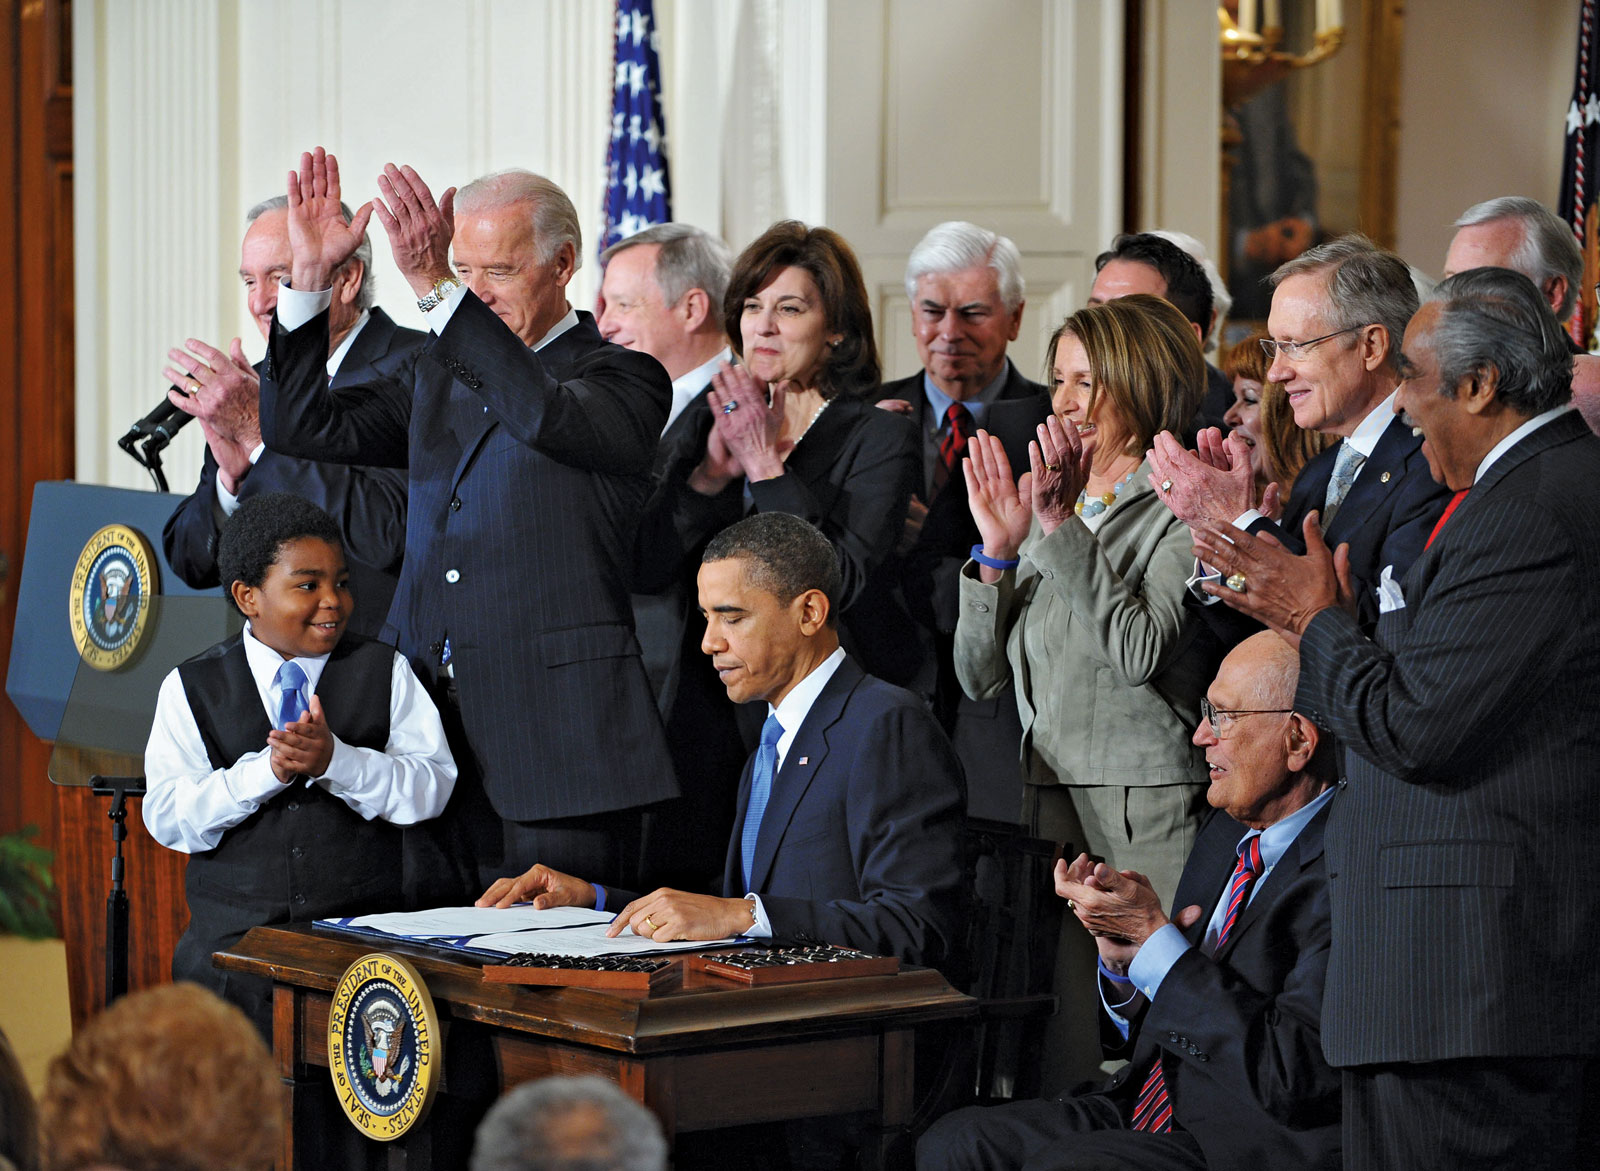
\includegraphics[scale=0.075]{ACA_signing.jpg}
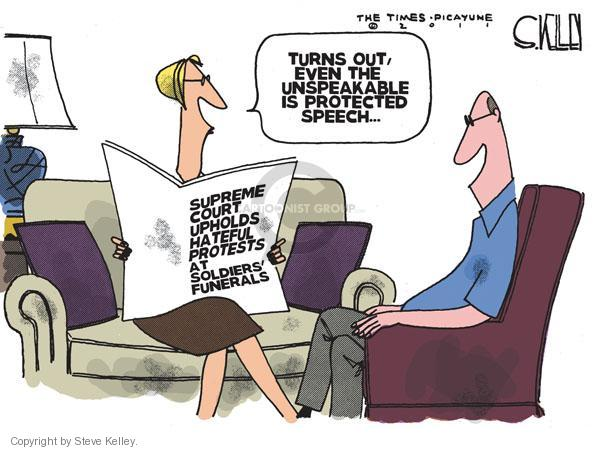
\includegraphics[scale=0.2]{WBC_synder.jpg}
\end{center}
\end{column}
\end{columns}
\end{frame}

%%@@@@@@@@@@@@@@@@@@@@@@@@@@@@@@@@@@@@@@@@@@@@@@@@@
%\begin{frame}
%\frametitle{Paradox examples:}
%\begin{columns}
%\begin{column}{0.5\textwidth}
%\begin{itemize}
%\item Industry support for regulation;
%\begin{itemize}
%\item Government regulation imposes costs and crushes innovation  $=$ voluntary standards;
%\item Regulation levels the playing field and limits liability;
%\item For or against?
%\end{itemize}
%\bigskip
%\item The Second Gulf War;
%\begin{itemize}
%\item Sadam Hussein allied to OBL?
%\item WMD?
%\item Democratization?
%\item Fixed flawed earlier policy?
%\item Energy?
%\item Problem $\Rightarrow$ solution or solution $\Rightarrow$ problem?
%\end{itemize}
%\end{itemize}
%\end{column}
%\begin{column}{0.5\textwidth}
%\begin{center}
%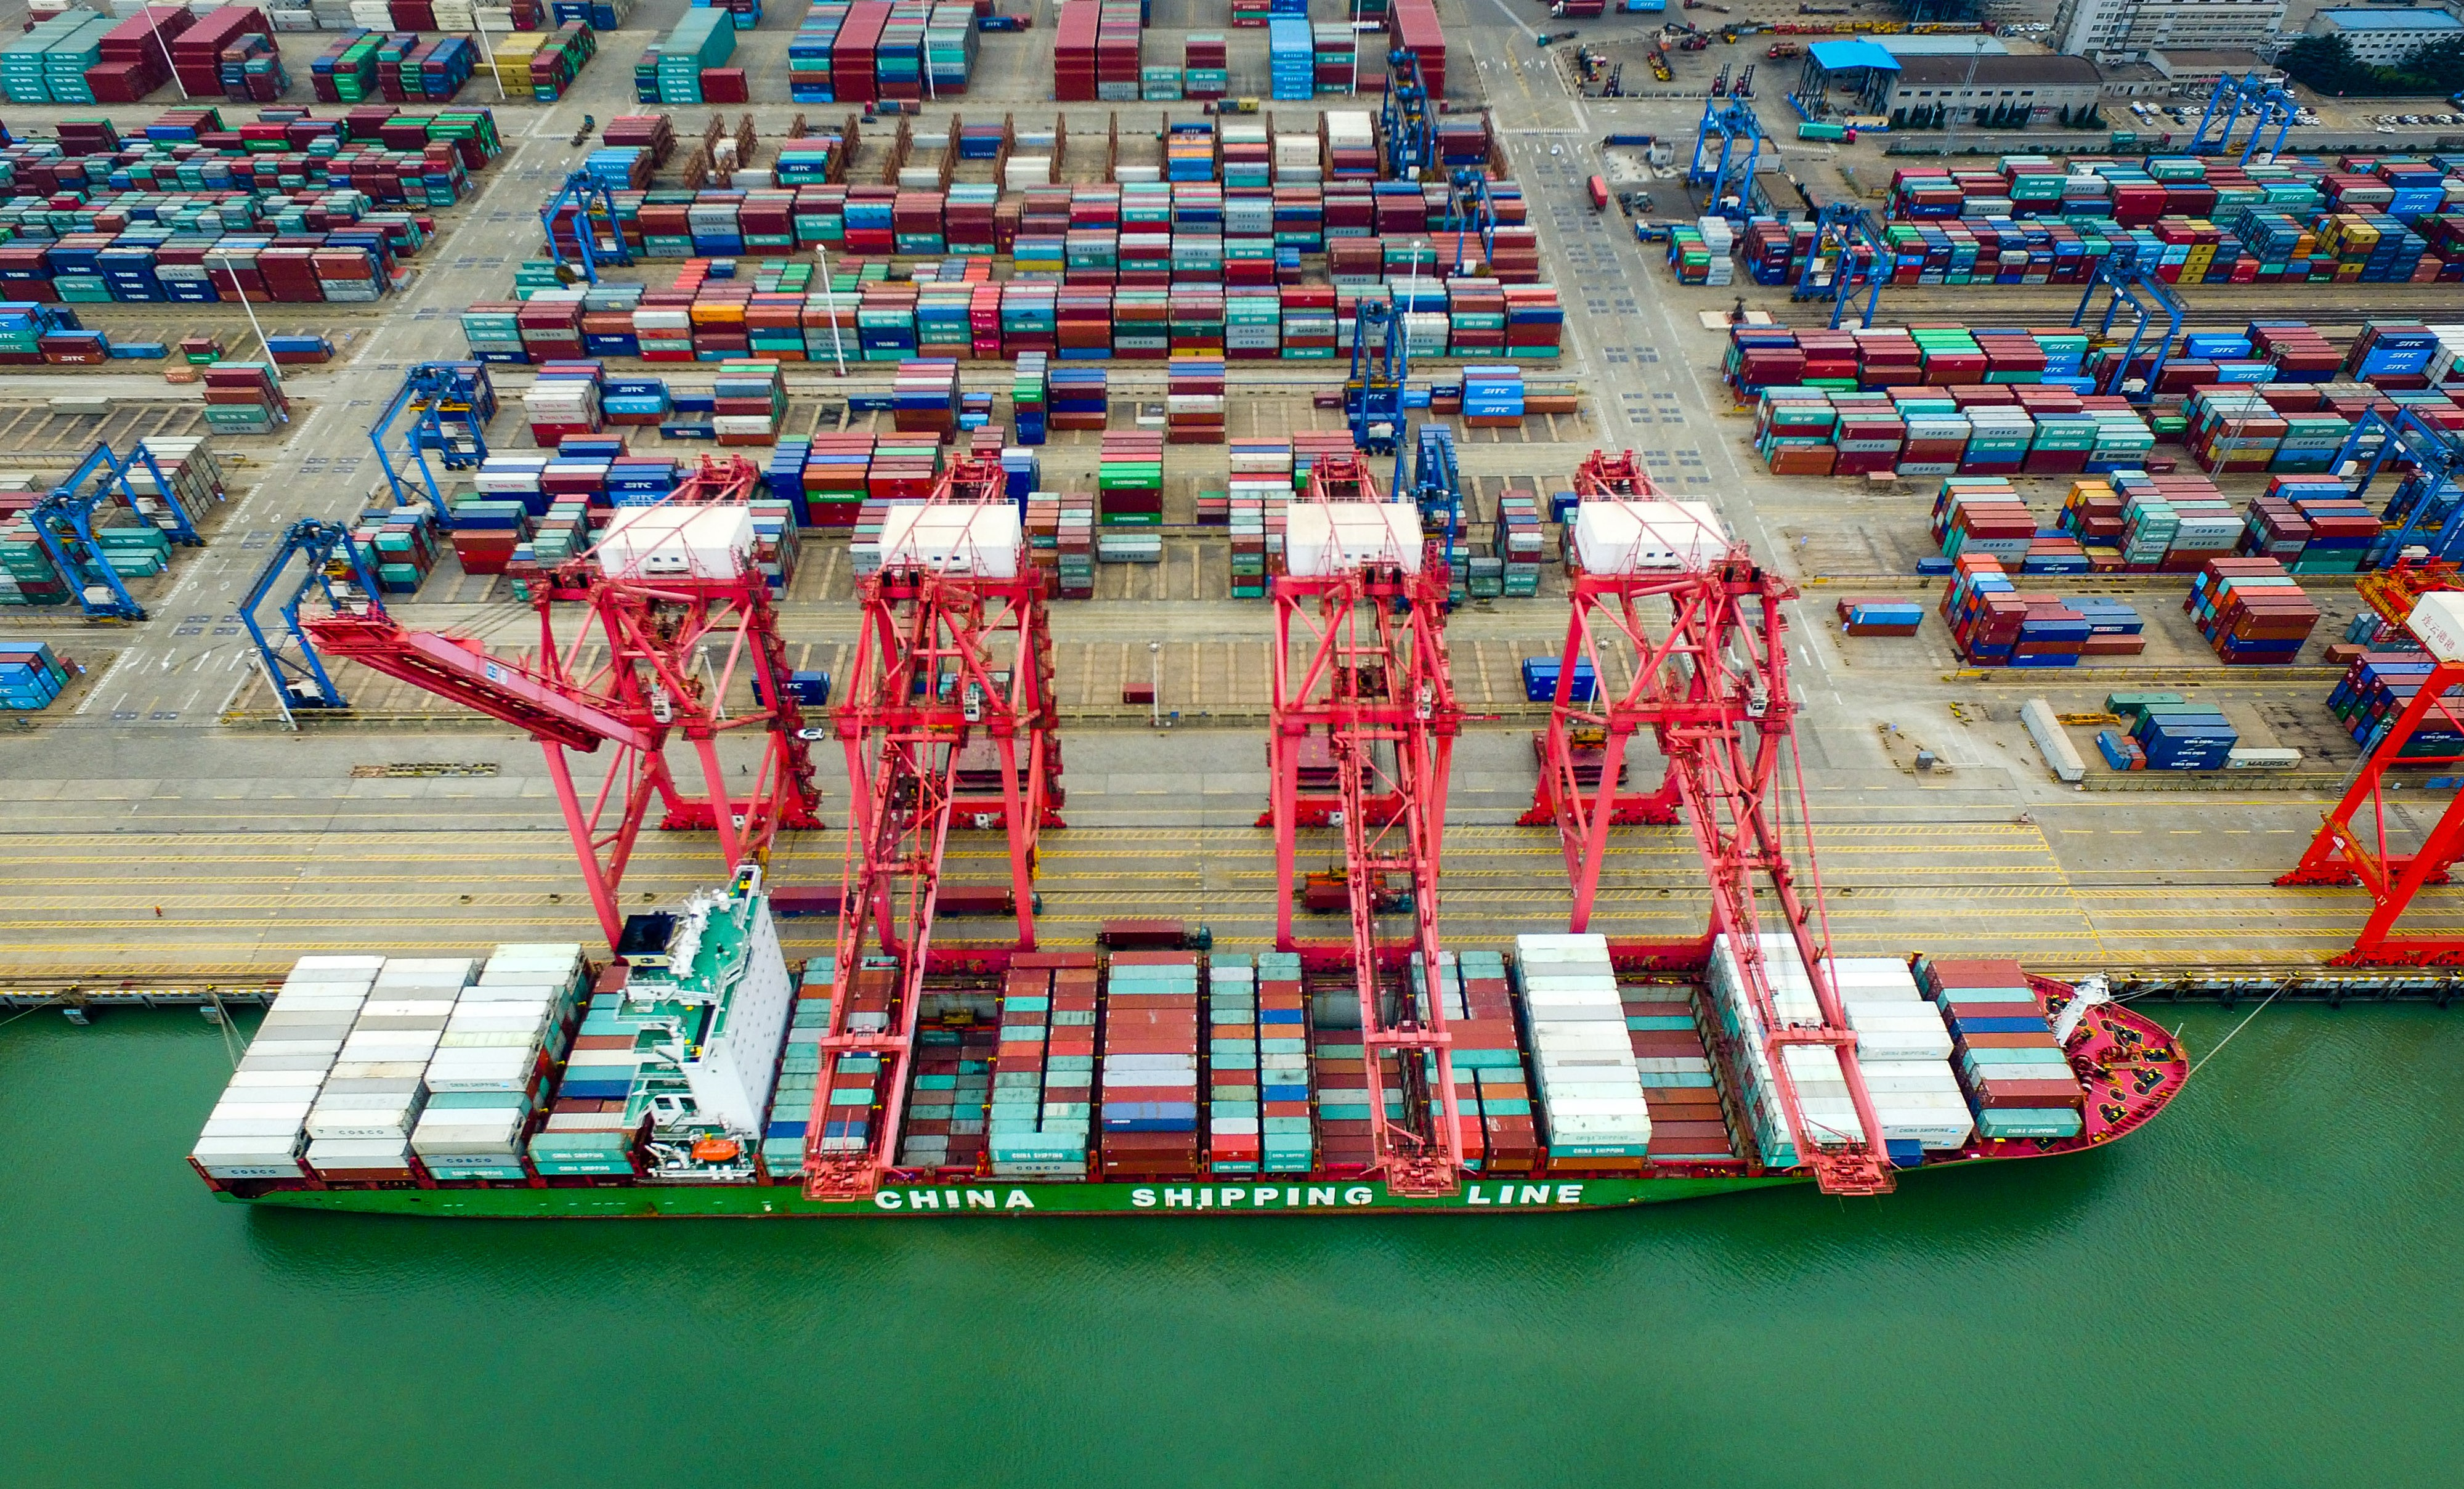
\includegraphics[scale=0.037]{cheap_imports.JPG}
%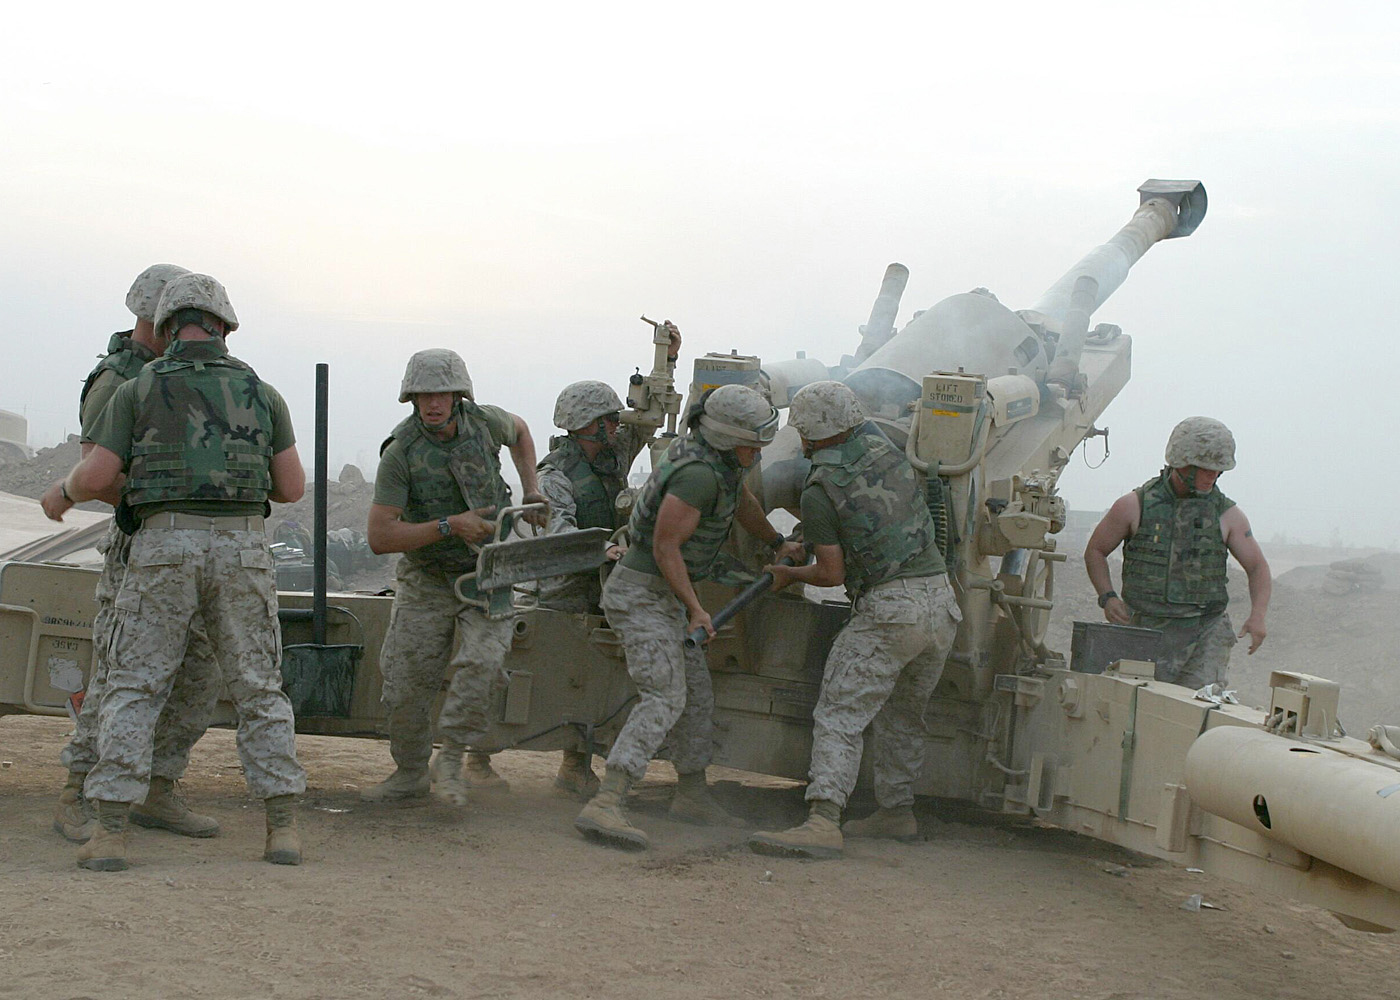
\includegraphics[scale=0.3]{artillery.jpg}
%\end{center}
%\end{column}
%\end{columns}
%\end{frame}
%
%%@@@@@@@@@@@@@@@@@@@@@@@@@@@@@@@@@@@@@@@@@@@@@@@@@
%\begin{frame}
%\frametitle{Paradox examples:}
%\begin{columns}
%\begin{column}{0.5\textwidth}
%\begin{itemize}
%\item Iranian raw materials imported into Iraq:
%\begin{itemize}
%\item ...enabled better quality of life amidst the conflict...
%\item ...crushed local economic development...
%\item Are low prices good or bad?
%\end{itemize}
%\bigskip
%\item Aftermath of Hurricane Katrina;
%\begin{itemize}
%\item Houses knocked down and shifted from foundations;
%\item City wanted to remove obstacles to traffic but owners wanted to protect property;
%\item Junk or treasure?
%\end{itemize}
%\end{itemize}
%\end{column}
%\begin{column}{0.5\textwidth}
%\begin{center}
%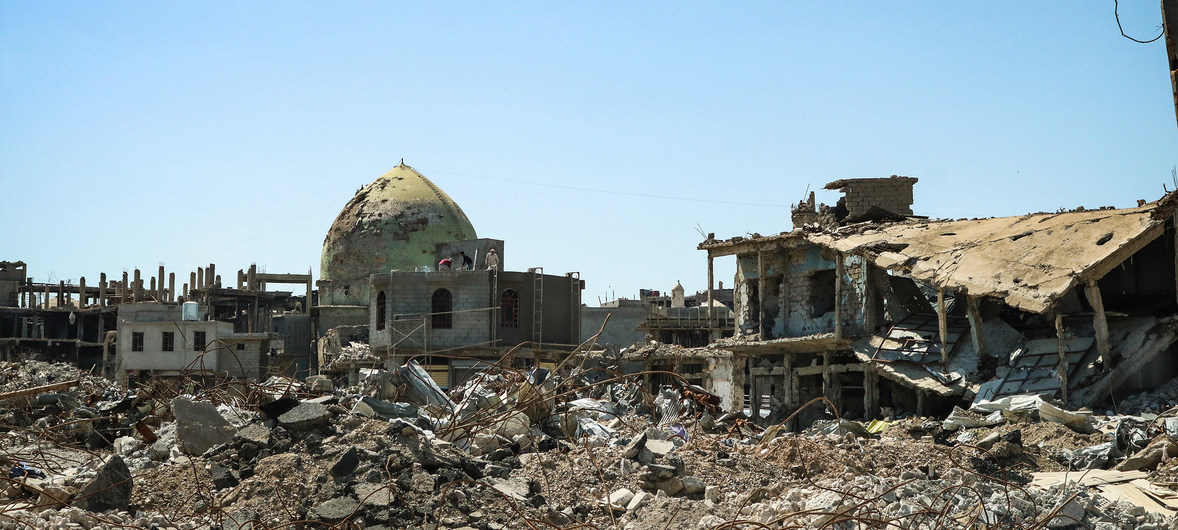
\includegraphics[scale=0.15]{iraqwar.jpg}
%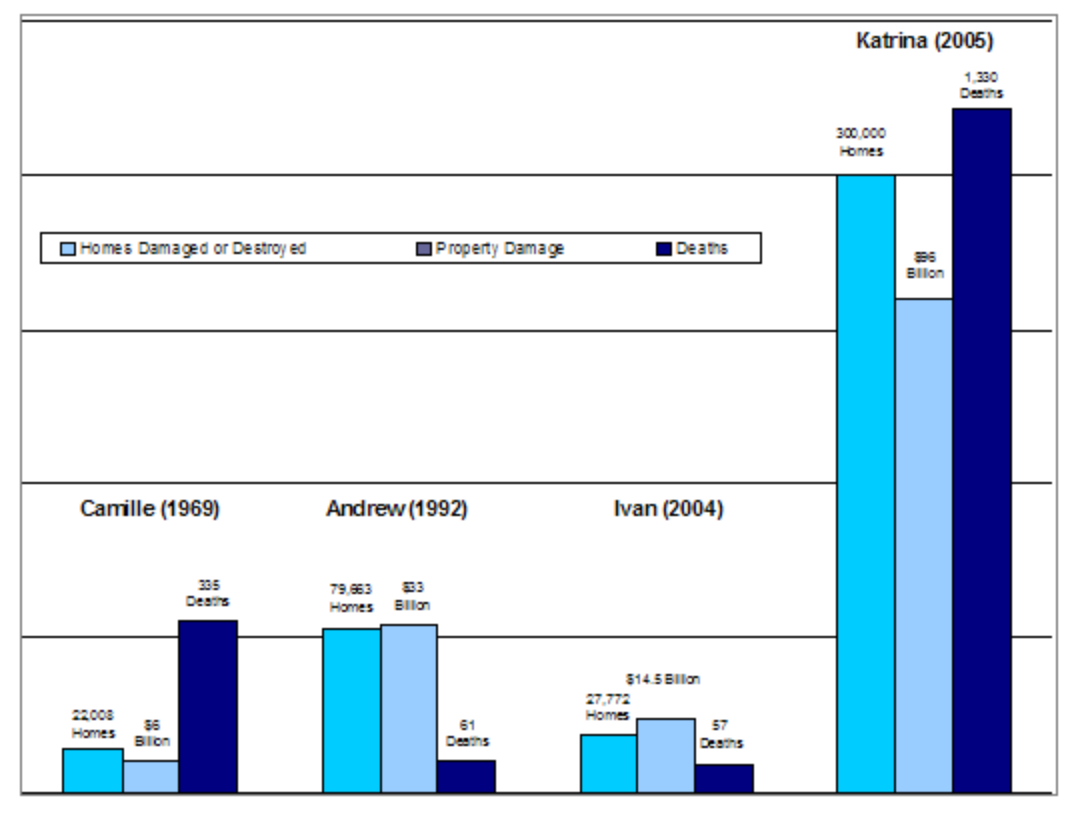
\includegraphics[scale=0.27]{katrina.png}
%\end{center}
%\end{column}
%\end{columns}
%\end{frame}
%
%%@@@@@@@@@@@@@@@@@@@@@@@@@@@@@@@@@@@@@@@@@@@@@@@@@
%\begin{frame}
%\frametitle{Paradox examples:}
%\begin{columns}
%\begin{column}{0.5\textwidth}
%\begin{itemize}
%\item Multiculturalism or universal rights:
%\begin{itemize}
%\item Chinese-American man bludgeoned wife to death;
%\item Convicted of manslaughter after cultural defense;
%\item Assimilation good or bad?
%\end{itemize}
%\bigskip
%\item Guantanamo:
%\begin{itemize}
%\item a convenience that offers an opportunity to hold dangerous individuals;
%\item an injustice that creates significant spur to terrorist recruiting;
%\item Are we more or less secure?
%\end{itemize}
%\end{itemize}
%\end{column}
%\begin{column}{0.5\textwidth}
%\begin{center}
%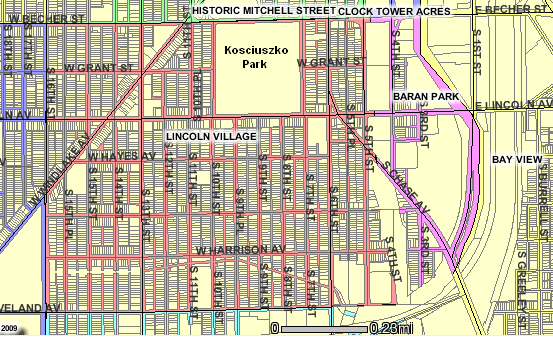
\includegraphics[scale=0.27]{LincolnVillageBlocks.png}
%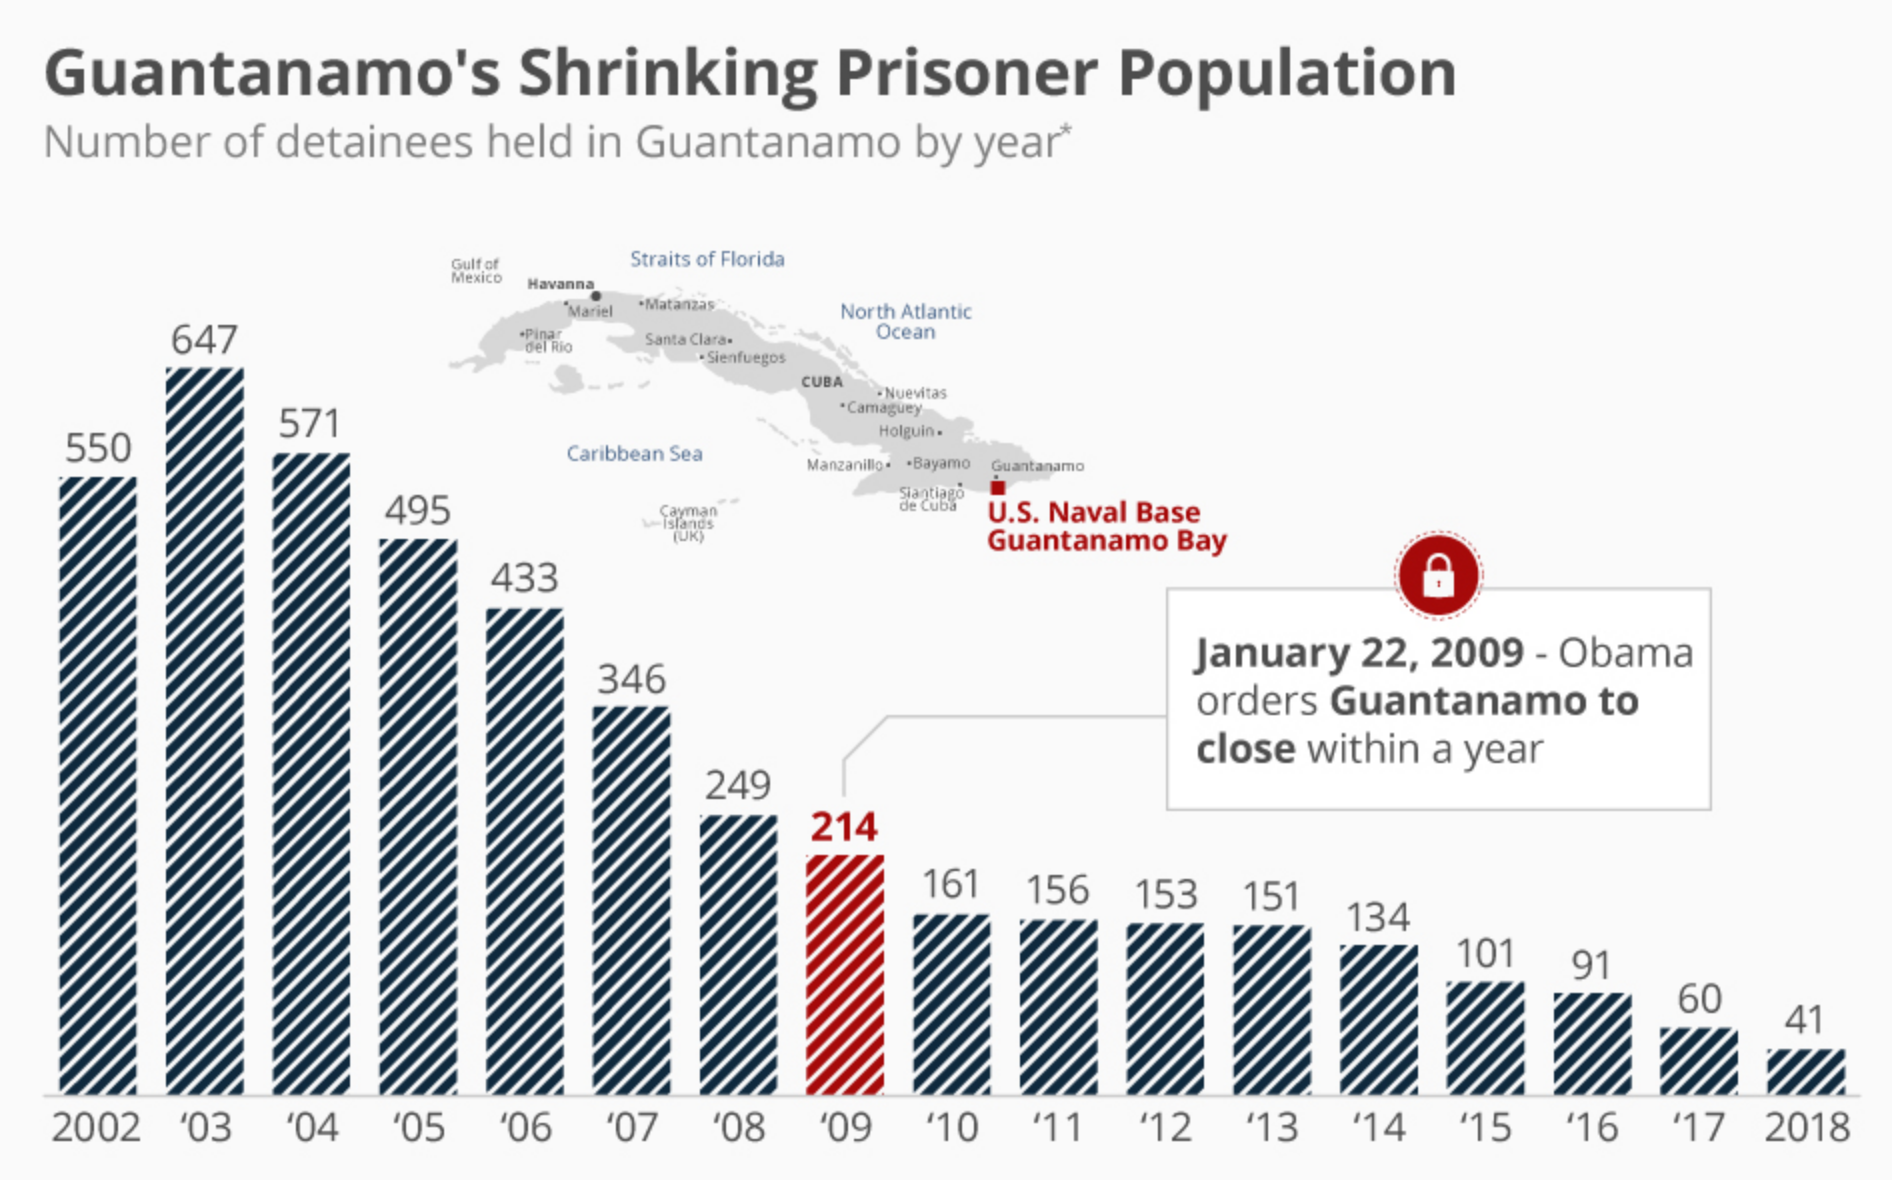
\includegraphics[scale=0.18]{guantanamo.png}
%\end{center}
%\end{column}
%\end{columns}
%\end{frame}

%@@@@@@@@@@@@@@@@@@@@@@@@@@@@@@@@@@@@@@@@@@@@@@@@@
\begin{frame}
\frametitle{How can we resolve these paradoxes?}

\begin{itemize}
\item The `rationality project' (sidelines politics);
\bigskip
\begin{itemize}
\item Goal: make policy via rational, analytic, scientific methods;
\bigskip
\item Examples:
\begin{itemize}
\item Constitutional design;
\item Inductive analysis applied to appellate court decisions;
\item Policy making authority taken from elected bodies and given to experts;
\item Undergrad/grad eduction in public policy;
\item Rational choice in academia;
\end{itemize}
\end{itemize}
\bigskip
\bigskip
\item The polis -- Stone's approach (embraces politics);
\bigskip
\bigskip
\item Read critically:
\begin{itemize}
\item Stone is setting the rationality project up to fail -- it is a strawman;
\item Critiques of the rationality project are positivist critiques (e.g. it is falsified by the data) but the rationality project itself might be best thought of as normative;
\end{itemize}

\end{itemize} 

\end{frame}

%@@@@@@@@@@@@@@@@@@@@@@@@@@@@@@@@@@@@@@@@@@@@@@@@@
\begin{frame}
\frametitle{The Rationality Project}

\begin{itemize}
\item \textbf{Model of reasoning}:
\begin{itemize}
\item identify objectives;
\item identify actions to achieve objectives;
\item Predict consequences of each alternative;
\item Evaluate the consequences of each alternative;
\item Optimize;
\item Criticism: fails to tell Obama what to do; ignores emotions; ignores ethics
\end{itemize}
\bigskip
\item \textbf{Model of society}:
\begin{itemize}
\item Market: society is a collection of autonomous, rational decision makers who come together only when they want to make an exchange;
\item fixed, independent preferences maximized via rational calculation;
\item Criticism: connections are varied, preferences are inconsistent;
\end{itemize}
\bigskip
\item \textbf{Model of policy making}:
\begin{itemize}
\item Stages model of policy making;
\item Birkland+ model of policy making;
\item ACF, etc.
\end{itemize}

\end{itemize} 

\end{frame}

%@@@@@@@@@@@@@@@@@@@@@@@@@@@@@@@@@@@@@@@@@@@@@@@@@
\begin{frame}
\begin{center}
\Large Polis: a model of a political society with simple forms of organizations large enough to allow for politics
\end{center}
\begin{itemize}
\item community(ies) with community-level ideas, images, will, and effort;
\item both self-interest and altruism are important for choices;
\item public interest;
\item problems are commons problems;
\item influence and coercion are important;
\item cooperation and competition are important;
\item loyalty is normal;
\item groups are main building blocks;
\item information is not objective.
\end{itemize}
\end{frame}

%@@@@@@@@@@@@@@@@@@@@@@@@@@@@@@@@@@@@@@@@@@@@@@@@@
\begin{frame}
\frametitle{Community}
\begin{itemize}
\item \textbf{Because politics and policy can happen only in communities they must be the starting point of our polis...}
\bigskip
\item Characteristics of a community:
\begin{itemize}
\item Members!
\item Decision criteria to determine who is in and who is out (e.g. citizenship) 
\item Procedures to determine who can join (e.g. US citizenship test);
\item Rules and authority (e.g. the constitution);
\item Social, economic, and political rights and benefits (e.g. use of the golf course);
\end{itemize}
\bigskip
\bigskip
\item \textbf{Cultural} community -- shared culture/identities derived from shared language, history, and traditions;
\bigskip
\bigskip
\item \textbf{Political} community -- group who live under the same political rules/governance;
\bigskip
\bigskip
\item Collective will.
\end{itemize}
\end{frame}

%@@@@@@@@@@@@@@@@@@@@@@@@@@@@@@@@@@@@@@@@@@@@@@@@@
\begin{frame}
\frametitle{Community}
\begin{center}
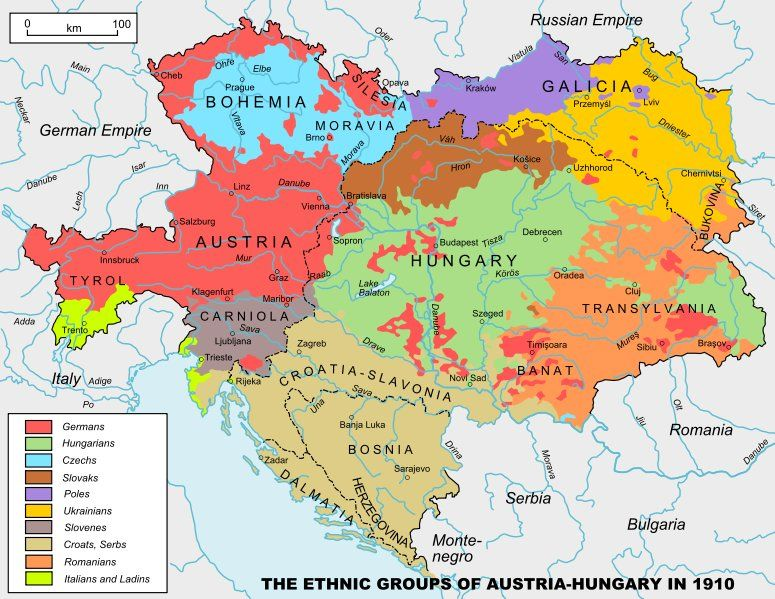
\includegraphics[scale=0.33]{mapempire.jpg}
\end{center}

\end{frame}

%@@@@@@@@@@@@@@@@@@@@@@@@@@@@@@@@@@@@@@@@@@@@@@@@@
\begin{frame}
\frametitle{Community}
When thinking about collective will remember:
\bigskip
\bigskip
\begin{center}
\large \textbf{Arrows Theorem: no ranked voting electoral system can convert individual ranked preferences into a community-wide ranking ‘rationally’ except dictatorship.}
\end{center}
\end{frame}

%@@@@@@@@@@@@@@@@@@@@@@@@@@@@@@@@@@@@@@@@@@@@@@@@@
\begin{frame}
\frametitle{Individual interest: self-interest}
\begin{center}
\Huge \textbf{Individual welfare.}
\end{center}
\end{frame}

%@@@@@@@@@@@@@@@@@@@@@@@@@@@@@@@@@@@@@@@@@@@@@@@@@
\begin{frame}
\frametitle{Individual interest: altruism}
\begin{itemize}
\item \textbf{Humans care about others so a model of political community must recognize altruism as a powerful human motive...}
\bigskip
\bigskip
\item But does altruism exist?
\begin{itemize}
\item `No man giveth but with intention of good to himself' $\sim$ Hobbes;
\item Data: altruistic action $=$ satisfaction, fulfillment, meaning;
\end{itemize}
\bigskip
\bigskip
\item Does it matter?
\begin{itemize}
\item can think of altruism as acting in order to benefit others rather than oneself...
\item OR as maximizing elements of personal happiness that also help others;
\item claim: they are observationally equivalent.
\end{itemize}
\end{itemize}
\end{frame}

%@@@@@@@@@@@@@@@@@@@@@@@@@@@@@@@@@@@@@@@@@@@@@@@@@
\begin{frame}
\frametitle{Public Interest}
\begin{itemize}
\item \textbf{Public interest}: the welfare of the general public; ex ante welfare of the representative individual; the social preference;
\bigskip
\item According to the rationality project, the public interest is discoverable;
\bigskip
\bigskip
\item According to Stone, the public interest is contested;
\bigskip
\bigskip
\item Some of the ways one might try to identify what is in the public interest:
\begin{itemize}
\item Aggregated individual private interests;
\item Aggregated individual interests for their community–``public-spirited self-interest";
\item Goals on which there is consensus or a majority;
\item Things that are good for a community as a community (order, rules, stability, defense).
\end{itemize}
\end{itemize}
\end{frame}

%@@@@@@@@@@@@@@@@@@@@@@@@@@@@@@@@@@@@@@@@@@@@@@@@@
\begin{frame}
\frametitle{What sorts of problems are we going to deal with?}
\begin{center}
\Large \textbf{Commons problems}: where private gains mean public costs (e.g. pollution) OR where public gains mean private costs (e.g. taxes).
\end{center}
\end{frame}

%@@@@@@@@@@@@@@@@@@@@@@@@@@@@@@@@@@@@@@@@@@@@@@@@@
\begin{frame}
\frametitle{Bridging individual interest and public interest}
\begin{itemize}
\item \textbf{Influence};
\begin{itemize}
\item Getting an actor to do something they would not otherwise do;
\item Influence = coercion?  
\end{itemize}
\bigskip
\bigskip
\item \textbf{Cooperation}:
\begin{itemize}
\item Politics = building alliances to compete with opponents (are two person interactions `politically empty'?);
\item An essential expression of power;
\item Good or bad?  Depends on context -- in economic activity described as collusion, price-fixing, etc., -- in politics described as coalition, support, etc.;
\end{itemize}
\bigskip
\bigskip
\item \textbf{Loyalty};
\begin{itemize}
\item `Sticky' or `stretchy' relationships.
\end{itemize}
\end{itemize}
\end{frame}

%@@@@@@@@@@@@@@@@@@@@@@@@@@@@@@@@@@@@@@@@@@@@@@@@@
\begin{frame}
\frametitle{Groups}
\begin{itemize}
\item Influence/cooperation/loyalty lead to \textbf{group formation} which are the `building blocks' of the polis;
\bigskip
\bigskip
\item Groups are important for three reasons:
\begin{itemize}
\item Individuals depend on \textbf{groups to represent interests} (e.g. unions);
\item Policy making in part explained by how \textbf{groups form/split dynamically} to achieve public purpose;
\item Decisions of the polis are expressed in terms of \textbf{preferences aggregated at group level} (e.g. via voting);
\end{itemize}
\bigskip
\bigskip
\item Is this self-contradictory?  Groups are Stone's building blocks but according to Stone they don't act with a single mind...
\end{itemize}
\end{frame}

%@@@@@@@@@@@@@@@@@@@@@@@@@@@@@@@@@@@@@@@@@@@@@@@@@
\begin{frame}
\frametitle{Information}
\begin{itemize}
\item According to Stone \textbf{market information} $=$ accurate, complete, and costless (it needn't be);
\bigskip
\bigskip
\item \textbf{Polis information} $=$ ambiguous, incomplete, possibly purposefully withheld;
\begin{itemize}
\item Policy is complicated -- hard to find the right causal models;
\item Education is required to acquire knowledge and is not uniformly distributed;
\end{itemize}
\bigskip
\bigskip
\item Implications:
\begin{itemize}
\item $\Rightarrow$ interpretations are more important than `facts';
\item $\Rightarrow$ information revelation is strategic;
\item $\Rightarrow$ actors will fight to control interpretations.
\end{itemize}
\end{itemize}
\end{frame}

%%@@@@@@@@@@@@@@@@@@@@@@@@@@@@@@@@@@@@@@@@@@@@@@@@@
%\begin{frame}
%\frametitle{Power}
%\begin{itemize}
%\item Getting an actor to do something they would not otherwise do -- subordinate individual self-interest to:
%\begin{itemize}
%\item Other individuals' interests;
%\item Group interests;
%\item Public interest;
%\end{itemize} 
%\bigskip
%\bigskip
%\item Operates through influence, cooperation, loyalty, strategic information control, expressed in ideas and portrayals of ideas about policy;
%\bigskip
%\bigskip
%\item Can be counted as a resource (e.g. money, votes, titles).
%\end{itemize}
%\end{frame}
%
%%@@@@@@@@@@@@@@@@@@@@@@@@@@@@@@@@@@@@@@@@@@@@@@@@@
%\begin{frame}
%\begin{center}
%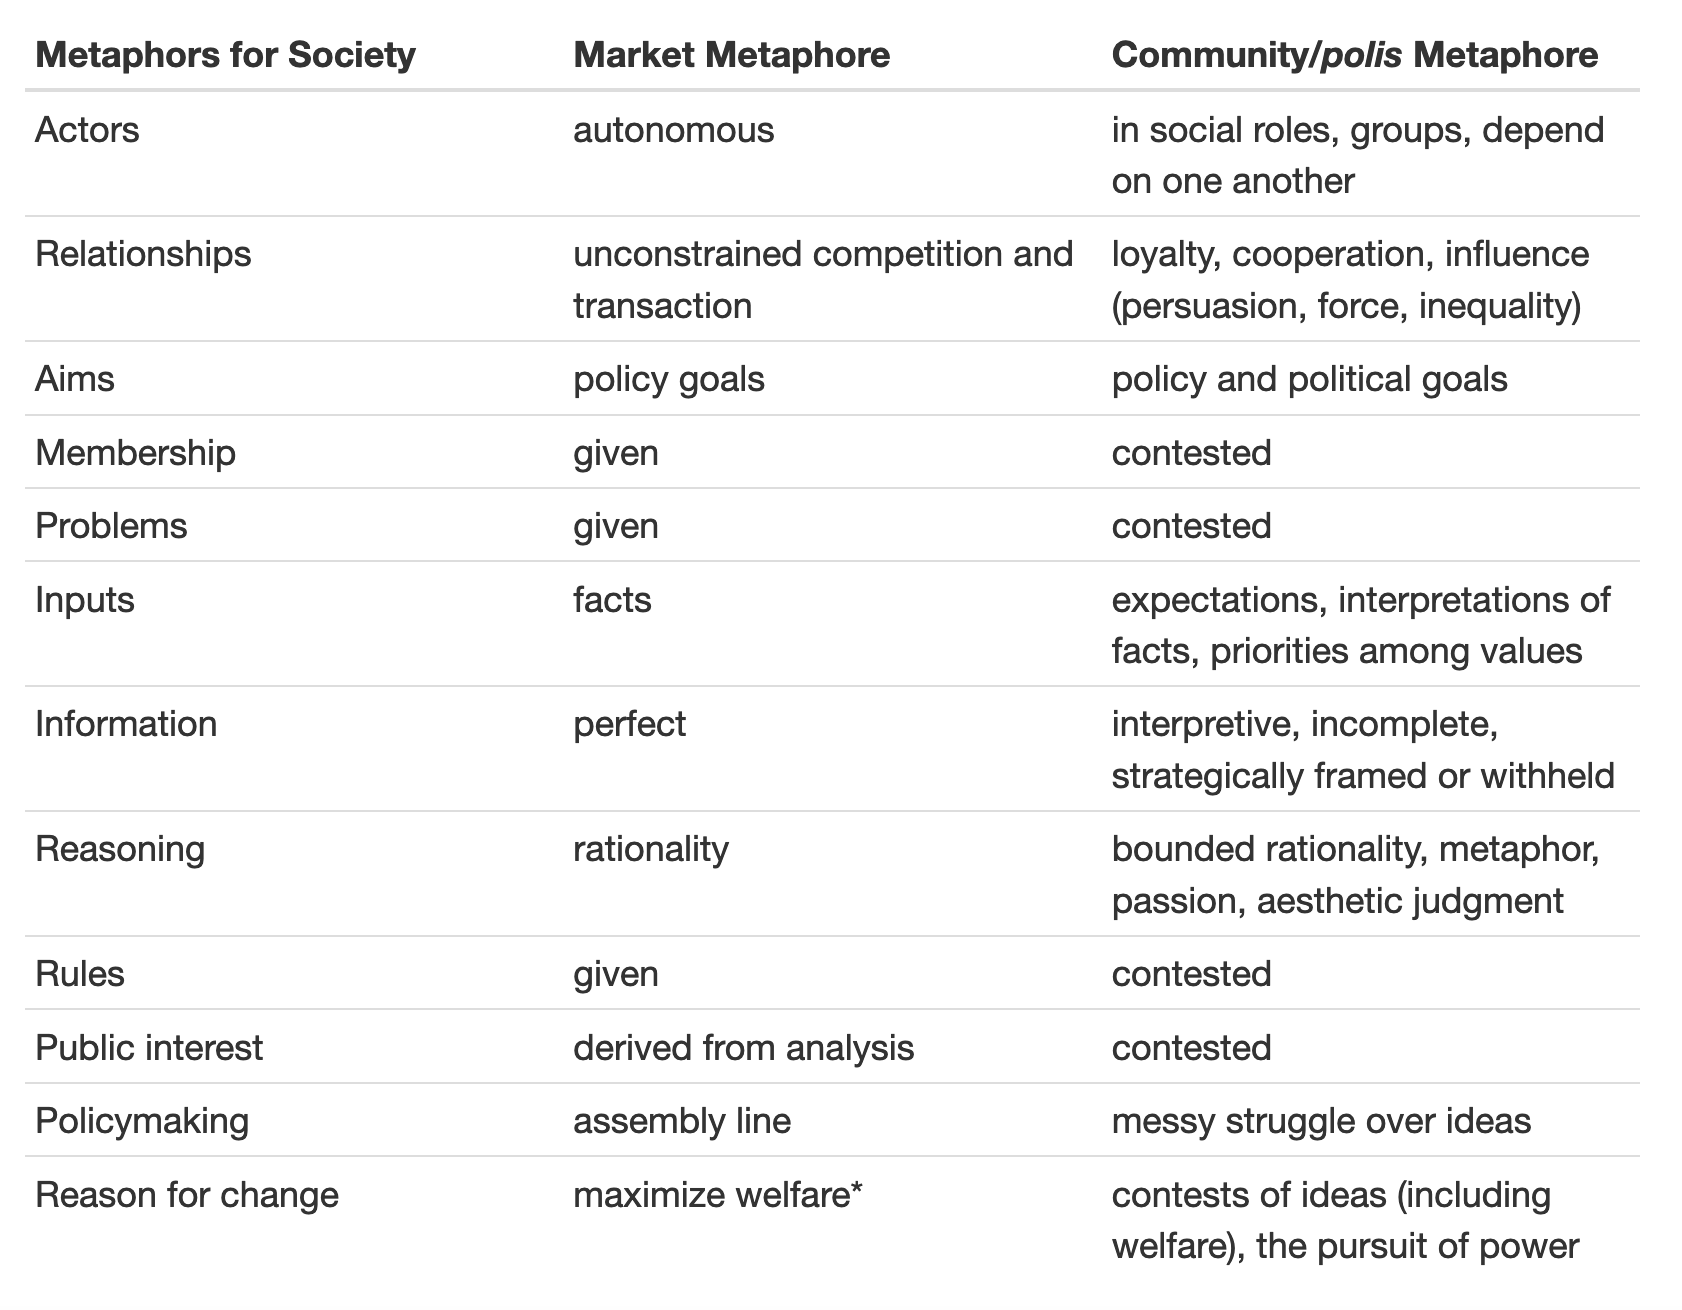
\includegraphics[scale=0.33]{summary.png}
%\end{center}
%\end{frame}

%%@@@@@@@@@@@@@@@@@@@@@@@@@@@@@@@@@@@@@@@@@@@@@@@@@
%\begin{frame}
%\frametitle{Food for thought...}
%
%\begin{itemize}
%\item Is society better imagined as a market or Stone's polis?
%\bigskip
%\bigskip
%\item How we see society affects the things we think about when making policy.
%\begin{itemize}
%\item  If society $=$ polis how does that lead us to think about who belongs?
%\item If society $=$ market how does this lead us to think about who belongs?
%\end{itemize}
%\bigskip
%\bigskip
%\item Which metaphor puts more emphasis on questions of membership?
%\end{itemize}
%
%\end{frame}

%@@@@@@@@@@@@@@@@@@@@@@@@@@@@@@@@@@@@@@@@@@@@@@@@@
\begin{frame}
%\frametitle{Foreign Policy Making}

\begin{center}
\Huge\textbf{Goals}
\end{center}

\end{frame}

%@@@@@@@@@@@@@@@@@@@@@@@@@@@@@@@@@@@@@@@@@@@@@@@@@
\begin{frame}
%\frametitle{Foreign Policy Making}

\begin{center}
\huge\textbf{Whose goals?!}
\end{center}

\end{frame}

%@@@@@@@@@@@@@@@@@@@@@@@@@@@@@@@@@@@@@@@@@@@@@@@@@
\begin{frame}

Federalist Papers No. 68: The Mode of Electing the President (Hamilton)
\begin{itemize} 
\item \small ``It was desirable that the sense of the people should operate in the choice of the person to whom so important a trust was to be confided."
\bigskip
\item ``It was equally desirable that the immediate election should made by men most capable of analyzing the qualities adapted to the station and acting under circumstances favorable to deliberation, and to a judicious combination of all the reasons and inducements which were proper to govern their choice."
\bigskip
\item ``It was also particularly desirable to afford as little opportunity as possible to tumult and disorder."
\bigskip
\item ``Nothing was more to be desired than that every practicable obstacle should be opposed to cabal, intrigue, and corruption."
\bigskip
\item ``Another and no less important desideratum was that the executive should be independent for his continuance in office on all but the people themselves."
\end{itemize}

\end{frame}

%@@@@@@@@@@@@@@@@@@@@@@@@@@@@@@@@@@@@@@@@@@@@@@@@@
\begin{frame}
%\frametitle{Foreign Policy Making}

\begin{center}
\huge\textbf{...to shape and sustain a peaceful, prosperous, just, and democratic world and foster conditions for stability and progress for the benefit of the American people and people everywhere.}
\end{center}

\end{frame}

%@@@@@@@@@@@@@@@@@@@@@@@@@@@@@@@@@@@@@@@@@@@@@@@@@
\begin{frame}
%\frametitle{Foreign Policy Making}

\begin{center}
\huge\textbf{...preempt threats and further US national security objectives by collecting intelligence that matters, producing objective all-source analysis, conducting effective covert action as directed by the President, and safeguarding the secrets that help keep our Nation safe.}
\end{center}

\end{frame}

%@@@@@@@@@@@@@@@@@@@@@@@@@@@@@@@@@@@@@@@@@@@@@@@@@
\begin{frame}
%\frametitle{Foreign Policy Making}

\begin{center}
\huge\textbf{...To protect and enhance our natural resources: our air, land and water; our wildlife, fish and forests and the ecosystems that sustain all life. To provide a healthy, sustainable environment and a full range of outdoor opportunities.}
\end{center}

\end{frame}

%@@@@@@@@@@@@@@@@@@@@@@@@@@@@@@@@@@@@@@@@@@@@@@@@@
\begin{frame}
%\frametitle{Foreign Policy Making}

\begin{center}
\huge\textbf{What are goals?}
\end{center}

\end{frame}

%@@@@@@@@@@@@@@@@@@@@@@@@@@@@@@@@@@@@@@@@@@@@@@@@@
\begin{frame}
%\frametitle{Foreign Policy Making}

\begin{itemize}
\item Goals dimensionalized:
\begin{itemize}
\item Equity;
\item Efficiency;
\item Welfare;
\item Liberty;
\item Security;
\bigskip
\end{itemize}
\item Goal have the feel of preferences over outcomes;
\bigskip
\item Two situations in which goals can lead to intractable conflict:
\begin{itemize}
\item 1) Pareto Optimality: a choice is Pareto optimal in a group setting when nobody can be made better off through a policy change without others being made worse off -- conflict when trying to change a Pareto optimal policy;
\item 2) Imagine two people one with weights given by $w$ and the other with weights given by $v$:
\begin{align*}
w_{1}*\mbox{Equity} + w_2*\mbox{Efficiency} + w_3*\mbox{Welfare} + w_4*\mbox{Liberty} + w_5*\mbox{Security}\\
v_{1}*\mbox{Equity} + v_2*\mbox{Efficiency} + v_3*\mbox{Welfare} + v_4*\mbox{Liberty} + v_5*\mbox{Security}
\end{align*}
Conflict when $w\neq v$.
\end{itemize}

\end{itemize}

\end{frame}

%@@@@@@@@@@@@@@@@@@@@@@@@@@@@@@@@@@@@@@@@@@@@@@@@@
\begin{frame}

\begin{center}
\Huge\textbf{Goals : Equity}\\
\bigskip
\bigskip
\bigskip
\normalsize Everybody wants it but people disagree over definitions
\end{center}

\end{frame}

%@@@@@@@@@@@@@@@@@@@@@@@@@@@@@@@@@@@@@@@@@@@@@@@@@
\begin{frame}
\frametitle{Definitions}
\begin{columns}
\begin{column}{0.5\textwidth}

\begin{itemize}
\item Politics is the authoritative distribution of resources;
\bigskip
\bigskip
\item All distributions have three parts:
\begin{itemize}
\item Who gets something;
\item What they get;
\item How the distribution is determined;
\end{itemize}
\bigskip
\bigskip
\item Equality denotes sameness in some part of the distribution of resources.
\end{itemize}
\end{column}

\begin{column}{0.5\textwidth}
\begin{center}
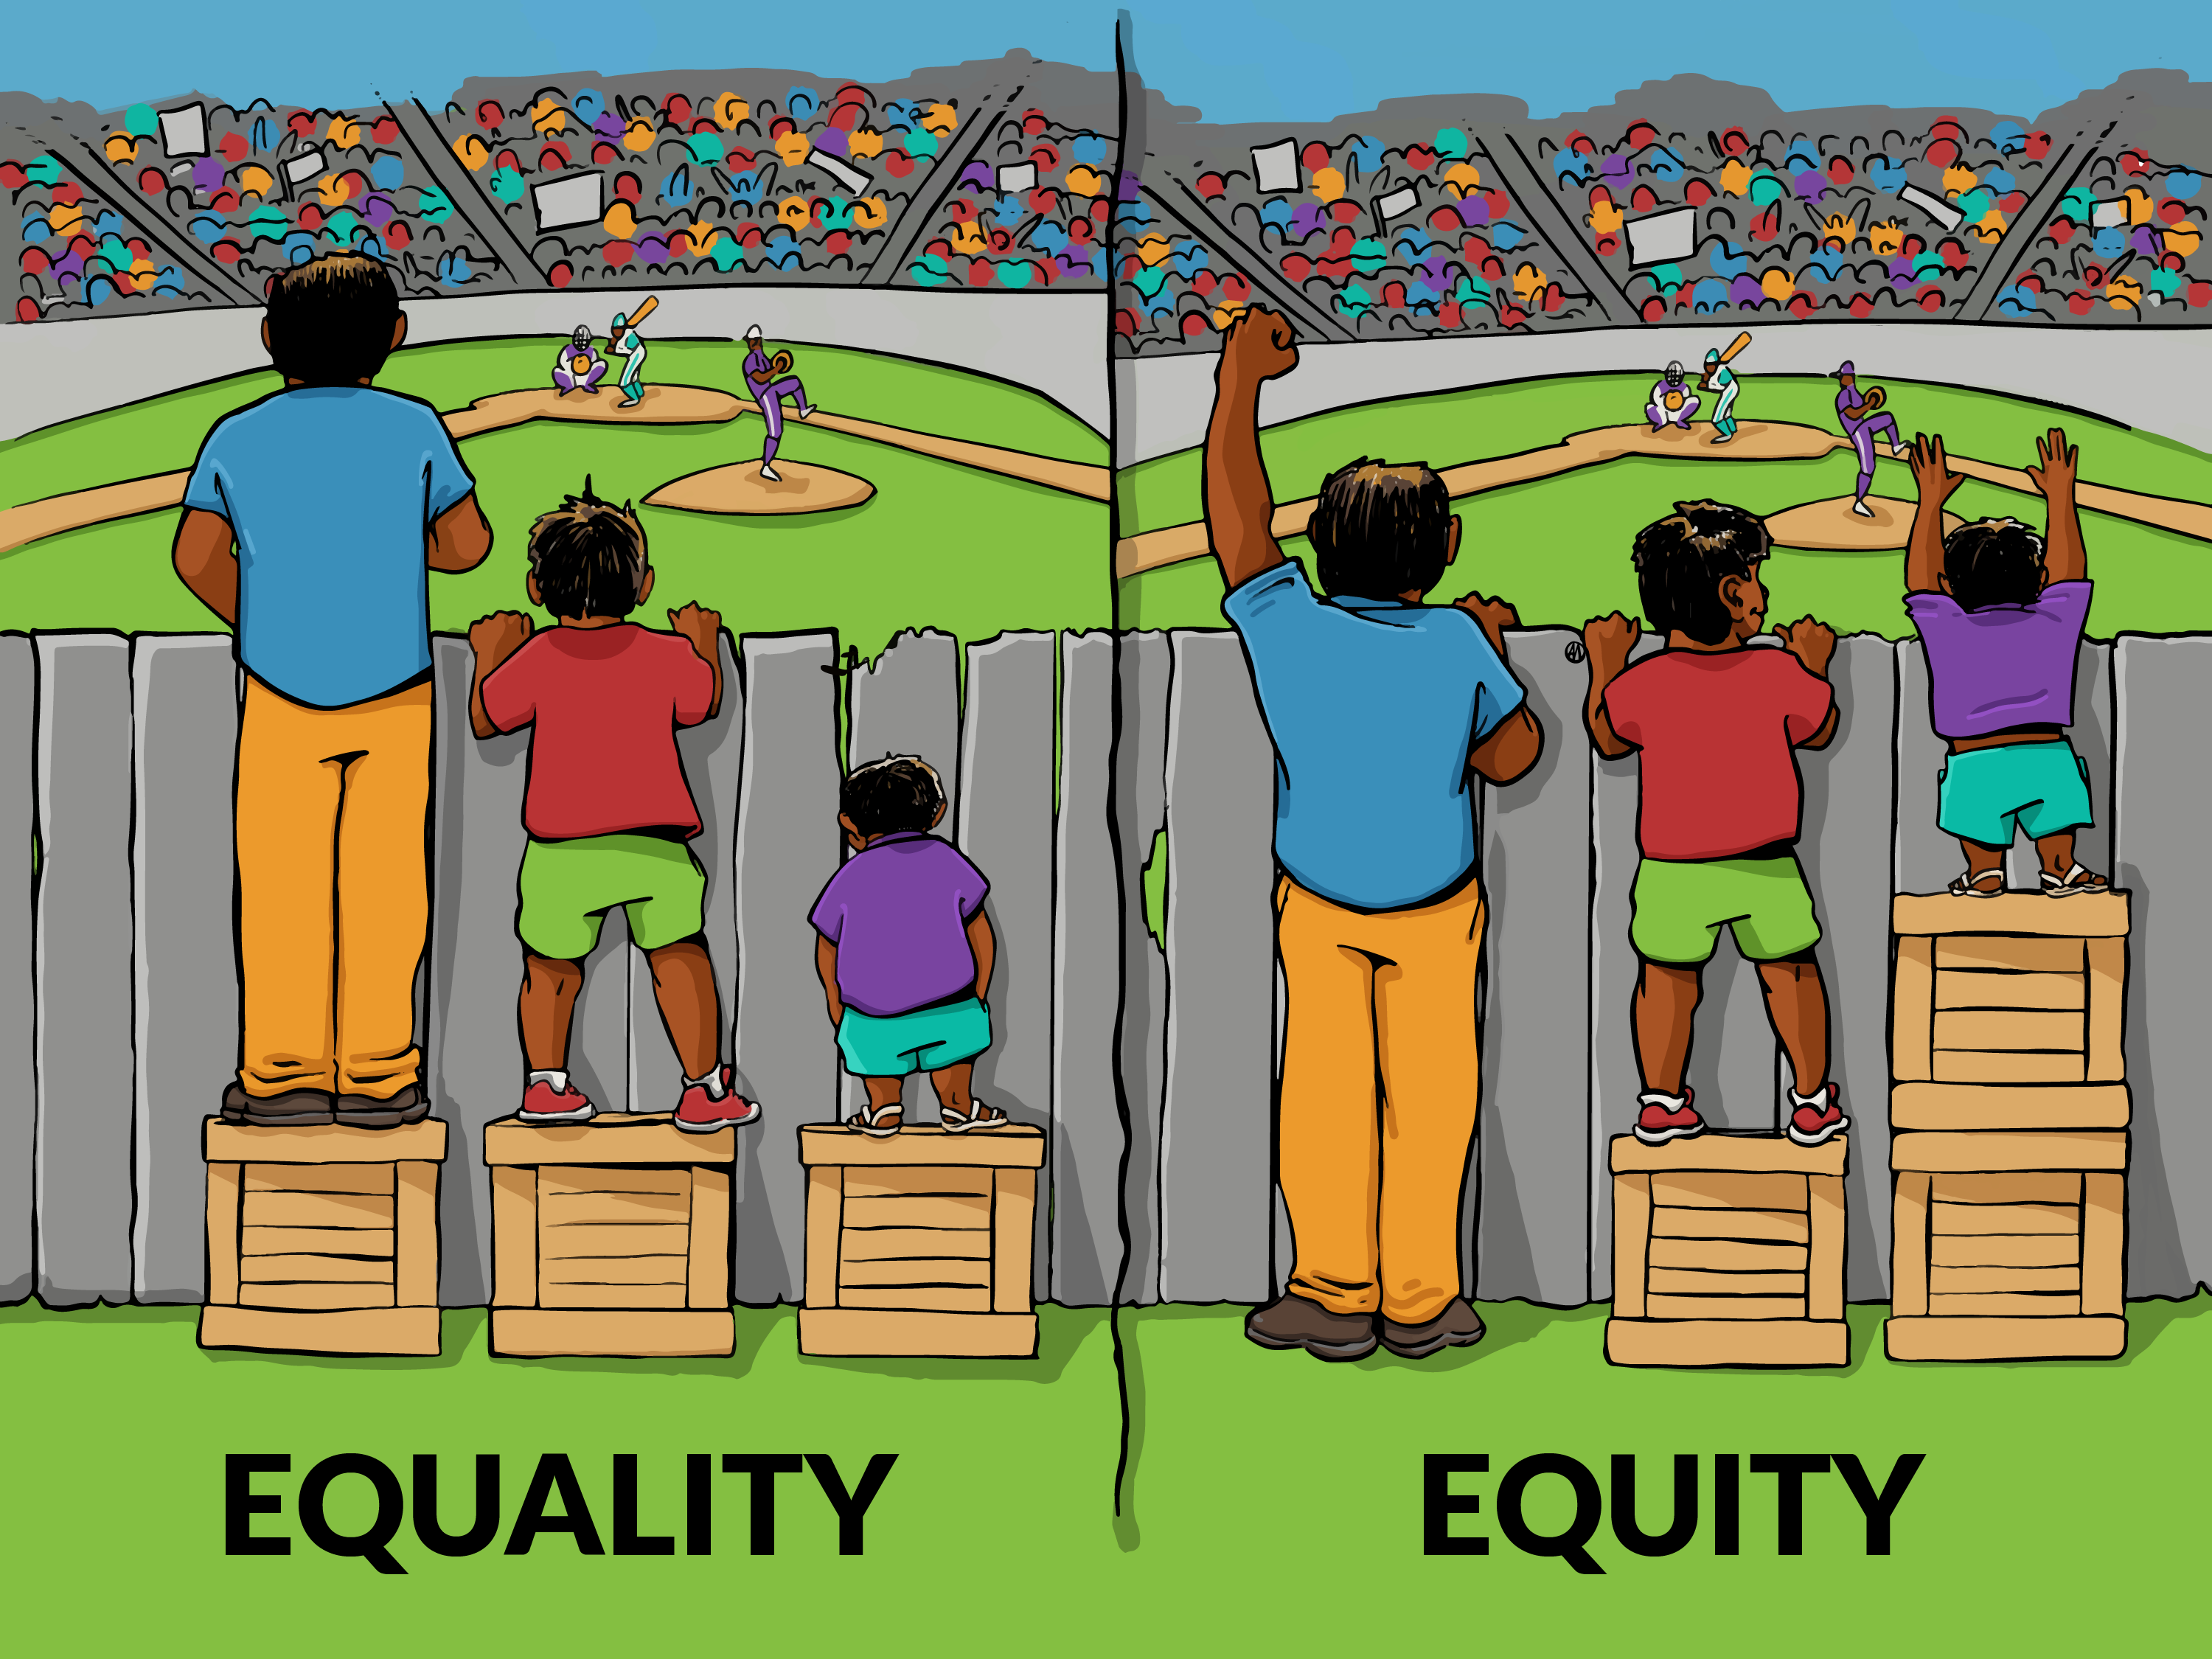
\includegraphics[scale=0.25]{EqualityEquity.png}
\end{center}
\end{column}
\end{columns}
\end{frame}

%EqualityEquity.png

%@@@@@@@@@@@@@@@@@@@@@@@@@@@@@@@@@@@@@@@@@@@@@@@@@
\begin{frame}
\frametitle{Dimensions: Membership}

\begin{itemize}
\item All members of a group get equal parts of something -- non-members get nothing;
\bigskip
\bigskip
\item Who is a member?!  This becomes a conflict over equity;
\bigskip
\bigskip
\item Some examples:
\begin{itemize}
\item 3/5s compromise;
\item Cherokee Nation membership;
\item EU citizens particular state membership;
\item Felony voting rights in the US;
\item Medicaid for immigrants;
\end{itemize}
\bigskip
\bigskip
\item Paradox: Equal slices, unequal invitations.
\end{itemize}

\end{frame}

%@@@@@@@@@@@@@@@@@@@@@@@@@@@@@@@@@@@@@@@@@@@@@@@@@
\begin{frame}
\frametitle{Dimensions: Merit}

\begin{itemize}
\item Maximize reward for individual achievement and minimize the role of immutable personal characteristics;
\bigskip
\bigskip
\item Measure and quantify `achievement' is hard.  How to measure becomes a conflict over equity;
\begin{itemize}
\item Admission tests (might be biased);
\item Increase in revenue (really needs counterfactual);
\end{itemize}
\bigskip
\bigskip
\item Is `effort' necessary or sufficient? How much $=$ luck/shoulders of giants?  
\begin{itemize}
\item If necessary but not sufficient, should `achievement' be rewarded at all?
\item If sufficient then a major justification for income inequality, but how much?
\end{itemize}
\bigskip
\bigskip
\item Paradox: (un)equal slices for (un)equal merit.
\end{itemize}

\end{frame}

%@@@@@@@@@@@@@@@@@@@@@@@@@@@@@@@@@@@@@@@@@@@@@@@@@
\begin{frame}
\frametitle{Dimensions: Rank}

\begin{itemize}
\item Society is a collection of subgroups and individual distribution should depend on membership in these subgroups;
\begin{itemize}
\item Government general schedule;
\item University community;
\end{itemize}
\bigskip
\bigskip
\item Rank membership/slices across ranks are conflicts over equity;
\bigskip
\bigskip
\item Does rank really measure some sort of quality we'd like to reward?
\bigskip
\bigskip
\item Paradox: (un)equal slices for (un)equal ranks.
\end{itemize}

\end{frame}

%@@@@@@@@@@@@@@@@@@@@@@@@@@@@@@@@@@@@@@@@@@@@@@@@@
\begin{frame}
\frametitle{Dimensions: Group-Based Distribution}

\begin{itemize}
\item Society is a collection of subgroups \textbf{defined by immutable personal characteristics} and individual distribution should depend on membership in these subgroups;
\bigskip
\bigskip
\item Often used to remedy history of unequal burden:
\begin{itemize}
\item VA benefits;
\item Affirmative actions;
\item Reparations for slavery;
\end{itemize}
\bigskip
\bigskip
\item Some challenges:
\begin{itemize}
\item Do the subgroups depict some useful social reality (e.g. are race and ethnicity `real')?
\item Identity characteristics may be only weakly correlated with historical burden;
\item Use of immutable characteristics are always illegitimate;
\end{itemize}
\bigskip
\bigskip
\item Paradox: unequal slices but equal social blocs.
\end{itemize}

\end{frame}

%@@@@@@@@@@@@@@@@@@@@@@@@@@@@@@@@@@@@@@@@@@@@@@@@@
\begin{frame}
\frametitle{Dimensions: Need}

\begin{itemize}
\item Use a particular distribution to compensate for shortfalls in the larger pattern of distribution;
\bigskip
\bigskip
\item What should the `larger pattern of distribution' include?
\begin{itemize}
\item Financial aid as a fraction of total assets (current earnings, future earning, family earnings);
\item Tax policy (income, wealth);
\end{itemize} 
\bigskip
\bigskip
\item Paradox: unequal slices but equal consumption.
\end{itemize}

\end{frame}

%@@@@@@@@@@@@@@@@@@@@@@@@@@@@@@@@@@@@@@@@@@@@@@@@@
\begin{frame}
\frametitle{Dimensions: Value}

\begin{itemize}
\item Switch from a standardized value to a customized value;
\bigskip
\bigskip
\item Some examples:
\begin{itemize}
\item Household specific poverty levels;
\item Job offers;
\item Auctions;
\end{itemize}
\bigskip
\bigskip
\item How do we estimate `value' - there are obvious incentives to misrepresent here;
\bigskip
\bigskip
\item Paradox: unequal slices but equal value.
\end{itemize}

\end{frame}

%@@@@@@@@@@@@@@@@@@@@@@@@@@@@@@@@@@@@@@@@@@@@@@@@@
\begin{frame}
\frametitle{Dimensions: Competition, Lotteries, Elections}

\begin{itemize}
\item Competition (e.g. markets):
\begin{itemize}
\item Allow relative merit to determine outcomes organically;
\item Paradox: unequal slices but fair competition w/ equal resources;
\end{itemize}
\bigskip
\bigskip
\item Lotteries (e.g. draft):
\begin{itemize}
\item Allow chance to determine outcomes stochastically;
\item Paradox: unequal slices but equal statistical chances;
\end{itemize}
\bigskip
\bigskip
\item Elections (e.g. for President):
\begin{itemize}
\item Aggregate preferences about how to distribute power;
\item Paradox: unequal slices but equal votes.
\end{itemize}
\end{itemize}

\end{frame}

%@@@@@@@@@@@@@@@@@@@@@@@@@@@@@@@@@@@@@@@@@@@@@@@@@
\begin{frame}
\frametitle{How to choose?!}

\begin{itemize}
\item Each of these dimensions yields different distributional outcomes:
\begin{itemize}
\item Membership, merit, rank, and group-based distribution are about the `who.'
\item Need and value are about the 'what.'
\item Competition, lotteries, and elections are about the 'how.'
\end{itemize}
\bigskip
\bigskip
\item What is in the \textbf{objective function} -- e.g. equal slices and lotteries maximize `fairness' but may lead to ex post `inefficiency';
\bigskip
\bigskip
\item Some questions:
\begin{itemize}
\item Who are eligible recipients and what makes them eligible?
\item What is being distributed and how to players define it?
\item What is the process for carrying about the distribution?
\item Are the resources to be distributed individually created or a product of common heritage?
\end{itemize}
\end{itemize}

\end{frame}

%@@@@@@@@@@@@@@@@@@@@@@@@@@@@@@@@@@@@@@@@@@@@@@@@@
\begin{frame}
\frametitle{Inequality}

\begin{columns}
\begin{column}{0.5\textwidth}

\begin{itemize}
\item When inequality goes up in a \textbf{community}:
\begin{itemize}
\item interpersonal trust goes down;
\item interpersonal hostility goes up;
\item violence goes up;
\item discrimination goes up;
\item civic and political participation goes down;
\end{itemize}
\bigskip
\bigskip
\item Income inequality undermines \textbf{democracy}:
\begin{itemize}
\item Selects out individuals from seeking office;
\item Responsiveness to wealthy interests;
\item Lobbying.
\end{itemize}
\end{itemize}
\end{column}

\begin{column}{0.5\textwidth}
\begin{center}
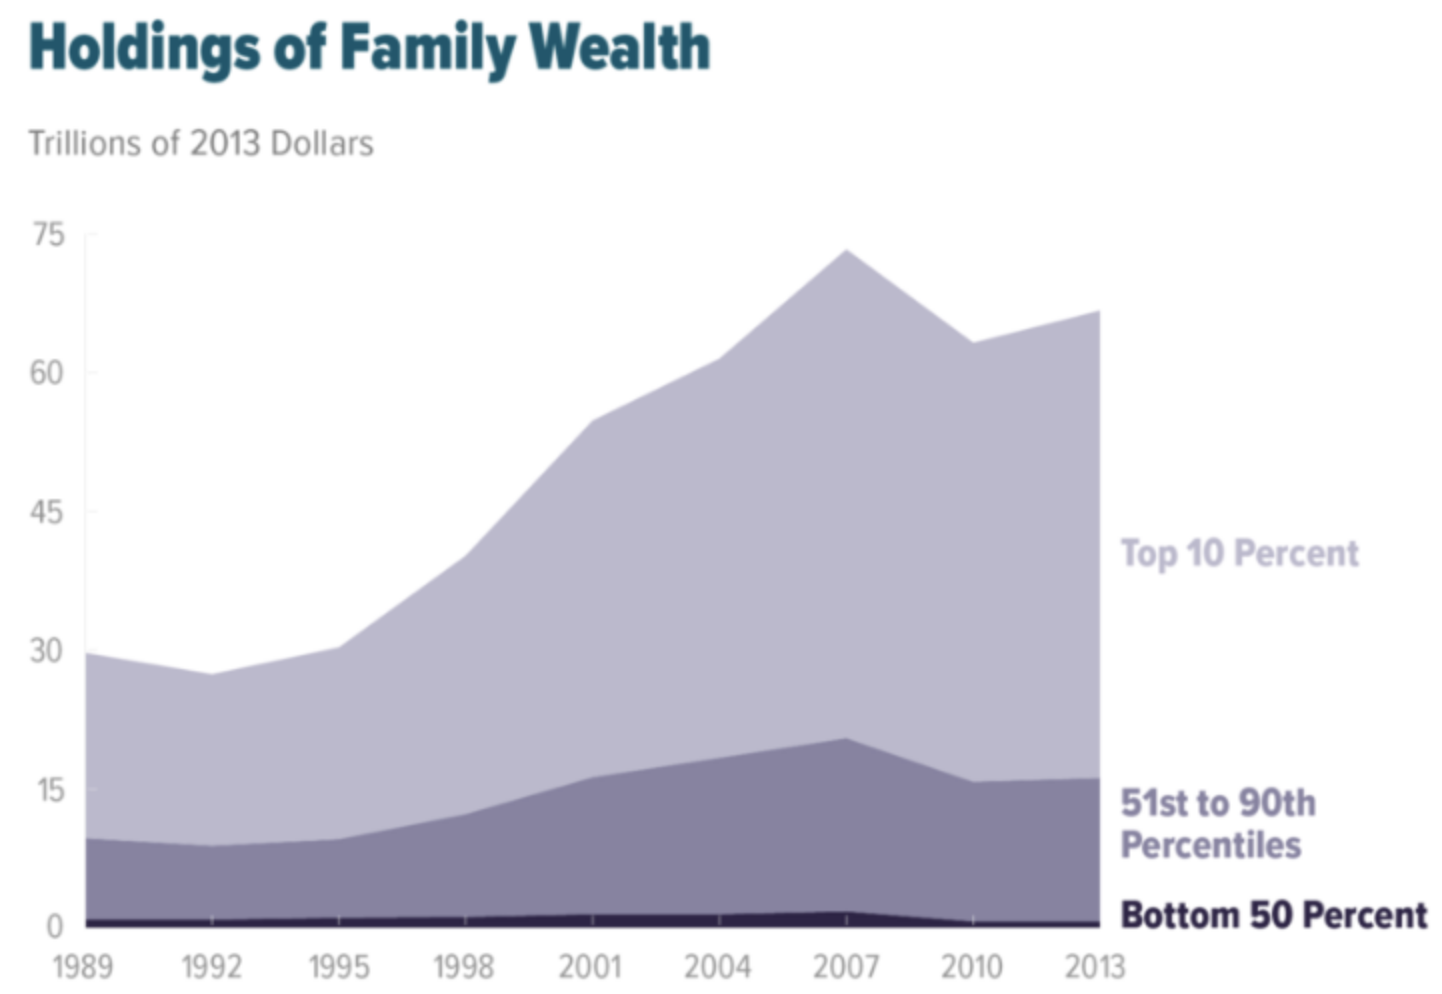
\includegraphics[scale=0.3]{inequality.png}
\end{center}
\end{column}
\end{columns}

\end{frame}

%@@@@@@@@@@@@@@@@@@@@@@@@@@@@@@@@@@@@@@@@@@@@@@@@@
\begin{frame}
\frametitle{Inequality}

\begin{columns}
\begin{column}{0.5\textwidth}

\begin{itemize}
\item When inequality goes up in a \textbf{community}:
\begin{itemize}
\item interpersonal trust goes down;
\item interpersonal hostility goes up;
\item violence goes up;
\item discrimination goes up;
\item civic and political participation goes down;
\end{itemize}
\bigskip
\bigskip
\item Income inequality undermines \textbf{democracy}:
\begin{itemize}
\item Selects out individuals from seeking office;
\item Responsiveness to wealthy interests;
\item Lobbying.
\end{itemize}
\end{itemize}
\end{column}

\begin{column}{0.5\textwidth}
\begin{center}
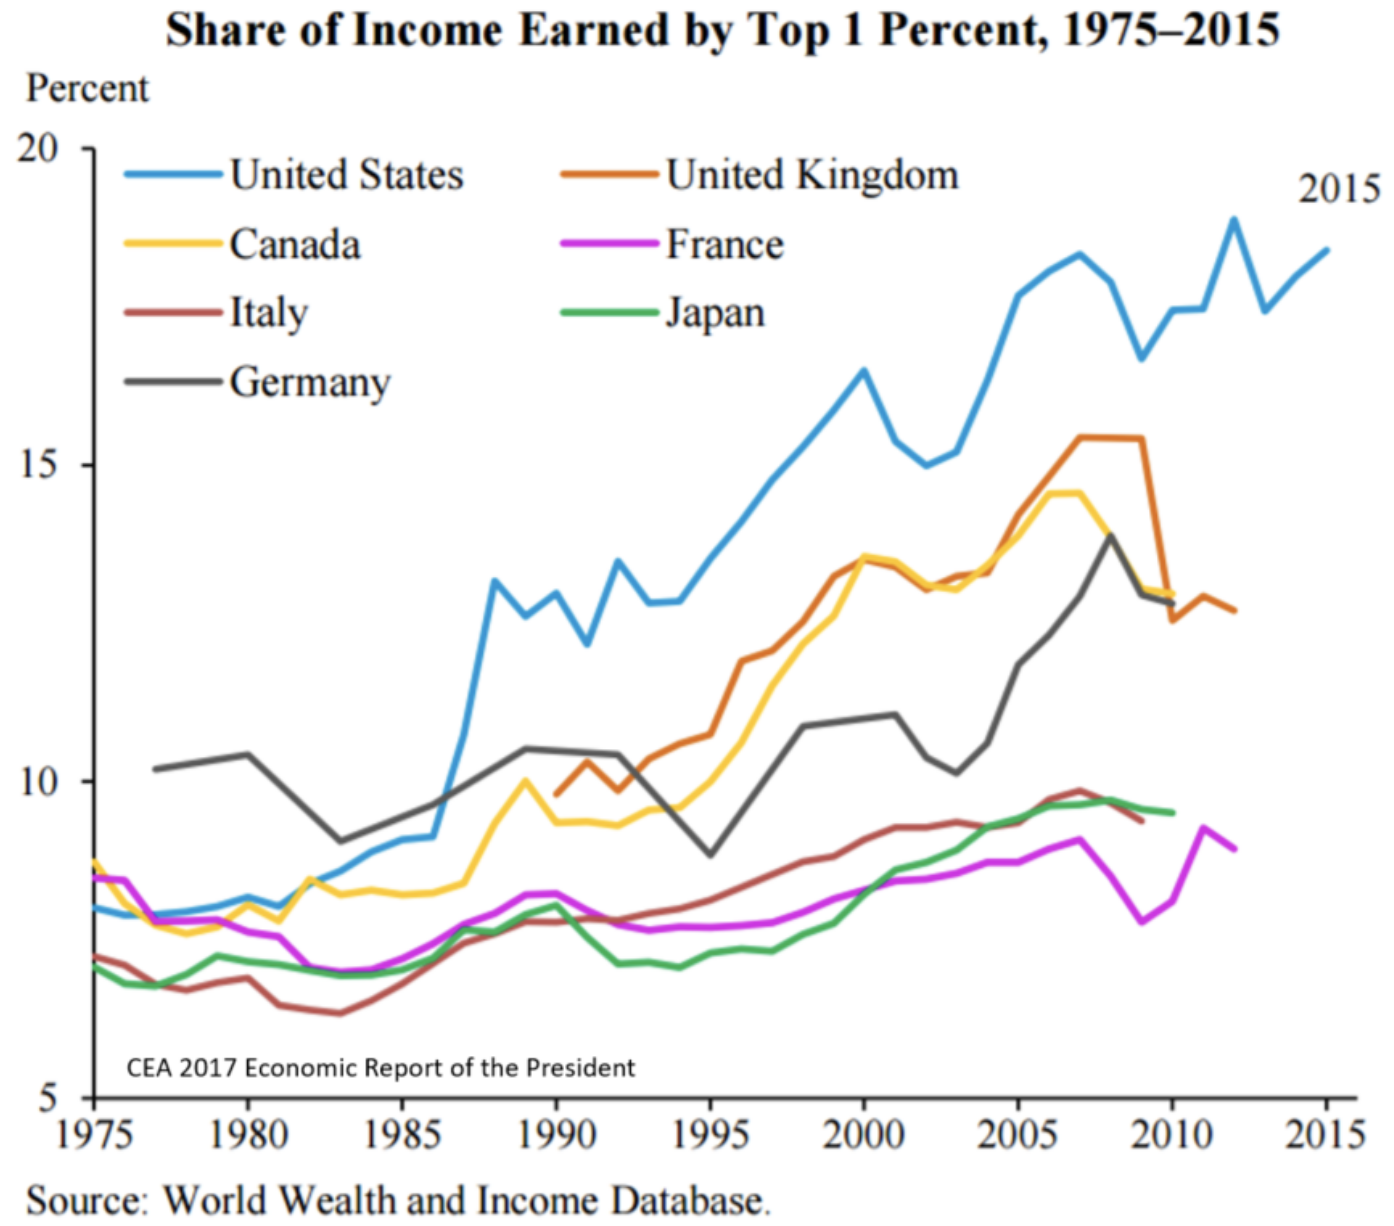
\includegraphics[scale=0.3]{inequality_2.png}
\end{center}
\end{column}
\end{columns}

\end{frame}

%@@@@@@@@@@@@@@@@@@@@@@@@@@@@@@@@@@@@@@@@@@@@@@@@@
\begin{frame}

\begin{center}
\Huge\textbf{Goals : Efficiency}\\
\bigskip
\bigskip
\large The ratio between input and output, effort and results, expenditure and income, or cost and benefit
\end{center}

\end{frame}

%@@@@@@@@@@@@@@@@@@@@@@@@@@@@@@@@@@@@@@@@@@@@@@@@@
\begin{frame}
\frametitle{Measurement}
\begin{itemize}
\item How do we measure efficiency (need to measure both inputs and outputs)?
\begin{itemize}
\item How to balance multiple objectives?
\item What if the value of a given output is multidimensional?
\item What if something is both input and output?
\item Do we count second and third order effects as outputs?
\item What do we do with opportunity costs?
\end{itemize}
\end{itemize}

\end{frame}

%@@@@@@@@@@@@@@@@@@@@@@@@@@@@@@@@@@@@@@@@@@@@@@@@@
\begin{frame}
\frametitle{Markets}
\begin{itemize}
\item \textbf{Theoretical}: markets w/ voluntary exchange maximize efficiency, social welfare;
\begin{itemize}
\item Voluntary exchange $=$ at least one actor better off and nobody worse off;
\item If actors optimize and social welfare $=$ their summed utility then it will be maximized;
\end{itemize}
\bigskip
\bigskip
\item \textbf{Corollary}: free markets can produce social welfare more effectively than governments;
\bigskip
\bigskip
\item Results on maximized social welfare are developed in the context of \textbf{full information} and \textbf{Voluntarism};
\begin{itemize}
\item In the Polis information revelation is strategic;
\item Welfare results can be extended in an ex ante sense to incomplete information environments;
\item Involuntary trade compromises efficiency and welfare; %(e.g. the labor/wage trade in a poor labor market);
\end{itemize}
\bigskip
\bigskip
\item Stone's critiques: many roles; interdependent welfare; ignores distribution; community goals.
\end{itemize}

\end{frame}

%@@@@@@@@@@@@@@@@@@@@@@@@@@@@@@@@@@@@@@@@@@@@@@@@@
\begin{frame}

\begin{center}
\Huge\textbf{Goals : Welfare}\\
\bigskip
\bigskip
\large Government is a contrivance of human wisdom to provide for human wants (Burke)
\end{center}

\end{frame}

%@@@@@@@@@@@@@@@@@@@@@@@@@@@@@@@@@@@@@@@@@@@@@@@@@
\begin{frame}
\frametitle{Dimensions of need:}
\begin{columns}
\begin{column}{0.5\textwidth}

\begin{itemize}
\item \textbf{Material/Symbolic} (e.g. food satisfies cultural need too);
\item \textbf{Intrinsic/Instrumental} (e.g. money is instrumental, freedom to choose is intrinsic);
\item \textbf{Volatility/Security} (e.g. minimize risk);
\item \textbf{Quantity/Quality} (e.g. how much longer you live vs how well you feel);
\item \textbf{Individual/Relational} (e.g. need to care for others);
\item \textbf{Absolute/Relative} (e.g. keeping up with the Joneses).
\end{itemize}
\end{column}
\begin{column}{0.5\textwidth}
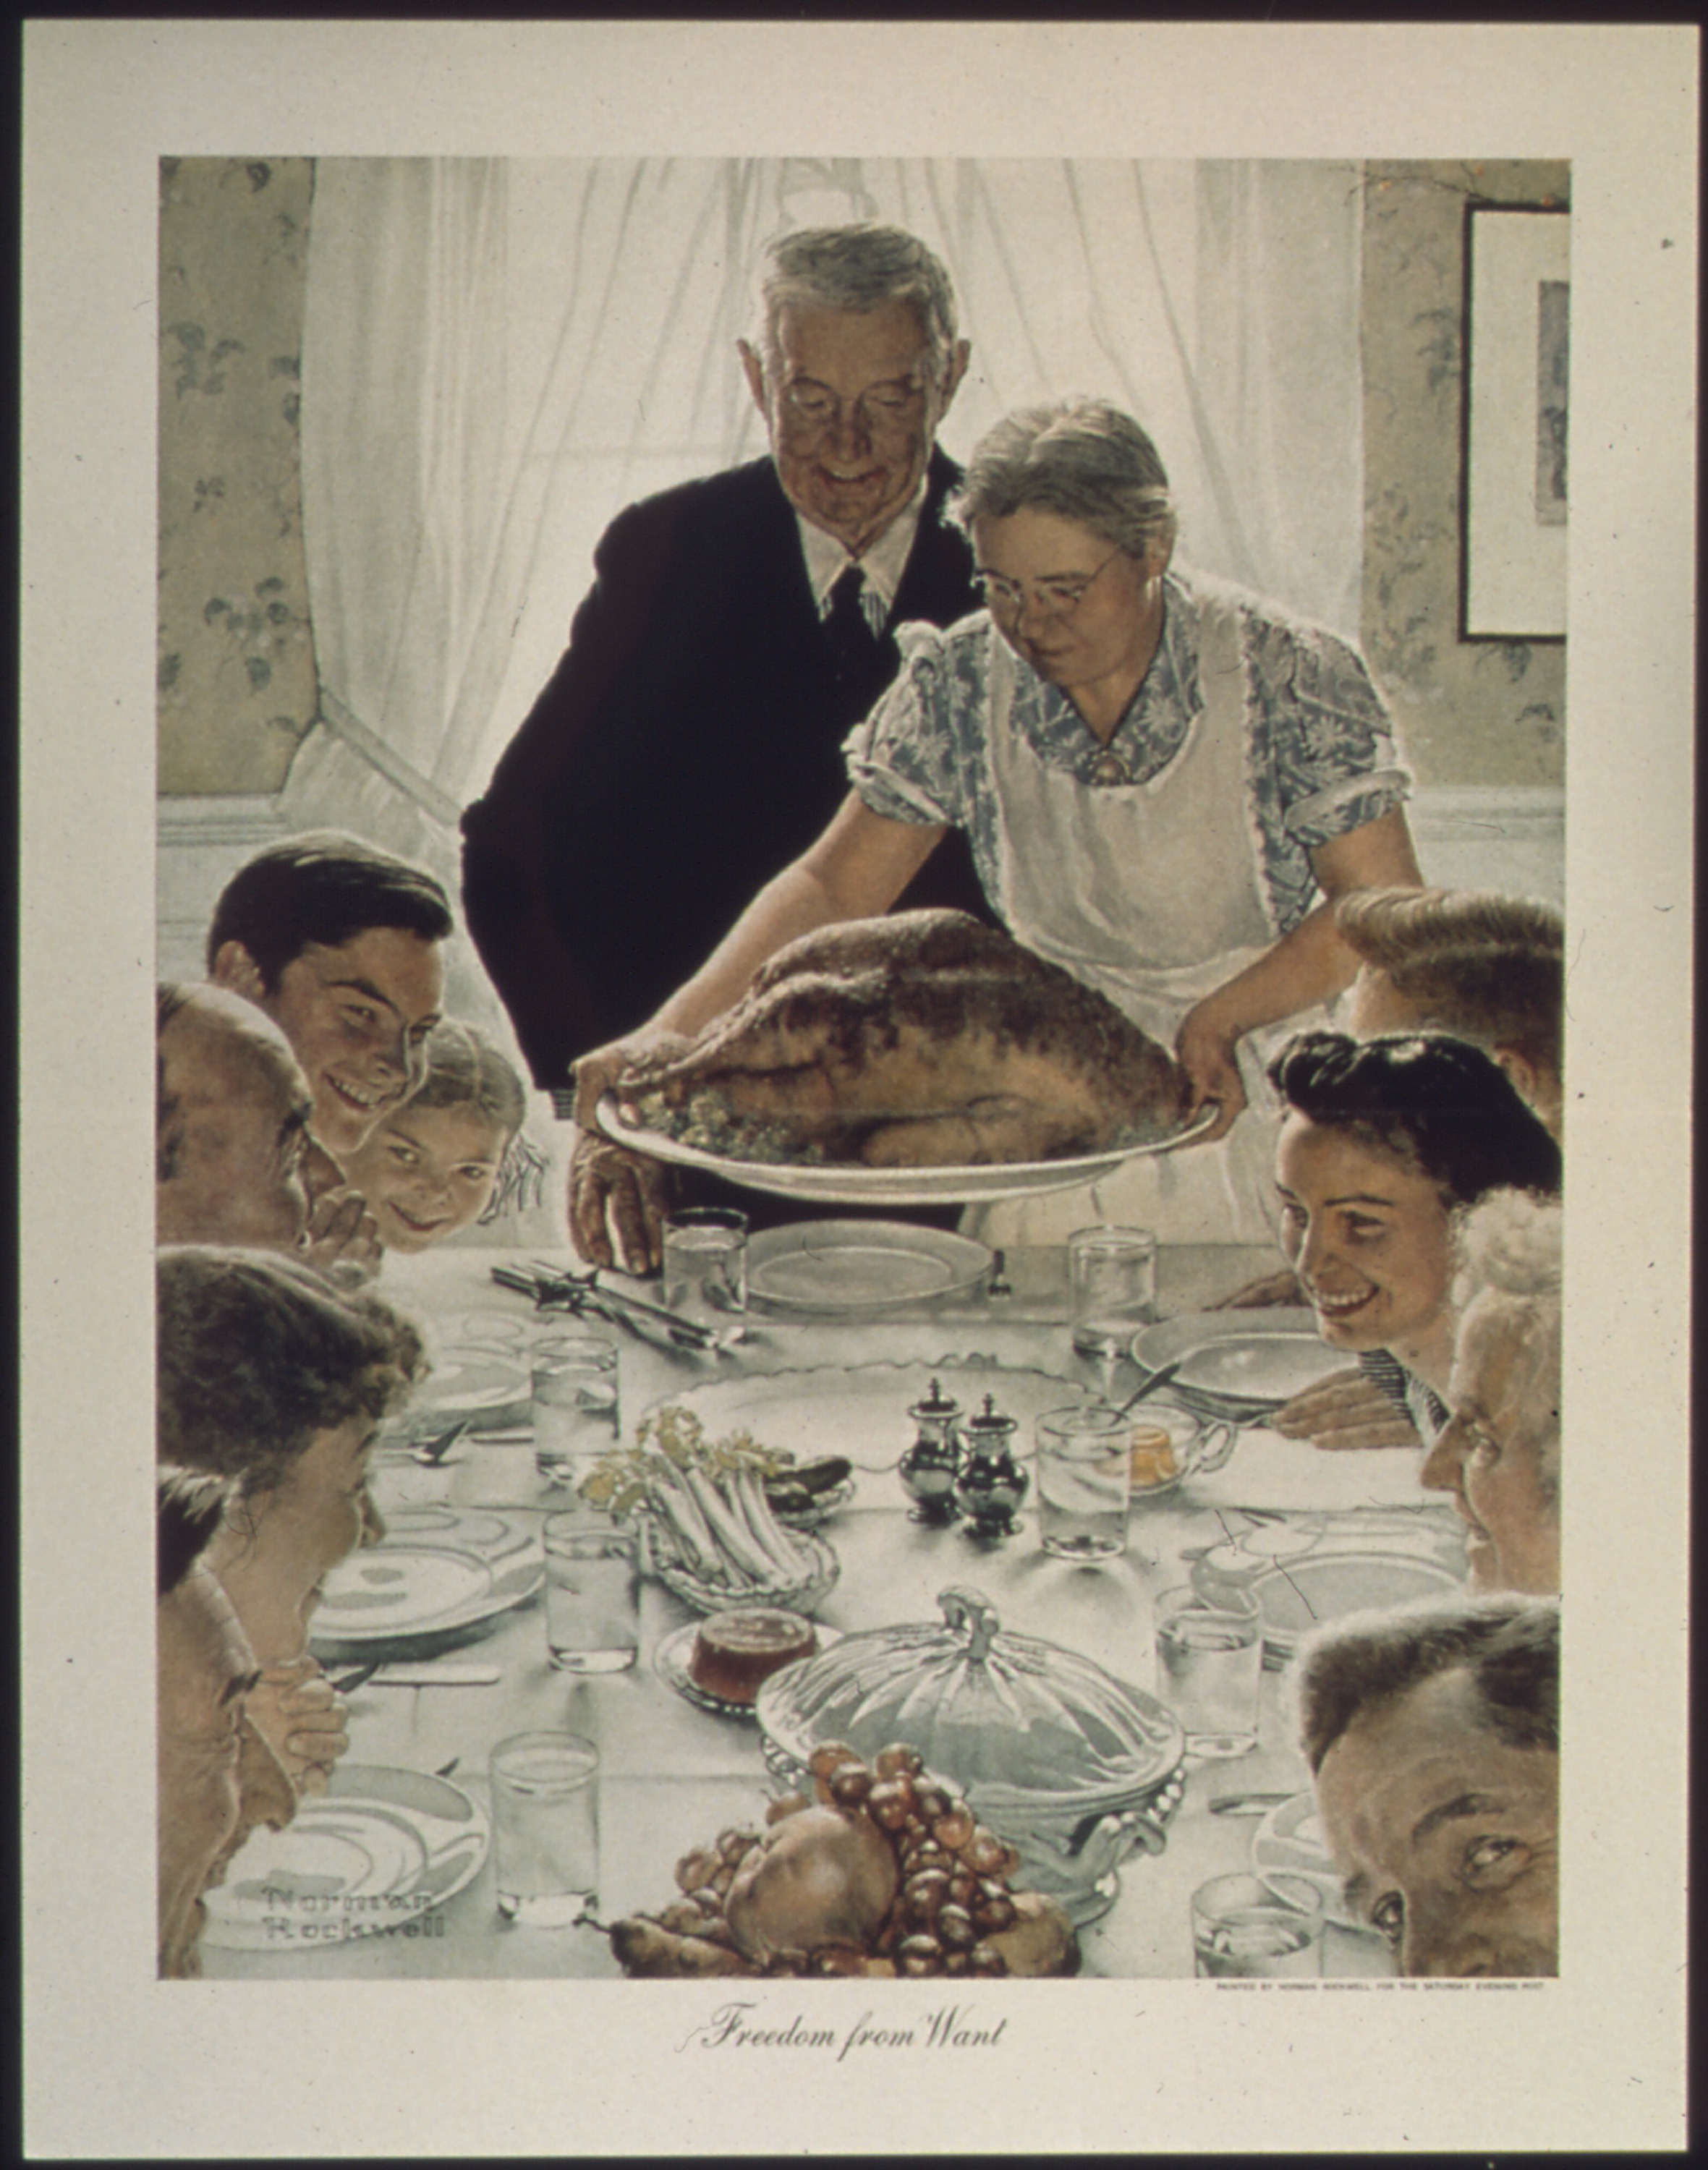
\includegraphics[scale=0.25]{Freedom_From_Want.jpg}
\end{column}
\end{columns}
\end{frame}

%@@@@@@@@@@@@@@@@@@@@@@@@@@@@@@@@@@@@@@@@@@@@@@@@@
\begin{frame}
\frametitle{Dimensions of need:}
\begin{columns}
\begin{column}{0.5\textwidth}

\begin{itemize}
\item \textbf{Material/Symbolic} (e.g. food satisfies cultural need too);
\item \textbf{Intrinsic/Instrumental} (e.g. money is instrumental, freedom to choose is intrinsic);
\item \textbf{Volatility/Security} (e.g. minimize risk);
\item \textbf{Quantity/Quality} (e.g. how much longer you live vs how well you feel);
\item \textbf{Individual/Relational} (e.g. need to care for others);
\item \textbf{Absolute/Relative} (e.g. keeping up with the Joneses).
\end{itemize}
\end{column}
\begin{column}{0.5\textwidth}
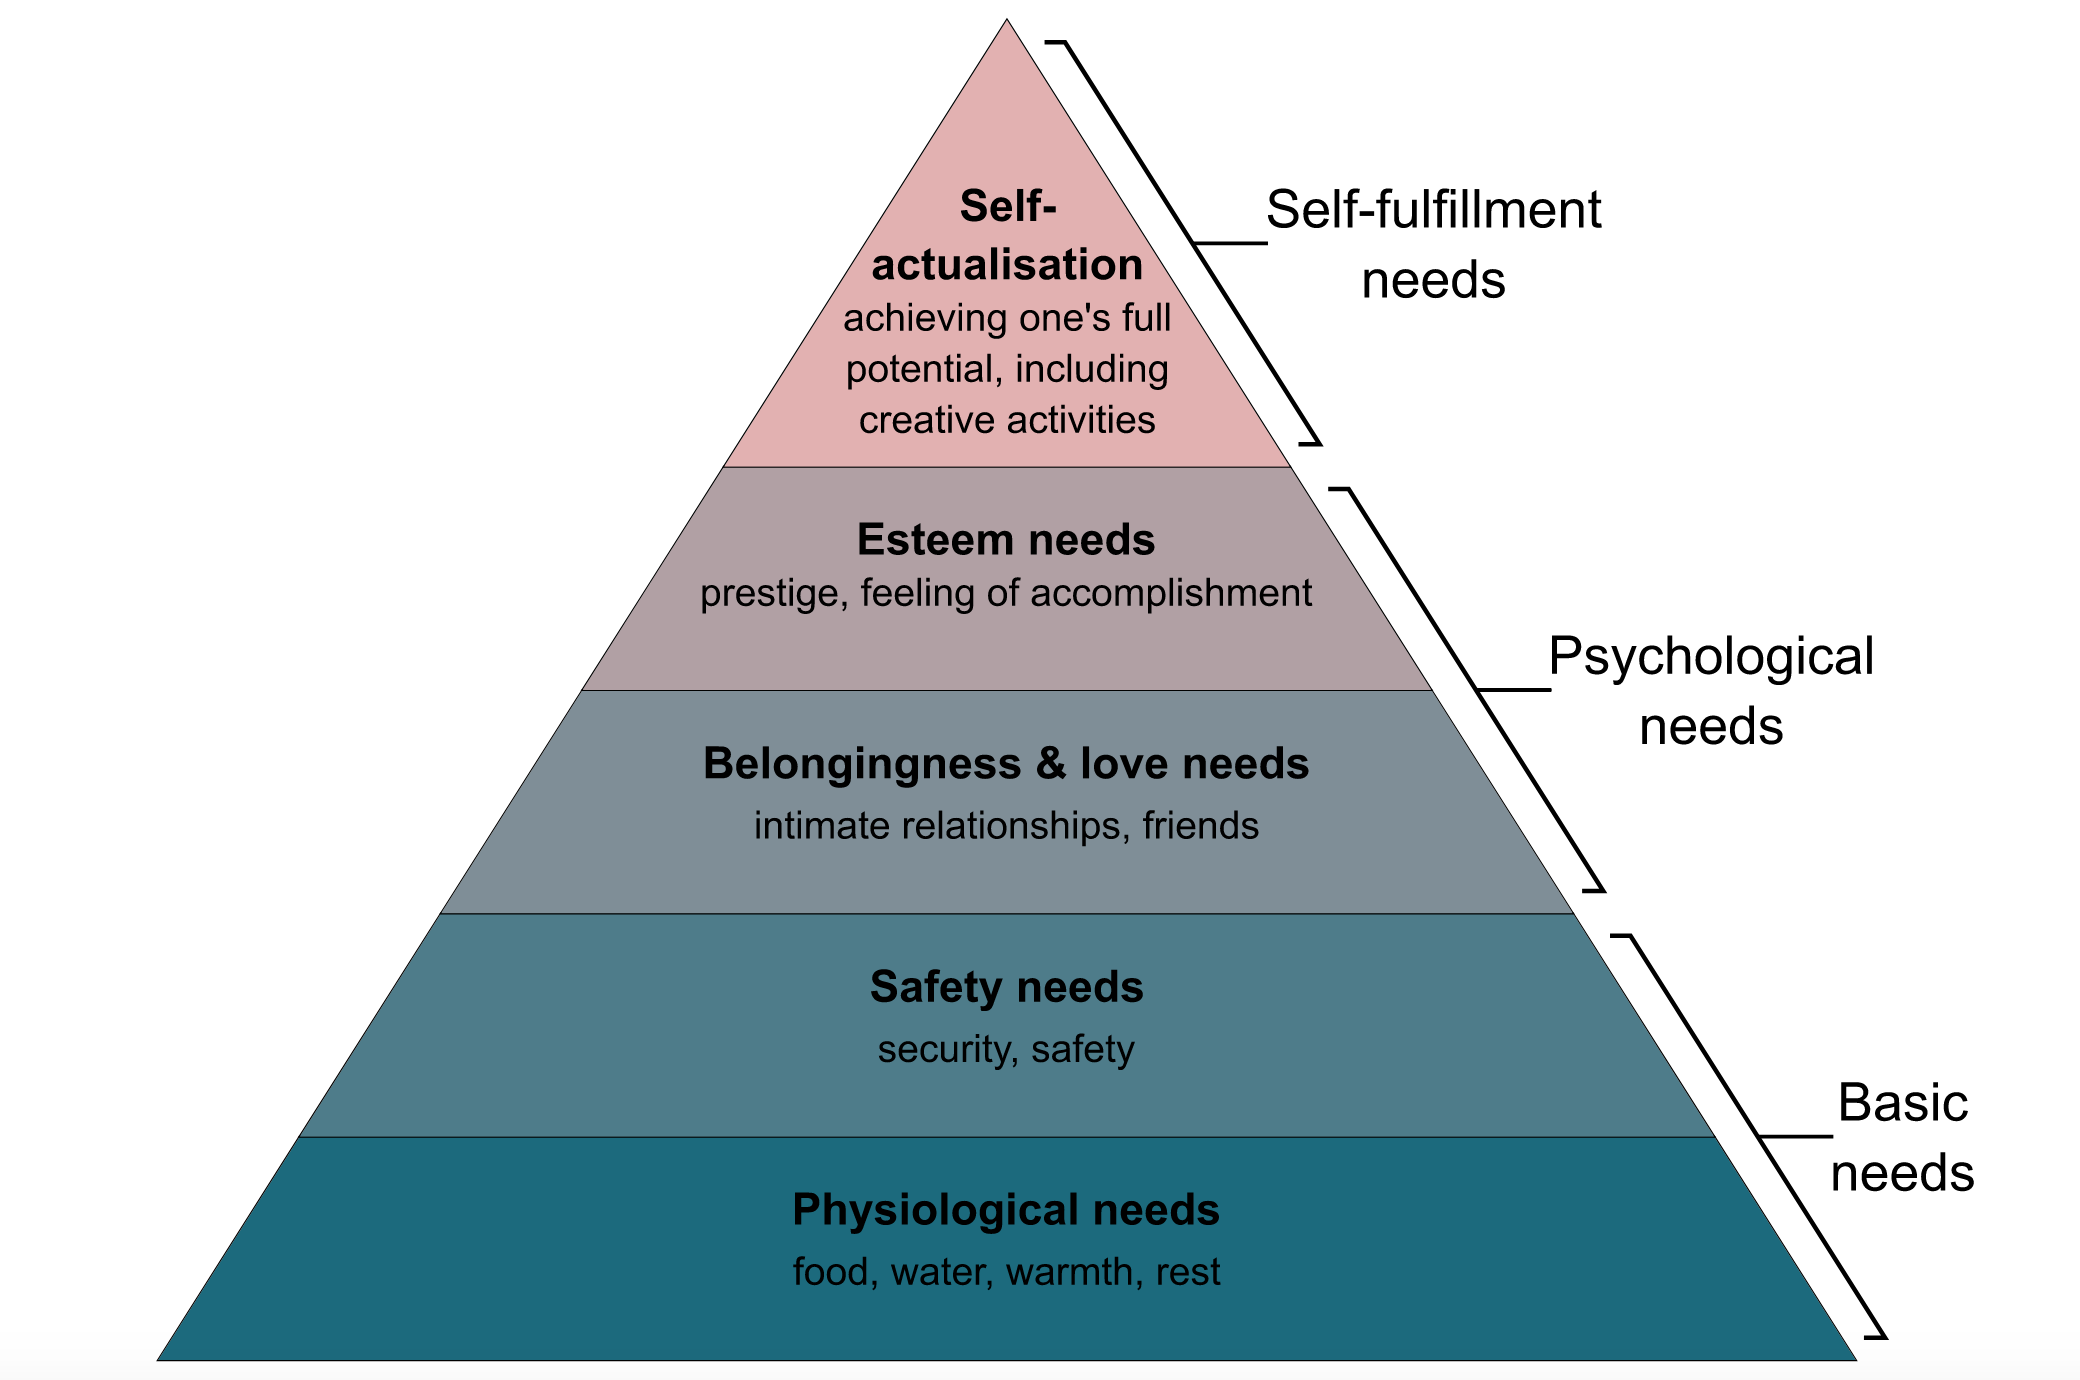
\includegraphics[scale=0.2]{maslow.png}
\end{column}
\end{columns}
\end{frame}

%@@@@@@@@@@@@@@@@@@@@@@@@@@@@@@@@@@@@@@@@@@@@@@@@@
\begin{frame}
\frametitle{Moral Hazard}
\begin{columns}
\begin{column}{0.5\textwidth}

\begin{itemize}
\item \textbf{Moral hazard}: an entity has an incentive to increase its exposure to risk when it does not bear the full costs of that risk;
\begin{itemize}
\item post-contract shifts in optimal choice;
\item information asymmetry;
\item principal-agent problems;
\end{itemize}
\bigskip
\item Originally from insurance (from back in the 18th century!);
\end{itemize}
\end{column}
\begin{column}{0.5\textwidth}
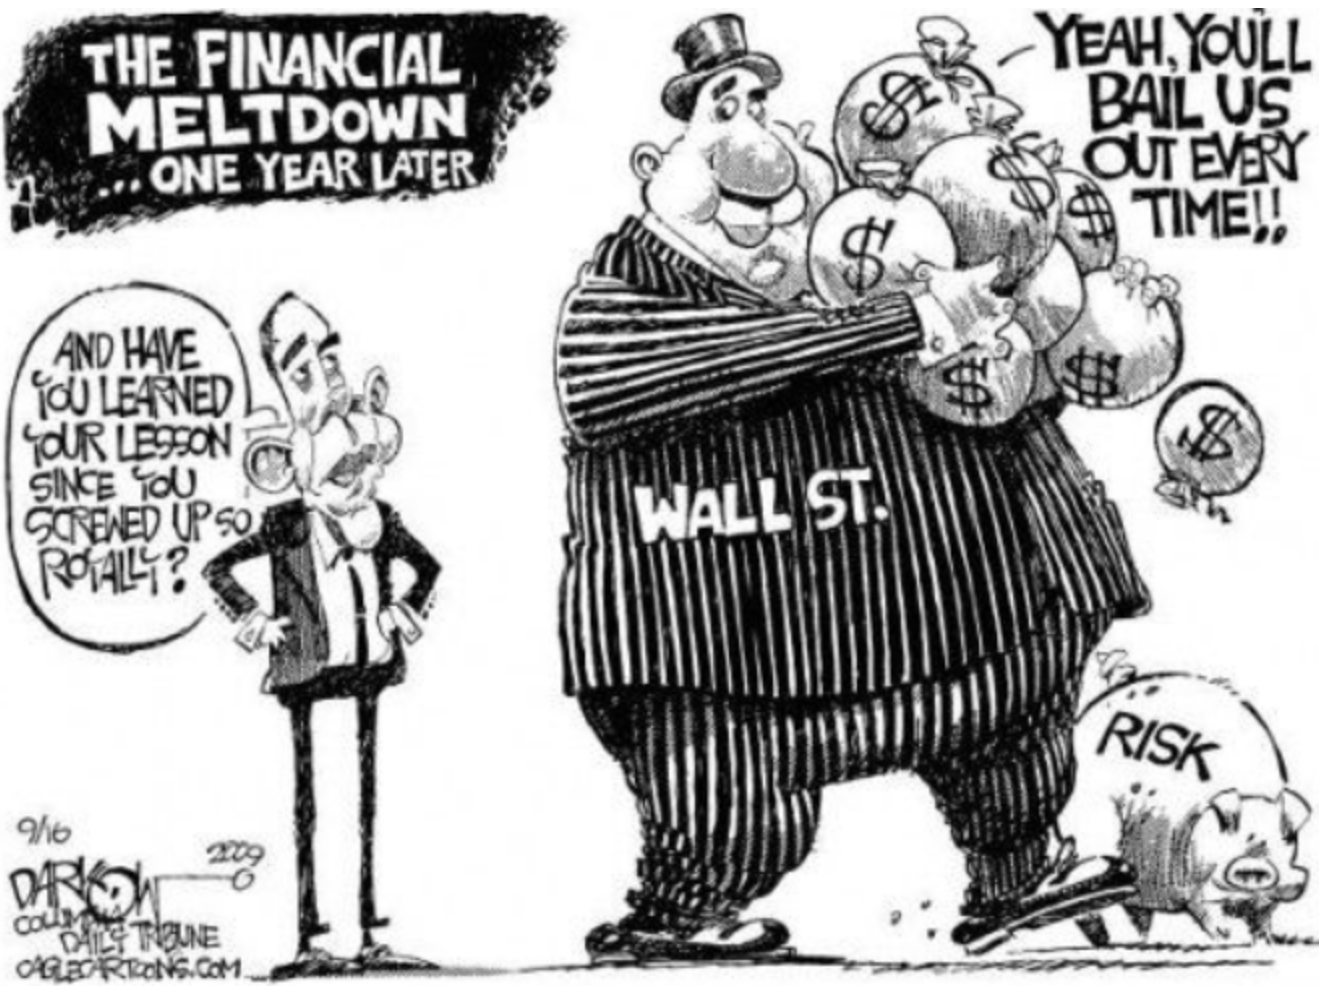
\includegraphics[scale=0.3]{moral_hazard.png}
\end{column}
\end{columns}
\end{frame}

%@@@@@@@@@@@@@@@@@@@@@@@@@@@@@@@@@@@@@@@@@@@@@@@@@
\begin{frame}

\begin{center}
\Huge\textbf{Goals : Liberty}\\
\bigskip
\bigskip
\large Unconstrained choice
\end{center}

\end{frame}

%@@@@@@@@@@@@@@@@@@@@@@@@@@@@@@@@@@@@@@@@@@@@@@@@@
\begin{frame}
\frametitle{Questions:}
\begin{itemize}
\item When can government legitimately interfere w/ citizens' choices and activities?
\bigskip
\bigskip
\item When should community goals supersede individual choice? 
\bigskip
\bigskip
\item Under what circumstances should public policy limit individual autonomy?
\end{itemize}

\end{frame}

%@@@@@@@@@@@@@@@@@@@@@@@@@@@@@@@@@@@@@@@@@@@@@@@@@
\begin{frame}
\frametitle{Answer:}
\begin{columns}
\begin{column}{0.5\textwidth}

\begin{quote}
The sole end for which mankind are warranted, individually or collectively, in interfering with the liberty of action of any of their number is self-protection...[T]he only purpose for which power can he rightfully exercised over any member of a civilized community, against his will, is to prevent harm to others.\\
\hspace{25mm}$\sim$ John Stuart Mill
\end{quote}
\end{column}
\begin{column}{0.5\textwidth}
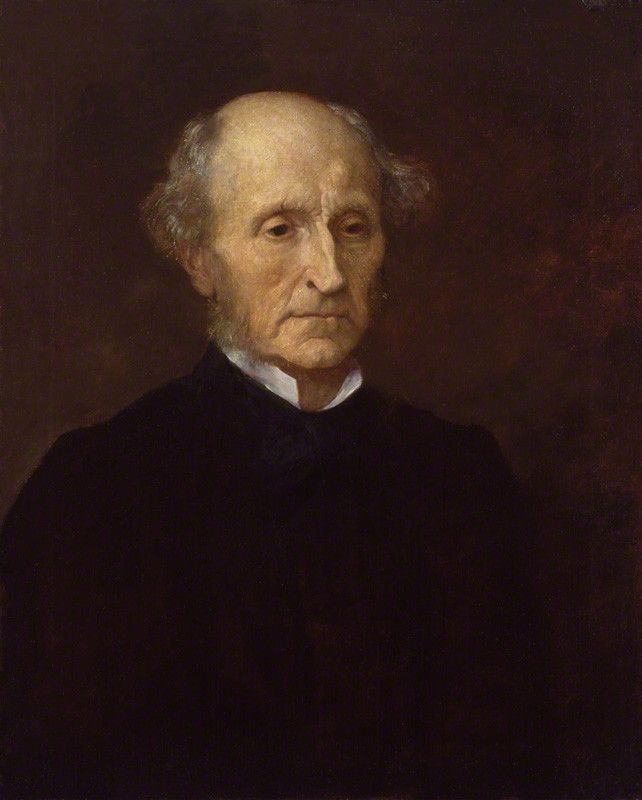
\includegraphics[scale=0.25]{JSM.jpg}
\end{column}
\end{columns}
\end{frame}

%@@@@@@@@@@@@@@@@@@@@@@@@@@@@@@@@@@@@@@@@@@@@@@@@@
\begin{frame}
\frametitle{what counts as `harm' to others?}
\begin{itemize}
\item Mill: physical injury caused to another;
\bigskip
\bigskip
\item In commons problems (e.g. private gains mean public costs) how to apply this?
\begin{itemize}
\item Grains of sugar thought experiment;
\item Who is to be regulated in group situations?
\end{itemize}
\bigskip
\bigskip
\item Other harms -- recognition of these is a matter of political struggle:
\begin{itemize}
\item Economic and material;
\item Aesthetic;
\item Psychic (e.g. worry);
\item Spiritual/moral.
\end{itemize}
\end{itemize}

\end{frame}

%@@@@@@@@@@@@@@@@@@@@@@@@@@@@@@@@@@@@@@@@@@@@@@@@@
\begin{frame}
\frametitle{Positive/Negative liberty}
\begin{itemize}
\item \textbf{Negative liberty}: ``I am free to the extent that no one interferes with my activity."
\begin{itemize}
\item Coercion $=$ taking the resources of another;
\item ``Those who are taxed without their own consent are slaves."
\end{itemize}
\bigskip
\bigskip
\item \textbf{Positive liberty}: ``I am free to the extent that I can choose my life path."
\begin{itemize}
\item Coercion $=$ significant deprivation relative to status quo;
\item Health care, nutrition, shelter, and political power are essential for exercising freedom (Sen);
\end{itemize}
\end{itemize}

\end{frame}



%@@@@@@@@@@@@@@@@@@@@@@@@@@@@@@@@@@@@@@@@@@@@@@@@@
\begin{frame}

\begin{center}
\Huge\textbf{Goals : Security}\\
\end{center}

\end{frame}

%@@@@@@@@@@@@@@@@@@@@@@@@@@@@@@@@@@@@@@@@@@@@@@@@@
\begin{frame}
\frametitle{Three concepts of security}
\begin{columns}
\begin{column}{0.5\textwidth}
\begin{itemize}
\item Absence of worry (Rockwell);
\bigskip
\bigskip
\bigskip
\item Good policy (Roosevelt);
\bigskip
\bigskip
\bigskip
\item Scientific risk mitigation (expected values);
\end{itemize}
\end{column}
\begin{column}{0.5\textwidth}
\includegraphics[scale=0.25]{Freedom_From_Fear.jpg}
\end{column}
\end{columns}

\end{frame}

%@@@@@@@@@@@@@@@@@@@@@@@@@@@@@@@@@@@@@@@@@@@@@@@@@
\begin{frame}
\frametitle{Risk analysis and Expected Value}
\begin{itemize}
\item \textbf{Expected value} $=$ weighting the value of each outcome by the likelihood that it happens;
\begin{itemize}
\item Gambling: suppose w/ probability $0.75$ you win \$10, w/ probability $0.15$ you win \$5, w/ probability $0.1$ you lose \$10.  Then expected value is:
\begin{align*}
0.75*10 + 0.15*5 + 0.1*(-10) = \mbox{\$}7.25;
\end{align*}
\item Strong axiomatic reasons to use (e.g. Von Neumann-Morgenstern Utility Theorem);
\end{itemize}
\bigskip
\bigskip
\bigskip
\item Widely used (in much more general forms) in economics and mathematics;
\end{itemize}
\end{frame}

%@@@@@@@@@@@@@@@@@@@@@@@@@@@@@@@@@@@@@@@@@@@@@@@@@
\begin{frame}
\frametitle{Criticism of Expected Value}
\begin{itemize}
\item Expected value $\neq$ psychological security -- requires agenda setting (e.g. cholesterol);
\bigskip
\bigskip
\item An event is less bad if it isn't certain to occur;
\begin{itemize}
\item If an event would be absolutely catastrophic but highly unlikely to occur, it would count for almost nothing in the analysis;
\item Not clear why this is problematic -- should something become \textit{more} impactful if less likely?
\end{itemize}
\bigskip
\bigskip
\item Expected value isn't the way people experience insecurity:
\begin{itemize}
\item Before: doesn't account for imagination (why can't you just add more terms?);
\item After: Actual outcome does not equal expected value (irrelevant as long as it is one of the possibilities);
\end{itemize}
\bigskip
\bigskip
\item More compelling -- results from experimental economics:
\begin{itemize}
\item Ellsberg paradox: choices violate predictions of expected utility;
\item Allais paradox: axiom of rationality (Independence) may be violated.
\end{itemize}
\end{itemize}
\end{frame}

%@@@@@@@@@@@@@@@@@@@@@@@@@@@@@@@@@@@@@@@@@@@@@@@@@
\begin{frame}
\frametitle{Security in the Polis}
\begin{columns}
\begin{column}{0.5\textwidth}

\begin{itemize}
\item Threat prevention;
\bigskip
\bigskip
\bigskip
\item Harm mitigation;
\bigskip
\bigskip
\bigskip
\item Reassurance;
\begin{itemize}
\item Project control;
\item Absolute characterizations;
\item Decisive action (e.g. Cheney's one percent criterion).
\end{itemize}
\end{itemize}
\end{column}
\begin{column}{0.5\textwidth}
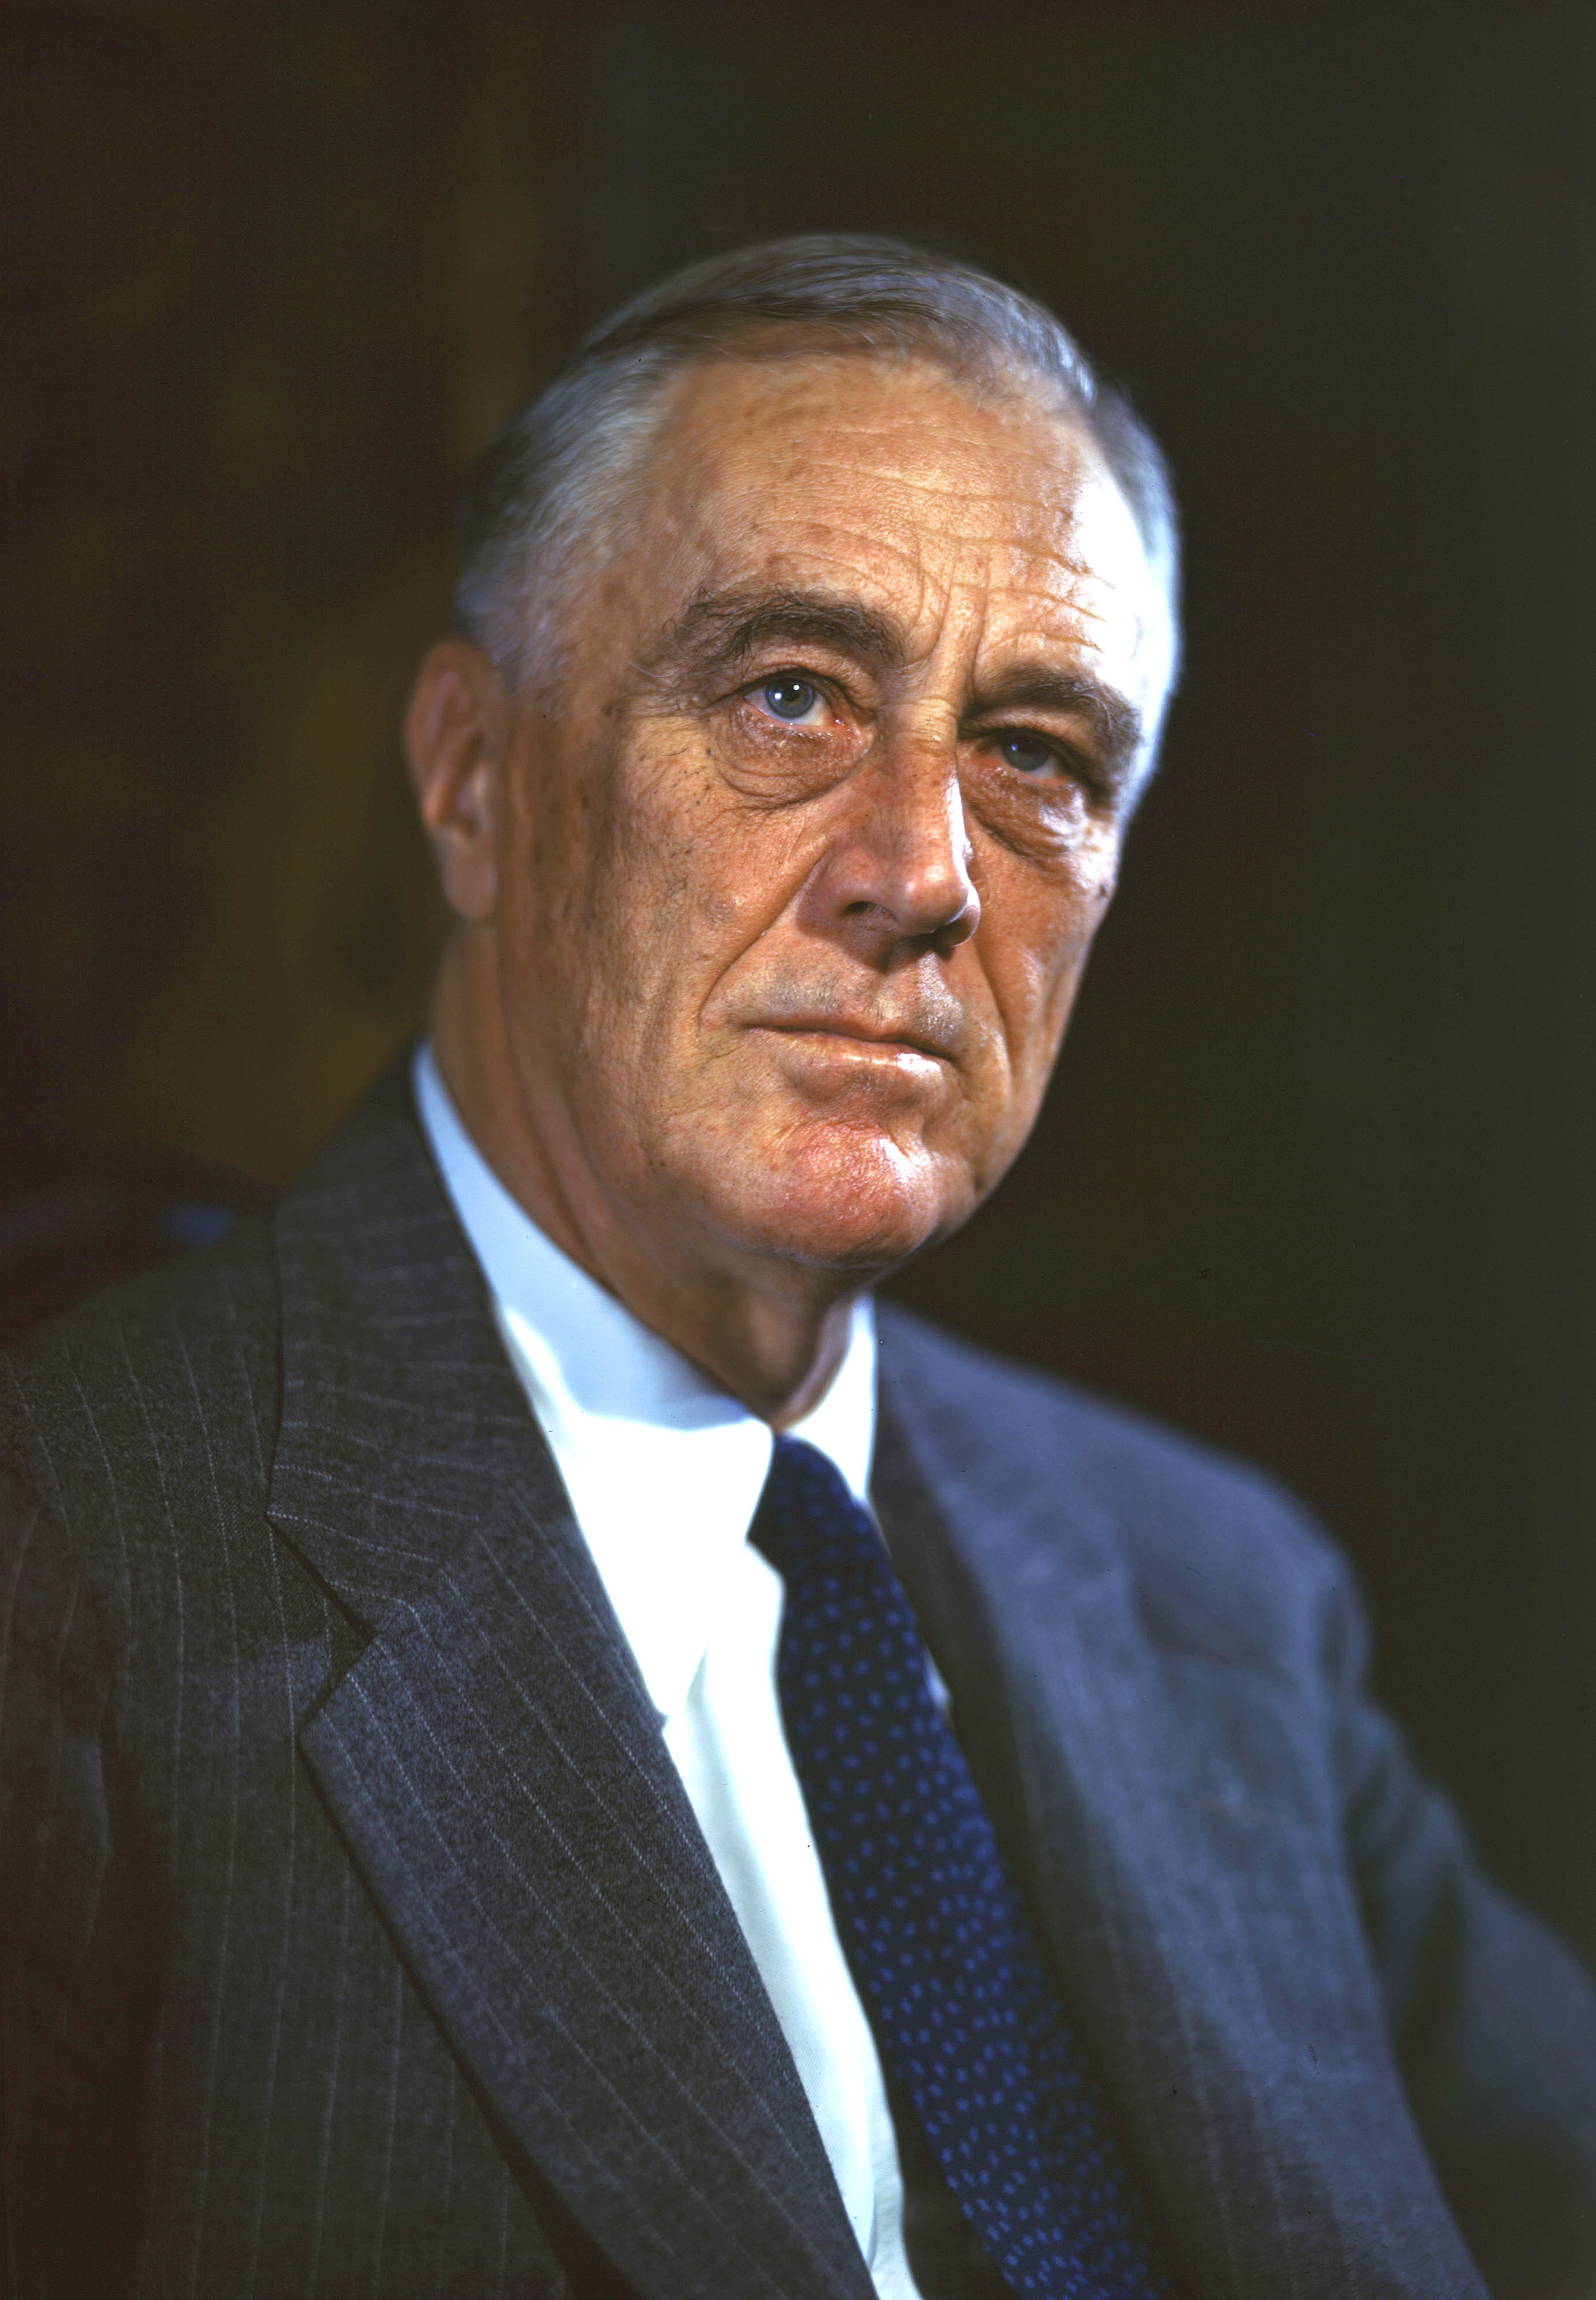
\includegraphics[scale=0.05]{FDR.jpg}
\end{column}
\end{columns}

\end{frame}

%%@@@@@@@@@@@@@@@@@@@@@@@@@@@@@@@@@@@@@@@@@@@@@@@@@
%\begin{frame}
%\frametitle{What makes risks ok?}
%\begin{itemize}
%\item When two catastrophes have the same expected value rational people should care about them equally... but they often prefer that government addresses one over another;
%\bigskip
%\bigskip
%\bigskip
%\item Factors that influence views on different sources of risk
%\begin{itemize}
%\item Accidental side effect vs intentional choice (e.g. stupidity vs malice);
%\item Form of risk (nuclear vs terrorist);
%\item Familiarity;
%\item Equity.
%\end{itemize}
%\end{itemize}
%\end{frame}



%@@@@@@@@@@@@@@@@@@@@@@@@@@@@@@@@@@@@@@@@@@@@@@@@@
\begin{frame}

\begin{center}
\Huge\textbf{Are there tradeoffs?}
\end{center}

\end{frame}

%@@@@@@@@@@@@@@@@@@@@@@@@@@@@@@@@@@@@@@@@@@@@@@@@@
\begin{frame}
\frametitle{Equality-Efficiency Tradeoffs}
\begin{itemize}
\item Argument: equality seeking policy (e.g. redistribution) compromise efficiency and thereby social welfare;
\begin{itemize}
\item Inequality promotes productivity;
\item Redistribution is administratively costly;
\end{itemize}
\bigskip
\bigskip
\item Empirical evidence is mixed.
\end{itemize}

\end{frame}

%@@@@@@@@@@@@@@@@@@@@@@@@@@@@@@@@@@@@@@@@@@@@@@@@@
\begin{frame}
\frametitle{Welfare--Efficiency Tradeoffs}

\begin{itemize}
\item Moral hazard arguments can be used to suggest a tradeoff:
\begin{itemize}
\item Welfare policy $=$ meeting needs without work; 
\item Recipients will work less as will providers; 
\item Total productivity will go down;
\end{itemize}
\bigskip
\bigskip
\item Theoretical: how to square distaste for risk with welfare--efficiency tradeoff?
\bigskip
\bigskip
\item Empirical: sketchy support in the data (e.g. NJ negative income tax, cross national employment comparisons, consumption of medical care).
\end{itemize}

\end{frame}

%@@@@@@@@@@@@@@@@@@@@@@@@@@@@@@@@@@@@@@@@@@@@@@@@@
\begin{frame}
\frametitle{Liberty Tradeoffs}
\begin{itemize}
\item Liberty--Equality Tradeoff
\begin{itemize}
\item Redistribution creates equality (in resources) but costs liberty for the advantaged;
\item Tradeoff is clear under the negative conception of liberty;
\item Stone: Under the positive conception of liberty a society that maximizes equality of wealth, health, knowledge, and power also equalizes its citizens' freedom to choose their life plans. Liberty and equality are not in a trade-off (maximize equality of wealth without limiting life plan choice for the advantaged?);
\end{itemize}
\bigskip
\bigskip
\item Liberty--Welfare Tradeoff
\begin{itemize}
\item Help = dependence;
\item Formal rights may not help much when power dynamics favor one side.
\end{itemize}
\end{itemize}

\end{frame}

%@@@@@@@@@@@@@@@@@@@@@@@@@@@@@@@@@@@@@@@@@@@@@@@@@
\begin{frame}
\frametitle{Security Tradeoffs}
\begin{itemize}
\item Liberty--Security Tradeoff
\begin{itemize}
\item Maximizing security requires restrictions on individual liberty;
\item e.g. the Patriot Act/war on terror, suspension of Habeas Corpus;
\end{itemize}
\bigskip
\bigskip
\item Efficiency--Security Tradeoff
\begin{itemize}
\item Guns vs butter.
\end{itemize}
\end{itemize}

\end{frame}

%@@@@@@@@@@@@@@@@@@@@@@@@@@@@@@@@@@@@@@@@@@@@@@@@@
\begin{frame}

\begin{center}
\Huge\textbf{Why should we care?}\\
\bigskip
\bigskip
\large If there are tradeoffs then increasing one goal means decreasing another -- will exacerbate conflict caused by $v\neq w$:
\begin{align*}
w_{1}*\mbox{Equity} + w_2*\mbox{Efficiency} + w_3*\mbox{Welfare} + w_4*\mbox{Liberty} + w_5*\mbox{Security}\\
v_{1}*\mbox{Equity} + v_2*\mbox{Efficiency} + v_3*\mbox{Welfare} + v_4*\mbox{Liberty} + v_5*\mbox{Security}.
\end{align*}
\end{center}

\end{frame}

%@@@@@@@@@@@@@@@@@@@@@@@@@@@@@@@@@@@@@@@@@@@@@@@@@
\begin{frame}

\begin{center}
\Huge\textbf{Why should we care?}\\
\bigskip
\bigskip
\large Many policies aim at mitigating risk of harm (e.g. the what would happen if we didn't act question).  Understanding how to produce security and what makes risk acceptable enables policy makers to manipulate support for their policies.
\end{center}

\end{frame}

%@@@@@@@@@@@@@@@@@@@@@@@@@@@@@@@@@@@@@@@@@@@@@@@@@
\begin{frame}
\frametitle{Birkland$+$ Model of Policy}
\begin{itemize}
\item Policy Domain: what substantive problems are under consideration?  This specifies:
\begin{itemize}
\item The actors involved, official actors who can make decisions $+$ stakeholders; 
\item Distribution of benefits/costs $\Rightarrow$ actor organization, e.g. iron triangle, policy community;
\item The systemic agenda; 
\end{itemize}
\bigskip
\item \color{black}Input-output Model;
\begin{itemize}
\item Actors: legislature, executive, bureaucrats, justices and the available levers;
\item Inputs: agenda setting (application of power/social construction, focusing events, indicator change driven esp by unofficial actors) \textbf{sets goals}, determines the causal model, which specifies the institutional agenda, and leads to the policies on the decision agenda;
\item Black box decision making, timing (incrementalism, punctuated eq) driven by indicators/focusing events, choice driven by e.g. median voter thm, Arrow's thm;
\begin{itemize}
\item Round 1: works on decision agenda, leads to outputs (e.g. statute laws, rules, court decisions);
\item Round 2: Implementation, leads to outcomes;
 \end{itemize}
\end{itemize}
\bigskip
\item Outcomes: Feedback from failure and success, learning leads to iteration and updates.
\end{itemize}
\end{frame}

%@@@@@@@@@@@@@@@@@@@@@@@@@@@@@@@@@@@@@@@@@@@@@@@@@
\begin{frame}

\begin{center}
\Huge\textbf{Problems : Symbols}\\
\bigskip
\bigskip
\large Something that stands for something else -- tell stories that define policy problems.
\end{center}
\end{frame}

%%@@@@@@@@@@@@@@@@@@@@@@@@@@@@@@@@@@@@@@@@@@@@@@@@@
%\begin{frame}
%\frametitle{Why should we care about symbols?}
%\begin{columns}
%\begin{column}{0.5\textwidth}
%
%\begin{itemize}
%\item Symbols tell stories:
%\begin{itemize}
%\item Nooses $=$ racial hierarchy;
%\item Iraqi prison key $=$ progress;
%\item Face mask $=$ deference to science;
%\item Welfare queen $=$ inefficiency of the welfare state;
%\end{itemize}
%\bigskip
%\item Stories $=$ tools for defining policy problems;
%\bigskip
%\bigskip
%\item Stories imply causality.
%\end{itemize}
%\end{column}
%\begin{column}{0.5\textwidth}
%
\includegraphics[scale=1]{iraq_key.jpg}
%\end{column}
%\end{columns}
%
%\end{frame}

%@@@@@@@@@@@@@@@@@@@@@@@@@@@@@@@@@@@@@@@@@@@@@@@@@
\begin{frame}
\frametitle{Stories of Change}
\begin{columns}
\begin{column}{0.5\textwidth}

\begin{itemize}
\item Two variations, \textbf{rising} and \textbf{declining}:
\begin{itemize}
\item Rising: things are becoming more favorable (e.g. post Communist Poland);
\item Declining: things are becoming less favorable (e.g. post WWI Britain);
\end{itemize}
\bigskip
\item Perhaps correlated with development:
\begin{itemize}
\item Developed countries' progress is past;
\item Developing countries current experience is material and technological progress;
\end{itemize}
\bigskip
\item `Change is only an illusion' -- (e.g. Why Most Published Research Findings Are False, Ioannidis 2005).
\end{itemize}

\end{column}
\begin{column}{0.5\textwidth}
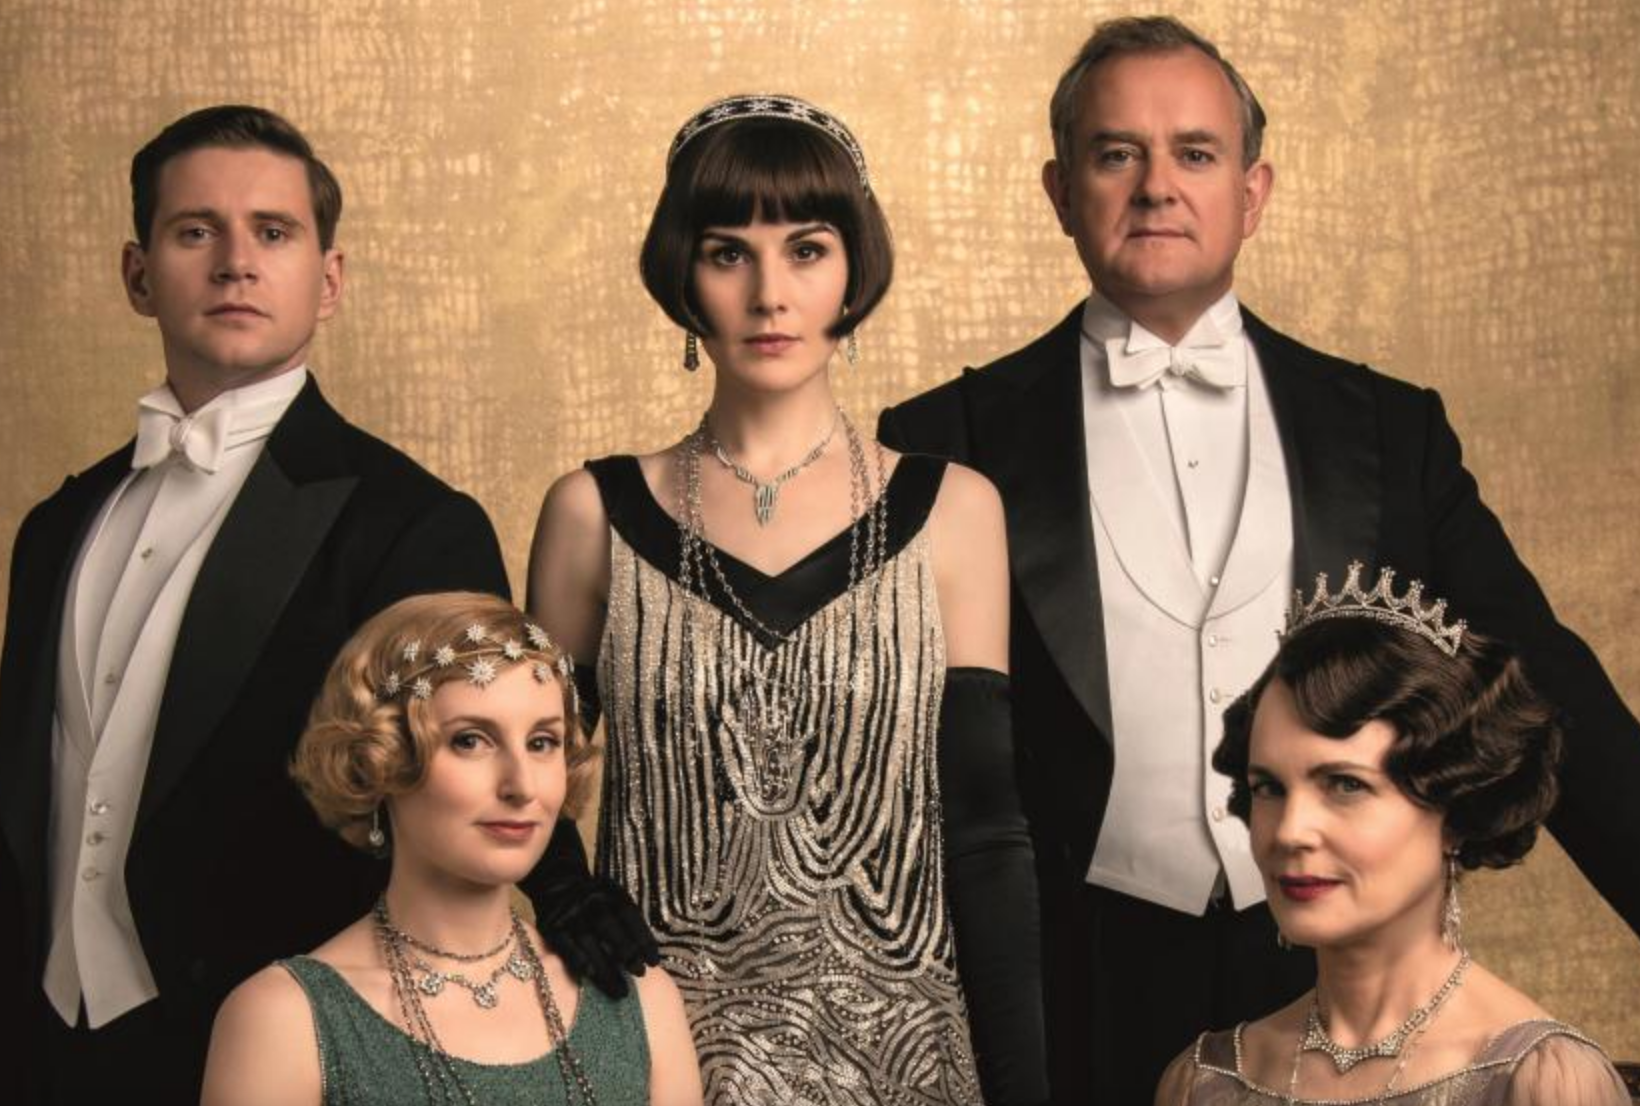
\includegraphics[scale=0.25]{downton.png}
\end{column}
\end{columns}

\end{frame}

%@@@@@@@@@@@@@@@@@@@@@@@@@@@@@@@@@@@@@@@@@@@@@@@@@
\begin{frame}
\frametitle{Stories of Change}
\begin{columns}
\begin{column}{0.5\textwidth}

\begin{itemize}
\item Two variations, \textbf{rising} and \textbf{declining}:
\begin{itemize}
\item Rising: things are becoming more favorable (e.g. post Communist Poland);
\item Declining: things are becoming less favorable (e.g. post WWI Britain);
\end{itemize}
\bigskip
\item Perhaps correlated with development:
\begin{itemize}
\item Developed countries' progress is past;
\item Developing countries current experience is material and technological progress;
\end{itemize}
\bigskip
\item `Change is only an illusion' -- (e.g. Why Most Published Research Findings Are False, Ioannidis 2005).
\end{itemize}

\end{column}
\begin{column}{0.5\textwidth}

\includegraphics[scale=0.15]{vanderbilt.jpg}
\end{column}
\end{columns}

\end{frame}

%@@@@@@@@@@@@@@@@@@@@@@@@@@@@@@@@@@@@@@@@@@@@@@@@@
\begin{frame}
\frametitle{Stories of Change}
\begin{columns}
\begin{column}{0.5\textwidth}

\begin{itemize}
\item Two variations, \textbf{rising} and \textbf{declining}:
\begin{itemize}
\item Rising: things are becoming more favorable (e.g. post Communist Poland);
\item Declining: things are becoming less favorable (e.g. post WWI Britain);
\end{itemize}
\bigskip
\item Perhaps correlated with development:
\begin{itemize}
\item Developed countries' progress is past;
\item Developing countries current experience is material and technological progress;
\end{itemize}
\bigskip
\item `Change is only an illusion' -- (e.g. Why Most Published Research Findings Are False, Ioannidis 2005).
\end{itemize}

\end{column}
\begin{column}{0.5\textwidth}
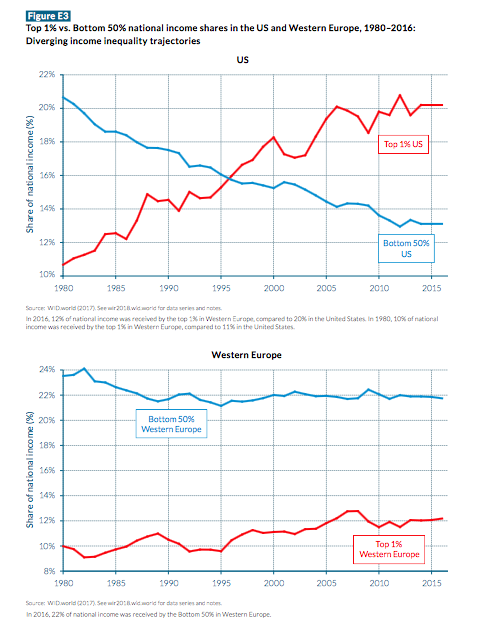
\includegraphics[scale=0.3]{inequality_US.png}
\end{column}
\end{columns}

\end{frame}

%@@@@@@@@@@@@@@@@@@@@@@@@@@@@@@@@@@@@@@@@@@@@@@@@@
\begin{frame}
\frametitle{Stories of Power}
\begin{itemize}
\item \textbf{Helplessness} and \textbf{Control}:
\begin{itemize}
\item ``This is bad but let me argue that this is a \textbf{problem} and not a \textbf{condition}";
\item Example: climate change;
\item Example: Keynesian economics;
\item Tied to Kingdon's streams metaphor;
\end{itemize}
\bigskip
\item Variations:
\begin{itemize}
\item Conspiracy: ``This is bad and under human control... but it's been controlled by a small group secretly who wants to harm you!"
\begin{itemize}
\item Shift issues from fate to human control;
\item Reveal harm has been deliberately caused or knowingly tolerated;
\item Call to wrest control from the few who benefit at the expense of the many;
\item e.g. the deep state, the financial crisis;
\end{itemize}
\bigskip
\item Blame-the-victim: ``This is bad but it's under \textbf{their} control so it's their fault!"
\begin{itemize}
\item Shift issues from fate to human control;
\item Locates control in the people who suffer from the problem;
\item End with a call for victims to reform their own behavior;
\item e.g. the financial crisis, students.
\end{itemize}
\end{itemize}
\end{itemize}
\end{frame}

%@@@@@@@@@@@@@@@@@@@@@@@@@@@@@@@@@@@@@@@@@@@@@@@@@
\begin{frame}
\frametitle{Stories of Power: blame the victim}
\begin{center}
During the State of the Union, President Obama called for a new era of responsibility, and declared that there will be ``no bailouts,” yet he offered a supposed solution for the ongoing mortgage crisis that rewards irresponsibility by promising even more bailouts for ``underwater” homeowners.\\
\bigskip
From \href{https://www.nytimes.com/roomfordebate/2012/01/25/is-refinancing-the-best-way-to-fix-the-housing-market/mortgage-crisis-stop-rewarding-irresponsible-consumers}{Mortgage Crisis: Stop Rewarding Irresponsible Consumers}
\end{center}
\end{frame}

%@@@@@@@@@@@@@@@@@@@@@@@@@@@@@@@@@@@@@@@@@@@@@@@@@
\begin{frame}
\frametitle{Narrative Types}
\begin{itemize}
\item Synecdoche: the whole represented by one of its parts:
\begin{itemize}
\item OSHA tooth regulation;
\item Ticking time bomb terrorist;
\item Stone's presentation of the market model;
\end{itemize}
\bigskip
\bigskip
\item Metaphor: if $A$ is like $B$ then we can solve $A$ the way we've solved $B$:
\begin{itemize}
\item Organisms (organizations have goals);
\item Natural laws (Malthus); 
\item Machines (economics);
\item Wedges/Slippery slopes/Scale changes (gun control);
\item Containers (borders, power vacuum);
\item Disease (communism);
\item War (drugs, COVID).
\end{itemize}
\end{itemize}
\end{frame}

%%@@@@@@@@@@@@@@@@@@@@@@@@@@@@@@@@@@@@@@@@@@@@@@@@@
%\begin{frame}
%\frametitle{Ambiguity}
%\begin{itemize}
%\item Symbols are \textbf{ambiguous} -- they can mean more than one thing simultaneously;
%\bigskip
%\bigskip
%\item Facilitates negotiation and cooperation (e.g. unite people who want different policies);
%\bigskip
%\bigskip
%\item Enables getting things done (or appearing to, e.g. derivative regulation);
%\bigskip
%\bigskip
%\item Allows for expression of two sentiments simultaneously (e.g. apology to Native Peoples).
%\end{itemize}
%\end{frame}

%@@@@@@@@@@@@@@@@@@@@@@@@@@@@@@@@@@@@@@@@@@@@@@@@@
\begin{frame}

\begin{center}
\Huge\textbf{Why should we care?}\\
\bigskip
\bigskip
\large Political actors use symbols that define problems in ways that will persuade doubters and attract support\\
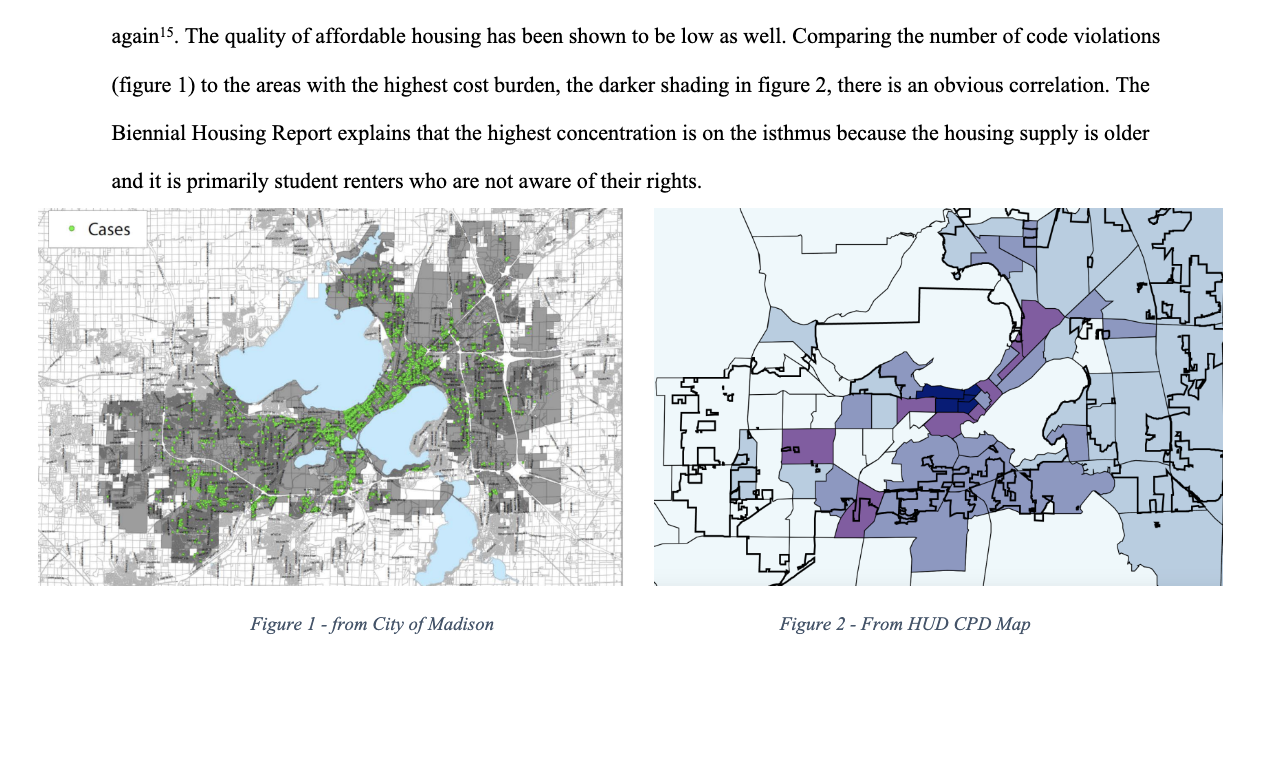
\includegraphics[scale=0.2]{maps.png}
\end{center}

\end{frame}



%@@@@@@@@@@@@@@@@@@@@@@@@@@@@@@@@@@@@@@@@@@@@@@@@@
\begin{frame}

\begin{center}
\Huge\textbf{Problems : Numbers}\\
\bigskip
\bigskip
\large Describing with numbers
\end{center}

\end{frame}

%%@@@@@@@@@@@@@@@@@@@@@@@@@@@@@@@@@@@@@@@@@@@@@@@@@
%\begin{frame}
%\frametitle{Choices}
%\begin{itemize}
%\item How do we measure unemployment?
%\begin{itemize}
%\item \textbf{Decide} what the measure is supposed to capture: need for jobs;
%\item \textbf{Transform} this into something observable: people wanting work;
%\item \textbf{Operationalize} by fixing inclusion criteria: older than 16, had a job previously, have looked in previous 4 weeks, and are available;
%\end{itemize}
%\bigskip
%\bigskip
%\item Definition of measurement $=$ definition of the problem and therefore a main avenue of political conflict;
%\bigskip
%\bigskip
%\item Stone wonders about those who...
%\begin{itemize}
%\item ...can get dangerous/demeaning/unpleasant jobs but don't;
%\item ...could get part time but hold out for full time;
%\item ...quit to find something better but are still searching;
%\item ...can get a job but can't find child care to take a job;
%\item ...have never worked but want to now.
%\end{itemize}
%
%\end{itemize}
%\end{frame}


%@@@@@@@@@@@@@@@@@@@@@@@@@@@@@@@@@@@@@@@@@@@@@@@@@
\begin{frame}
\frametitle{Choices}
\begin{center}
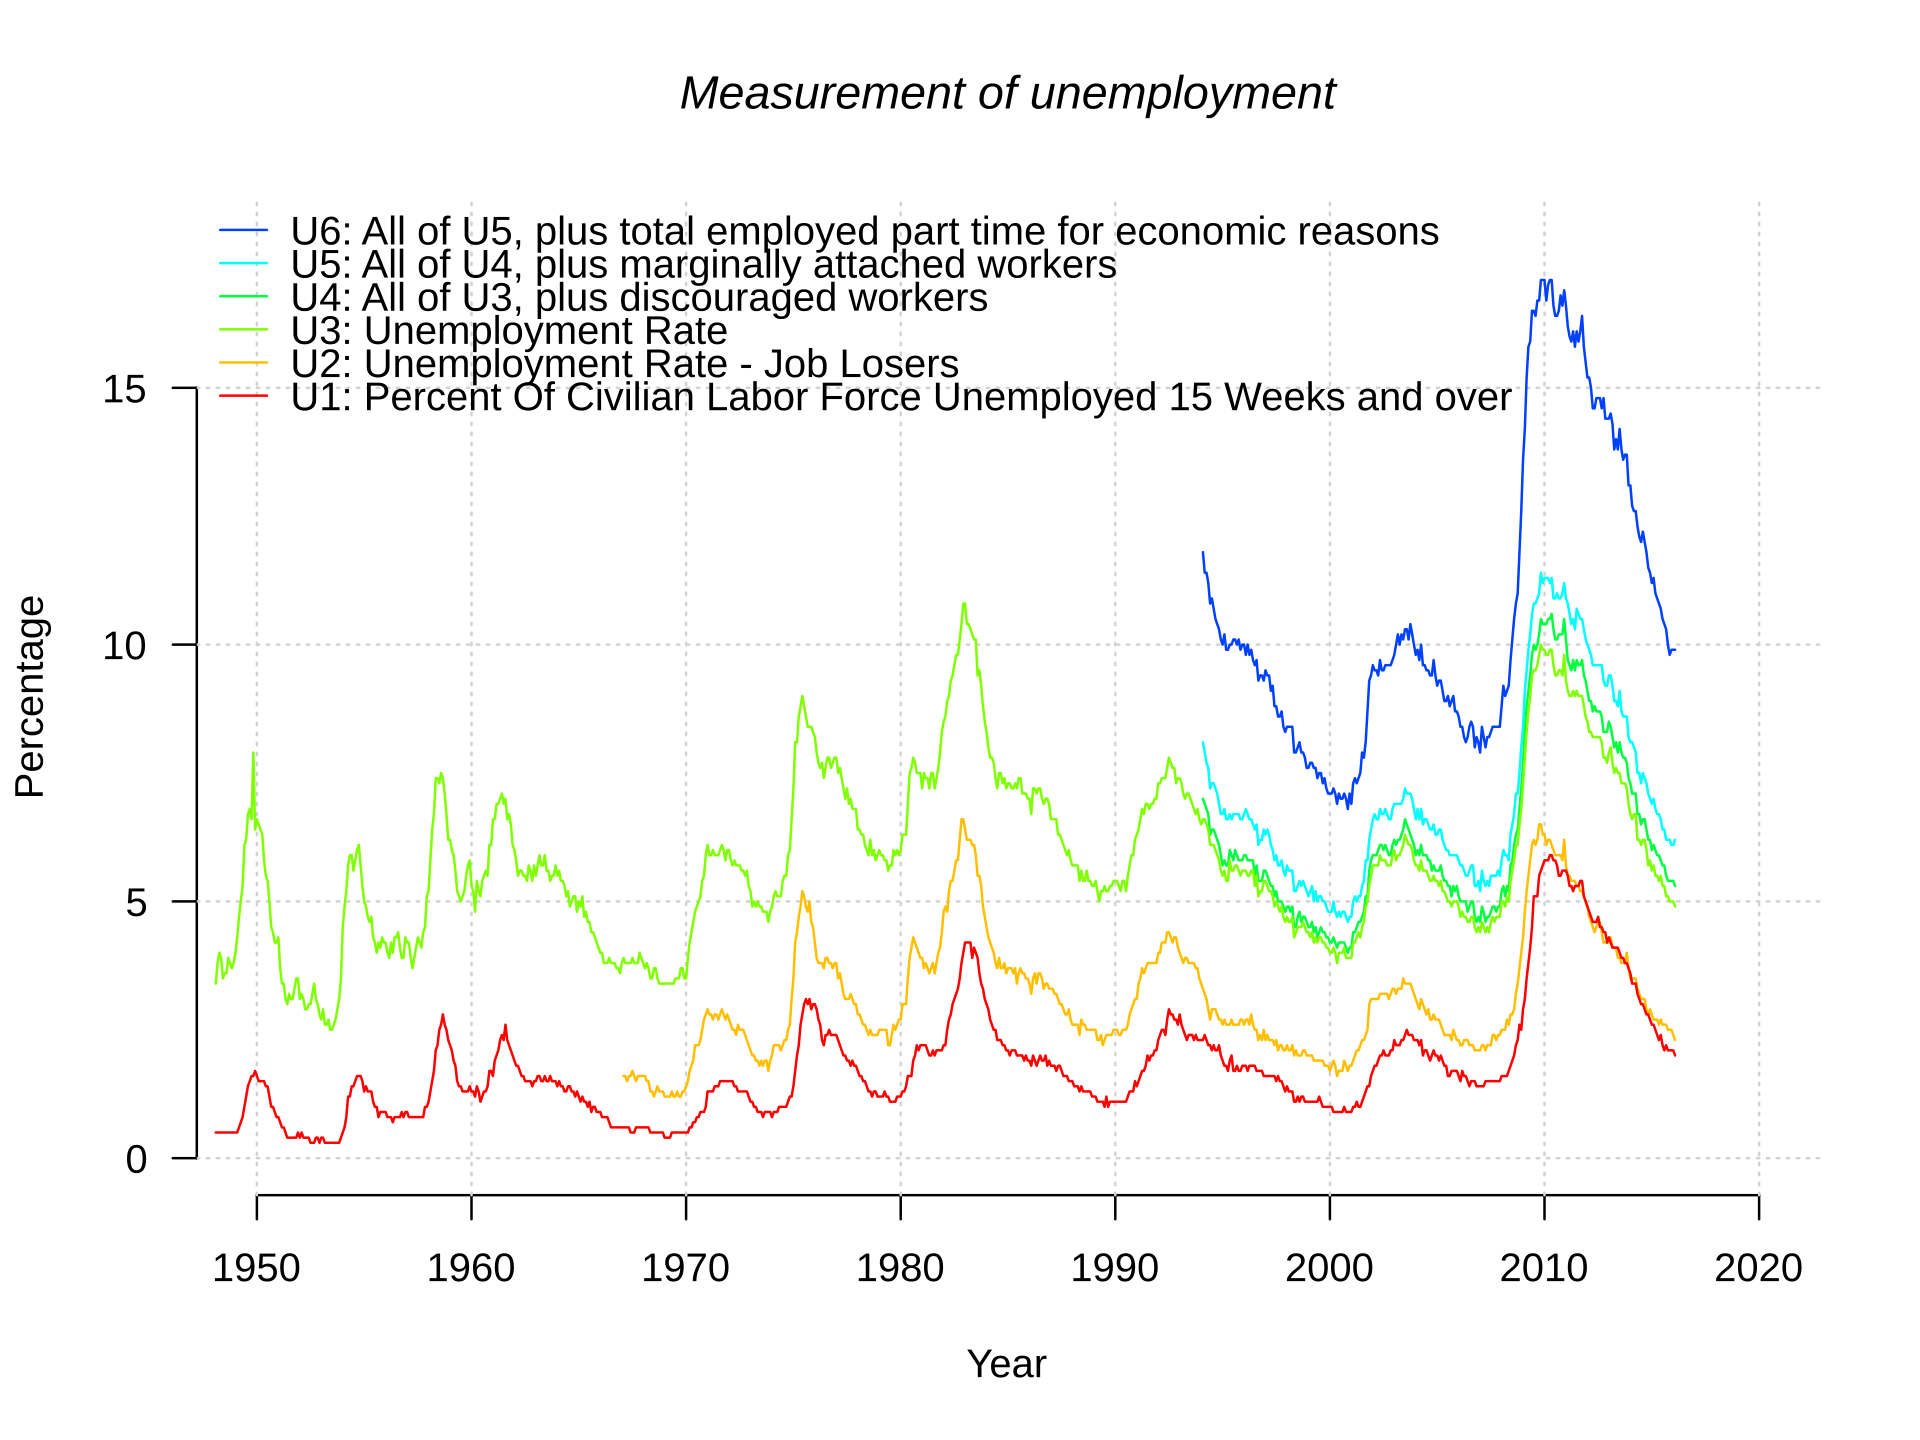
\includegraphics[scale=0.15]{unemployment_2.png}
\end{center}

\end{frame}

%@@@@@@@@@@@@@@@@@@@@@@@@@@@@@@@@@@@@@@@@@@@@@@@@@
\begin{frame}
\frametitle{Choices}

\begin{itemize}
\item How many public water systems are there in the US?
\bigskip
\bigskip
\item Public water system: $\geq$15 service connections or service to an average of $\geq$ 25 people for $\geq$ 60 days a year;
\bigskip
\bigskip
\item With this definition, over 148k;
\begin{itemize}
\item Community Water System;
\item Non-Transient Non-Community Water System;
\item Transient Non-Community Water System.
\end{itemize}
\end{itemize}

\end{frame}



%@@@@@@@@@@@@@@@@@@@@@@@@@@@@@@@@@@@@@@@@@@@@@@@@@
\begin{frame}
\frametitle{Choices}
\begin{itemize}
\item ``As answers to policy problems, the resolution numbers offer is nothing more than a human decision about how to count as"  (i.e. numbers $=$ metaphors);
\bigskip
\bigskip
\item Wrongful exclusion:
\begin{itemize}
\item Assertion of a likeness where measurement assigns a difference;
\item Examples: unemployed, homelessness, grades, excess mortality during war;
\end{itemize}
\bigskip
\bigskip
\item Wrongful inclusion:
\begin{itemize}
\item Assertion of a difference where measurement assigns a likeness;
\item Example: excess mortality during war (Iraq war deaths);
\end{itemize}
\end{itemize}
\end{frame}

%%@@@@@@@@@@@@@@@@@@@@@@@@@@@@@@@@@@@@@@@@@@@@@@@@@
%\begin{frame}
%\frametitle{Hidden messages in using numbers}
%\begin{itemize}
%\item Expertise and authority (e.g. Mitt Romney);
%\bigskip
%\bigskip
%\item Recognition or assertion that something is widespread but unobserved (e.g. COVID);
%\bigskip
%\bigskip
%\item Claim of clear boundaries (e.g. insurgency);
%\bigskip
%\bigskip
%\item Creation of community (e.g. population);
%\bigskip
%\bigskip
%\item Bargaining (e.g. breaking down a problem like Roe v Wade).
%\end{itemize}
%\end{frame}

%@@@@@@@@@@@@@@@@@@@@@@@@@@@@@@@@@@@@@@@@@@@@@@@@@
\begin{frame}
\frametitle{Artifacts and dangers...}
\begin{columns}
\begin{column}{0.5\textwidth}

\begin{itemize}
\item Numbers can reduce conflicts to a single dimension;
\begin{itemize}
\item e.g., if we only considered the energy density of fuel sources (versus cost or safety), we might draft policy to build more nuclear power plants...
\end{itemize} 
\item Numbers legitimize political decisions;
\begin{itemize}
\item ...and sometimes mask the political nature of a decision;
\item For example, numbers suggest that safety can be defined though science (but recall the complexity and subjective nature of ``Security");
\item Back to Egan: What is a ``safe number of organisms that could be discharged per cubic meter of water?"
\end{itemize}
\end{itemize}

\end{column}
\begin{column}{0.5\textwidth}
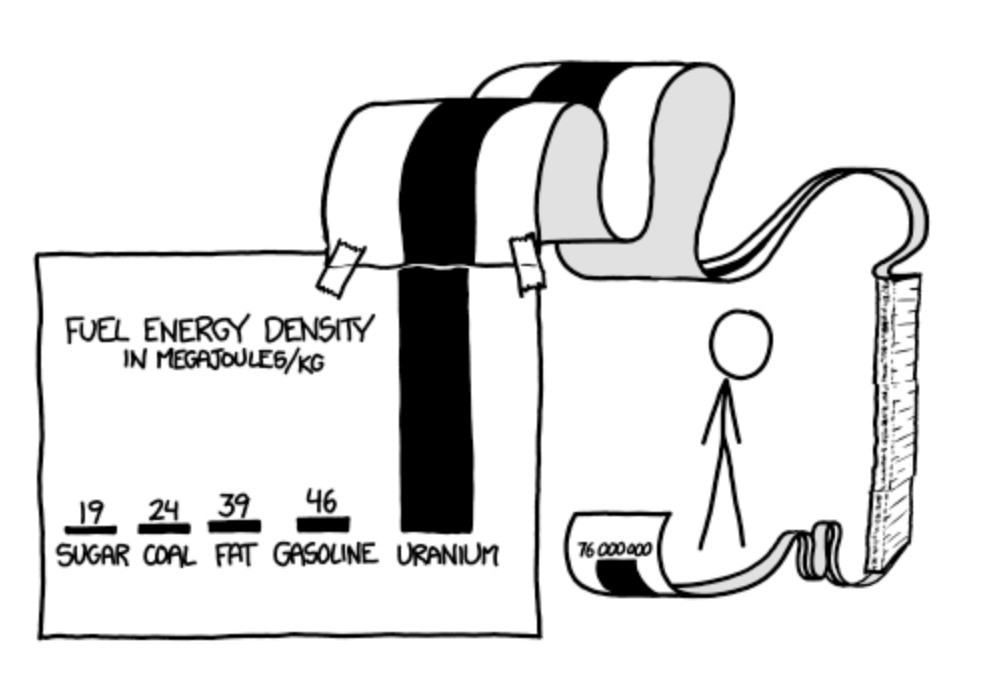
\includegraphics[scale=0.4]{energy.png}
\end{column}
\end{columns}

\end{frame}

%@@@@@@@@@@@@@@@@@@@@@@@@@@@@@@@@@@@@@@@@@@@@@@@@@
\begin{frame}
\frametitle{Artifacts and dangers...}
\begin{columns}
\begin{column}{0.5\textwidth}

\begin{itemize}
\item Numbers can reduce conflicts to a single dimension;
\begin{itemize}
\item e.g., if we only considered the energy density of fuel sources (versus cost or safety), we might draft policy to build more nuclear power plants...
\end{itemize}
\item Numbers legitimize political decisions;
\begin{itemize}
\item ...and sometimes mask the political nature of a decision;
\item For example, numbers suggest that safety can be defined though science (but recall the complexity and subjective nature of ``Security");
\item Back to Egan: What is a ``safe number of organisms that could be discharged per cubic meter of water?"
\end{itemize}
\end{itemize}

\end{column}
\begin{column}{0.5\textwidth}
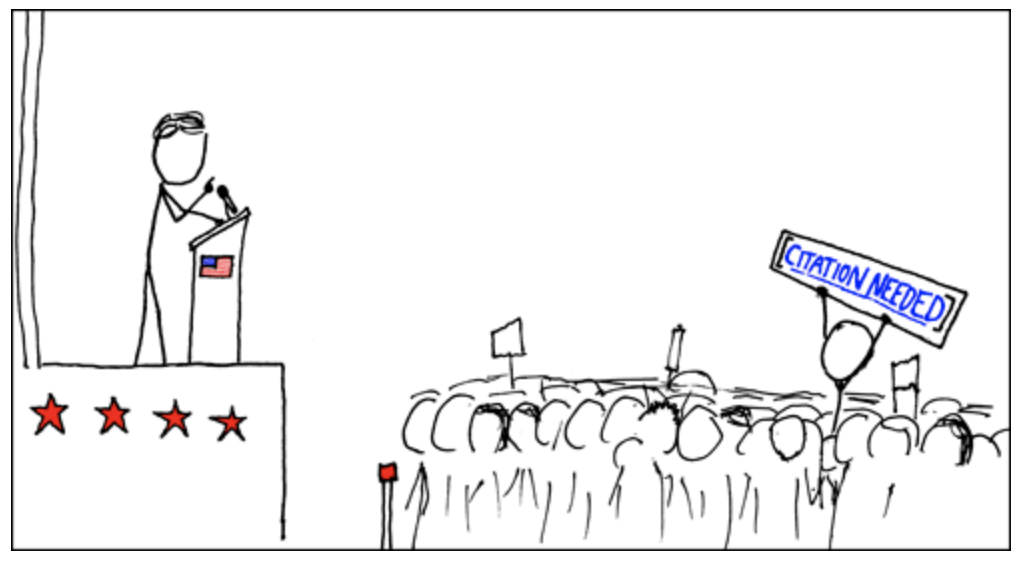
\includegraphics[scale=0.4]{speech.png}
\end{column}
\end{columns}

\end{frame}

%@@@@@@@@@@@@@@@@@@@@@@@@@@@@@@@@@@@@@@@@@@@@@@@@@
\begin{frame}
\frametitle{Observer Effects}
\begin{itemize}
\item In science (especially social science), we confront observer effects–the fact that things, and especially people, behave differently when observed;
\begin{itemize}
\item Physics: uncertainty (Heisenberg) and it's generalizations;
\item Social science: poll responses;
\end{itemize}
\bigskip
\item Can interact with counting -- by counting people as part of a group, a policy may induce them to act as a group (statistical community becomes a natural community). Group theories of politics (e.g., pluralism) tell us to expect these groups to then advocate for resources, privileges, or protection in future policy processes.
\bigskip
\item Question: if the Department of Justice Antitrust Division measures market concentration to decide whether to permit corporate mergers and acquisitions, how do you think this might affect how large companies lobby regarding the definition of their ``market"?
\end{itemize}
\end{frame}

%@@@@@@@@@@@@@@@@@@@@@@@@@@@@@@@@@@@@@@@@@@@@@@@@@
\begin{frame}

\begin{center}
\Huge\textbf{Why should we care?}\\
\bigskip
\bigskip
\large The power to measure is the power to control.  Measurers have a lot of discretion in their choice of what and how to measure.\\
\end{center}

\end{frame}

%@@@@@@@@@@@@@@@@@@@@@@@@@@@@@@@@@@@@@@@@@@@@@@@@@
\begin{frame}

\begin{center}
\Huge\textbf{Problems : Causes}\\
\bigskip
\bigskip
\large How the world works
\end{center}

\end{frame}

%@@@@@@@@@@@@@@@@@@@@@@@@@@@@@@@@@@@@@@@@@@@@@@@@@
\begin{frame}
\frametitle{To Know the Causes of Things}
\begin{itemize}
\item \textbf{Causality}: necessary and sufficient conditions;
\begin{itemize}
\item Very difficult;
\item Absolutely crucial for effective problem solving;
\end{itemize}
\bigskip
\bigskip
\item Ideal: causes are objective and can be identified by scientific analysis;
\bigskip
\bigskip
\item Stone: causal analysis has prescriptive power:
\begin{itemize}
\item Like numbers, causes highlight some aspects of a problem and ignore others;
\item Causal chains are stories that define problems and assign blame;
\item Because they have this power there are incentives to use them strategically.
\end{itemize}
\end{itemize}
\end{frame}

%@@@@@@@@@@@@@@@@@@@@@@@@@@@@@@@@@@@@@@@@@@@@@@@@@
\begin{frame}
\frametitle{Typology of causal theories (Table 9.1)}
\begin{itemize}
\item Unguided actions/Intended consequences -- \textbf{mechanical cause}:
\begin{itemize}
\item Machines that perform to spec but cause harm;
\item Rigid bureaucratic routines;
\end{itemize}
\bigskip
\item Unguided actions/unintended consequences -- \textbf{accidental cause}:
\begin{itemize}
\item Natural disasters;
\item Fate/bad luck;
\end{itemize}
\bigskip
\item Guided actions/Intended consequences -- \textbf{intentional cause}:
\begin{itemize}
\item Oppression;
\item Conspiracy;
\item Known but ignored harms;
\item Victim blaming;
\end{itemize}
\bigskip
\item Guided actions/unintended consequences -- \textbf{inadvertent cause}:
\begin{itemize}
\item unintended side effects;
\item Victim blaming.
\end{itemize}
\end{itemize}
\end{frame}

%@@@@@@@@@@@@@@@@@@@@@@@@@@@@@@@@@@@@@@@@@@@@@@@@@
\begin{frame}
\frametitle{Complexity}
\begin{itemize}
\item Many policy problems--such as toxic hazards, global warming, oil spills, and food safety--require a more \textbf{complex model of cause}... can shift problems to appear accidental or unintended;
\bigskip
\item Complex systems:
\begin{itemize}
\item Social systems necessary to solve modern problems are inherently complex;
\item Multiple actors $+$ complex feedback loops $=$ certain but impossible to anticipate failure;
\end{itemize}
\bigskip
\item Institutional complexity:
\begin{itemize}
\item Social problems caused by webs of large organizations with built-in incentive structures and patterns of behavior;
\item e.g. US government procurement;
\end{itemize}
\bigskip
\item Historical complexity:
\begin{itemize}
\item Decisions in one period determine the choices available in future periods;
\item Path dependence -- e.g. QWERTY keyboards.
\end{itemize}
\end{itemize}
\end{frame}

%%@@@@@@@@@@@@@@@@@@@@@@@@@@@@@@@@@@@@@@@@@@@@@@@@@
%\begin{frame}
%\frametitle{The banality of evil}
%\begin{itemize}
%\item These questions of intentionality and complexity are essential to the concept of accountability;
%\bigskip
%\bigskip
%\item ``I was just following orders" $\sim$ Adolf Eichmann;
%\begin{itemize}
%\item If Eichmann’s work, as a bureaucrat, is seen as a mechanical process of following orders or as embedded in a complex system, then he is not a policy actor and thus not responsible;
%\item If seen as an intentional architect, then he is a policy actor and thus entirely responsible;
%\end{itemize}
%\bigskip
%\bigskip
%\item Not just for the Holocaust -- the podcast, Death by a Thousand Cuts applied philosopher Hannah Arendt’s concept of “the Banality of Evil” to agency decisions;
%\bigskip
%\bigskip
%\item How might we draw lines between people who are simply following orders and thus blameless and those who act consciously, and are thus responsible?
%\end{itemize}
%\end{frame}

%%@@@@@@@@@@@@@@@@@@@@@@@@@@@@@@@@@@@@@@@@@@@@@@@@@
%\begin{frame}
%\frametitle{Legitimacy}
%\begin{itemize}
%\item Science: arbiter of empirical questions;
%\bigskip
%\bigskip
%\item Law: hears claims, examines evidence, pronounces judgments;
%\bigskip
%\bigskip
%\item This is why good research and understanding of legal authority are so important for writing policy memos. Without evidence and authority that your audience sees as legitimate, they will not take your recommendations seriously.
%\end{itemize}
%\end{frame}

%@@@@@@@@@@@@@@@@@@@@@@@@@@@@@@@@@@@@@@@@@@@@@@@@@
\begin{frame}

\begin{center}
\Huge\textbf{Why should we care?}\\
\bigskip
\bigskip
\large The role of causality is why good research and understanding of legal authority are so important for writing policy memos. Without evidence and authority that your audience sees as legitimate, they will not take your recommendations seriously.\\
\bigskip
Causal theories are efforts to control interpretations and images of problems, to describe harms and difficulties, to attribute them to actions of actors, and thereby to allocate government power to stop the harm.
\\
\end{center}

\end{frame}

%@@@@@@@@@@@@@@@@@@@@@@@@@@@@@@@@@@@@@@@@@@@@@@@@@
\begin{frame}

\begin{center}
\Huge\textbf{Problems : Interests}\\
\bigskip
\bigskip
\large Who is affected and in what way
\end{center}

\end{frame}

%@@@@@@@@@@@@@@@@@@@@@@@@@@@@@@@@@@@@@@@@@@@@@@@@@
\begin{frame}
\frametitle{How are interests represented?}
\begin{itemize}
\item In the market model of society: 
\begin{itemize}
\item Actors know their own tastes/preferences better than anybody else (perfect info?);
\item Leaders don't need to define other people's interests;
\item Actor goal is to maximize utility;
\end{itemize}
\bigskip
\bigskip
\item In the polis model of society:
\begin{itemize}
\item Actors don't enter politics with well-defined interests;
\item Leaders try to gather support for proposed policies by explaining to actors what their interests are;
\item Group identities and memberships shape actor interests;
\end{itemize}
\bigskip
\bigskip
\item Example -- black woman who is a small business owner and parent:
\begin{itemize}
\item Black (race, NAACP);
\item Woman (gender, NOW);
\item Small business owner (class, Chamber of Commerce);
\item Parent (family status, MADD).
\end{itemize}
\end{itemize}
\end{frame}

%@@@@@@@@@@@@@@@@@@@@@@@@@@@@@@@@@@@@@@@@@@@@@@@@@
\begin{frame}
\frametitle{Mobilizing Interests}
\begin{itemize}
\item \textbf{Mobilization}: when people understand their problems are shared by others and they organize to influence policy;
\item How does it happen?
\begin{itemize}
\item Pluralism -- if people are adversely affected by a social condition they will organize;
\item Rational choice -- group formation will be rare b/c \textbf{prisoner's dilemma} and \textbf{free riding};
\end{itemize}
\item Prisoner's dilemma (nobody uses this anymore!):
\begin{table}[]
\begin{tabular}{cccc}
 &  & Actor 2 & \\
 &&Confess& Clam up\\
  & Confess & \textbf{-5},\textbf{-5} & \textbf{0},-10\\
Actor 1 & Clam up & -10,\textbf{0}&-1,-1
\end{tabular}
\end{table}
Problem here isn't that actors can't talk - it's that they can't make post-game enforceable contracts (but see repeated PD);
\item Free riding: public goods mean that everybody receives benefits even with no work (but see The Logic of Collective Action Olson 1965).
\end{itemize}
\end{frame}

%@@@@@@@@@@@@@@@@@@@@@@@@@@@@@@@@@@@@@@@@@@@@@@@@@
\begin{frame}
\frametitle{Mobilizing Interests}
\begin{itemize}
\item Stone: groups do form (thus falsifying rational choice) but don't get equal opportunity to influence policy (thus falsifying pluralism);
\begin{itemize}
\item Note: Stone is conflating rational choice w/ prisoner's dilemma (i.e. a synecdoche) -- this is not correct, e.g. coop. game theory, non-coop. game theory w/ self-enforcing coalitions;
\end{itemize}
\bigskip
\bigskip
\item In the polis:
\begin{itemize}
\item Actors have \textbf{ties} (e.g. parents, friends, partners, teachers, bosses, and cultural heroes); 
\item Ties create strong \textbf{mechanisms} of influence and moral leadership;
\item Mechanisms create \textbf{norms} (e.g. altruism, reciprocity, cooperation) and ready channels for collective action;
\item All of these factors create \textbf{social capital}, which, like physical assets or material wealth, can be used to harness individual energies for the common good;
\end{itemize}
\end{itemize}
%\begin{quote}
%\small Collective action in politics is more like a sports competition than a bargain hunt. One plays to win, and winning gives the game its direction and structure, but one place even more just to play, and the greater satisfaction comes from being in the game. Seen in this light, the costs of collective action such as the time and effort are its benefits.  (Stone, p 237)
%\end{quote}
\end{frame}

%@@@@@@@@@@@@@@@@@@@@@@@@@@@@@@@@@@@@@@@@@@@@@@@@@
\begin{frame}
\frametitle{Issues and interests define each other}
\begin{itemize}
\item Different policy tools generate different kinds of politics:
\begin{table}[]
\begin{tabular}{lll}
&Concentrated Benefits&Diffuse Benefits\\
Concentrated Costs&\textbf{Interest Group Politics}&\textbf{Entrepeneurial Politics}\\
&Social security&Tariffs\\
&Sales tax&State mandated health insurance\\
&Stalemate/alternating victory&Status Quo\\
Diffuse Costs&\textbf{Clientele politics} & \textbf{Majoritarian politics}\\
&Food safety regulation&Labor-management bargaining\\
&Carbon tax&\\
&Rapid change&Gradual expansion
\end{tabular}
\end{table}
\bigskip
\bigskip
\item Stone: ``Programs don’t themselves have inherent distributions of costs and benefits. Rather, political actors strategically represent programs as contests between different types of costs and benefits."
\end{itemize}
\end{frame}

%@@@@@@@@@@@@@@@@@@@@@@@@@@@@@@@@@@@@@@@@@@@@@@@@@
\begin{frame}

\begin{center}
\Huge\textbf{Why should we care?}\\
\bigskip
\bigskip
\large An effective policy memo analyzes the political terrain of existing stakeholder groups and anticipates how stakeholder interests that might be mobilized by policy, even interest groups that are not yet mobilized or do not yet exist because policy proposals create interests.
\\
\end{center}

\end{frame}

%@@@@@@@@@@@@@@@@@@@@@@@@@@@@@@@@@@@@@@@@@@@@@@@@@
\begin{frame}

\begin{center}
\Huge\textbf{Problems : Decisions}\\
\bigskip
\bigskip
\large Optimization?
\end{center}

\end{frame}

%@@@@@@@@@@@@@@@@@@@@@@@@@@@@@@@@@@@@@@@@@@@@@@@@@
\begin{frame}
\frametitle{How do we choose?}
\begin{itemize}
\item \textbf{Rational choice (used by policy makers internally?)} -- a policy problem is a choice facing a political actor:
\begin{itemize}
\item Given a fixed goal...
\item Given an enumerated list of alternative means for attaining the goal...
\item Estimate consequences for each alternative;
\item Choose the alternative most likely to attain the goal;
\end{itemize}
\bigskip
\item Most rational choice approaches connect the second two with optimization;
\bigskip
\item \textbf{Polis (clearly external)}:
\begin{itemize}
\item Define goals ambiguously to maximize support (e.g. Greenspan);
\item Keep undesirable alternatives off the agenda by not mentioning them;
\item Make your preferred alternative appear to be the only feasible or possible one;
\item Focus on one part of the causal chain and ignore others that would require politically difficult or costly policy actions;
\item Blend alternatives to avoid triggering opposition;
\item Select only consequences whose costs and benefits will make your preferred course of action look best.
\end{itemize}
\bigskip
\item
\end{itemize}
\end{frame}

%@@@@@@@@@@@@@@@@@@@@@@@@@@@@@@@@@@@@@@@@@@@@@@@@@
\begin{frame}
\frametitle{Control over decisions}
\begin{itemize}
\item \textbf{Issue framing}: the process of focusing attention on a particular slice of an extended causal chain;
\bigskip
\item Recall the COVID vaccine example:
\begin{itemize}
\item Same expected values;
\item Changing labels (``lives saved" vs. ``deaths") can turn most people from risk-tolerant to risk-averse $=$ power of issue framing;
\end{itemize}
\bigskip
\item Suggests that choices among policy options depend on more than their expected outcomes;
\bigskip
\item \textbf{Hobson's Choice}: an either/or choice in which one choice is clearly terrible:
\begin{itemize}
\item e.g. Friedman's ``central direction involving the use of coercion" vs ``voluntary cooperation";
\item It's a trap!  Disarm it by imagining more possibilities;
\end{itemize}
\end{itemize}
\end{frame}

%%@@@@@@@@@@@@@@@@@@@@@@@@@@@@@@@@@@@@@@@@@@@@@@@@@
%\begin{frame}
%\frametitle{Cost-Benefit Analysis}
%\begin{itemize}
%\item \textbf{Cost-Benefit analysis}: comparing alternatives via listing pros and cons (often costed in dollars);
%\bigskip
%\bigskip
%\item Some concerns:
%\begin{itemize}
%\item Implies there are as many measurement problems as there are pros and cons;
%\item Consequences of an action are often intangibles and hard to define - very hard;
%\item Can lead to taking potential choice variables as fixed constraints (e.g. prices);
%\item Can lead analysts to ignore stuff that can't be costed (e.g. urban decline, damage reputations, loss of wilderness, loss of psychological insecurity);
%\item Can be strategically manipulated;
%\end{itemize}
%\bigskip
%\bigskip
%\item Stone: instead of taking prices as fixed, analyze the forces that create prices and make efforts to changing prices by changing the power relations that set them.
%\end{itemize}
%\end{frame}

%@@@@@@@@@@@@@@@@@@@@@@@@@@@@@@@@@@@@@@@@@@@@@@@@@
\begin{frame}
\frametitle{Utilitarian vs. deontological decision-making}
\begin{itemize}
\item \textbf{Utilitarianism (normative ethical theory)}: the morality of an action should be based on consequences, specifically maximizing the resulting good or utility;
\bigskip
\bigskip
\item \textbf{Deontology (also normative ethical theory)}: the morality of an action should be based on whether that action itself is right or wrong under a series of rules;
\bigskip
\bigskip
\item What are the arguments for/against torture?
\bigskip
\bigskip
\item Is the Constitution utilitarian or deontological?
\end{itemize}
\end{frame}

%@@@@@@@@@@@@@@@@@@@@@@@@@@@@@@@@@@@@@@@@@@@@@@@@@
\begin{frame}
\frametitle{Utilitarian vs. deontological decision-making}
\begin{columns}
\begin{column}{0.5\textwidth}

``Converting the Great Lakes fishery from one that was essentially managed as a self-sustaining public food supply into one that was intensively managed for the thrill of recreational anglers was, for Tanner, a natural evolution.  ``\textbf{You manage the resource to produce the greatest good for the greatest number for the longest period of time}," Tanner said, borrowing the axiom of the first boss of the U.S. Forest Service, Gifford Pinchot." -- Egan, p. 84.

\end{column}
\begin{column}{0.5\textwidth}
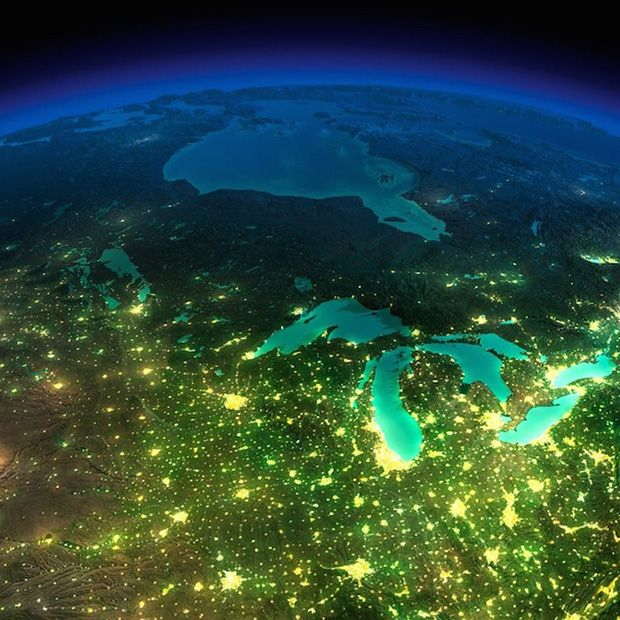
\includegraphics[scale=0.3]{great_lakes.jpg}
\end{column}
\end{columns}


\end{frame}

%@@@@@@@@@@@@@@@@@@@@@@@@@@@@@@@@@@@@@@@@@@@@@@@@@
\begin{frame}

\begin{center}
\Huge\textbf{Why should we care?}\\
\bigskip
\bigskip
\large This is why it is important to compare good options–that is, options your reader will agree are some of the best things they might do. If the options you present appear to bias the decision, they are not going to take your analysis seriously. But, of course, the options you choose will always affect the decision! The trick is to present options that don’t make your analysis seem pre-judged or tilted to a particular outcome.
\\
\end{center}

\end{frame}

%@@@@@@@@@@@@@@@@@@@@@@@@@@@@@@@@@@@@@@@@@@@@@@@@@
\begin{frame}
\frametitle{Birkland$+$ Model of Policy}
\begin{itemize}
\item Policy Domain: what substantive problems are under consideration?  This specifies:
\begin{itemize}
\item The actors involved, official actors who can make decisions $+$ stakeholders; 
\item Distribution of benefits/costs $\Rightarrow$ actor organization, e.g. iron triangle, policy community;
\item The systemic agenda; 
\end{itemize}
\bigskip
\item \color{black}Input-output Model;
\begin{itemize}
\item Actors: legislature, executive, bureaucrats, justices and the available levers;
\item Inputs: agenda setting (application of power/social construction, focusing events, indicator change driven esp by unofficial actors) sets goals, determines the causal model, which specifies the institutional agenda, and leads to the policies on the decision agenda;
\item Black box decision making, timing (incrementalism, punctuated eq) driven by indicators/focusing events, choice driven by e.g. median voter thm, Arrow's thm;
\begin{itemize}
\item Round 1: works on decision agenda, leads to outputs (e.g. statute laws, rules, court decisions);
\item Round 2: Implementation, leads to outcomes;
 \end{itemize}
\end{itemize}
\bigskip
\item Outcomes: Feedback from failure and success, learning leads to iteration and updates.
\end{itemize}
\end{frame}

%@@@@@@@@@@@@@@@@@@@@@@@@@@@@@@@@@@@@@@@@@@@@@@@@@
\begin{frame}
\frametitle{Birkland$+$ Model of Policy, goals}
\begin{itemize}
\item Policy Domain: what substantive problems are under consideration?  This specifies:
\begin{itemize}
\item The actors involved, official actors who can make decisions $+$ stakeholders; 
\item Distribution of benefits/costs $\Rightarrow$ actor organization, e.g. iron triangle, policy community;
\item The systemic agenda; 
\end{itemize}
\bigskip
\item \color{black}Input-output Model;
\begin{itemize}
\item Actors: legislature, executive, bureaucrats, justices and the available levers;
\item Inputs: agenda setting (application of power/social construction, focusing events, indicator change driven esp by unofficial actors) \textbf{sets goals}, determines the causal model, which specifies the institutional agenda, and leads to the policies on the decision agenda;
\item Black box decision making, timing (incrementalism, punctuated eq) driven by indicators/focusing events, choice driven by e.g. median voter thm, Arrow's thm;
\begin{itemize}
\item Round 1: works on decision agenda, leads to outputs (e.g. statute laws, rules, court decisions);
\item Round 2: Implementation, leads to outcomes;
 \end{itemize}
\end{itemize}
\bigskip
\item Outcomes: Feedback from failure and success, learning leads to iteration and updates.
\end{itemize}
\end{frame}

%@@@@@@@@@@@@@@@@@@@@@@@@@@@@@@@@@@@@@@@@@@@@@@@@@
\begin{frame}
\frametitle{Birkland$+$ Model of Policy, goals, problems}
\begin{itemize}
\item Policy Domain: what substantive problems are under consideration?  This specifies:
\begin{itemize}
\item The actors involved, official actors who can make decisions $+$ \textbf{stakeholders}; 
\item \textbf{Distribution of benefits/costs} $\Rightarrow$ actor organization, e.g. iron triangle, policy community;
\item The systemic agenda; 
\end{itemize}
\bigskip
\item \color{black}Input-output Model;
\begin{itemize}
\item Actors: legislature, executive, bureaucrats, justices and the available levers;
\item Inputs: \textbf{agenda setting (application of power/social construction, focusing events, indicator change driven esp by unofficial actors)} \textbf{sets goals}, \textbf{determines the causal model}, which specifies the institutional agenda, and leads to the policies on the decision agenda;
\item Black box \textbf{decision making, timing (incrementalism, punctuated eq) driven by indicators/focusing events}, choice driven by e.g. median voter thm, Arrow's thm;
\begin{itemize}
\item Round 1: works on decision agenda, leads to outputs (e.g. statute laws, rules, court decisions);
\item Round 2: Implementation, leads to outcomes;
 \end{itemize}
\end{itemize}
\bigskip
\item Outcomes: \textbf{Feedback from failure and success}, learning leads to iteration and updates.
\end{itemize}
\end{frame}
%symbols, numbers, causes, interests, decisions

%@@@@@@@@@@@@@@@@@@@@@@@@@@@@@@@@@@@@@@@@@@@@@@@@@
\begin{frame}

\begin{center}
\Huge\textbf{Solutions : Incentives}\\
\bigskip
\bigskip
\large Behavior change through rewards and penalties
\end{center}

\end{frame}

%@@@@@@@@@@@@@@@@@@@@@@@@@@@@@@@@@@@@@@@@@@@@@@@@@
\begin{frame}
\begin{center}
\Large \textbf{Commons problems}: where private gains mean public costs (e.g. pollution) OR where public gains mean private costs (e.g. taxes).\\
\bigskip
\bigskip
\color{white}Incentive policies are \textbf{intended to bring individual preferences in line with community goals} 
\end{center}
\end{frame}

%@@@@@@@@@@@@@@@@@@@@@@@@@@@@@@@@@@@@@@@@@@@@@@@@@
\begin{frame}
\begin{center}
\Large \textbf{Commons problems}: where private gains mean public costs (e.g. pollution) OR where public gains mean private costs (e.g. taxes).\\
\bigskip
\bigskip
Incentive policies are \textbf{intended to bring individual preferences in line with community goals} 
\end{center}
\end{frame}

%@@@@@@@@@@@@@@@@@@@@@@@@@@@@@@@@@@@@@@@@@@@@@@@@@
\begin{frame}
\frametitle{Prospect Theory: preferences}
\begin{center}
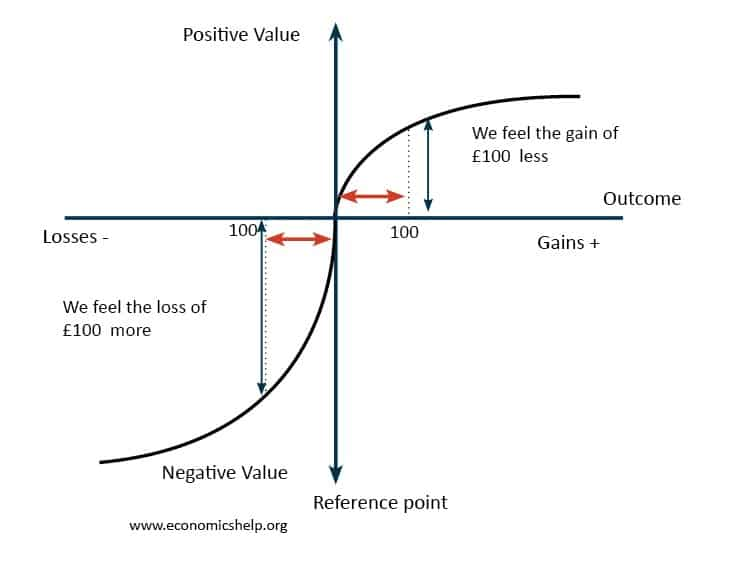
\includegraphics[scale=0.35]{prospect-theory.jpg}
\end{center}
\end{frame}

%@@@@@@@@@@@@@@@@@@@@@@@@@@@@@@@@@@@@@@@@@@@@@@@@@
\begin{frame}
\frametitle{How are incentives supposed work?}
\begin{center}
\Large Incentives are designed by one group (e.g. policy analysts), applied by another (e.g. exec branch bureaucrats), and received by a third (e.g. individuals, firms, etc.).
\end{center}
\end{frame}

%@@@@@@@@@@@@@@@@@@@@@@@@@@@@@@@@@@@@@@@@@@@@@@@@@
\begin{frame}
\frametitle{How are incentives supposed work?}

\begin{itemize}
\item Four parts: Designer, Giver; Target; Incentive;
\bigskip
\bigskip
\item Incentive-based policies are implicitly \textbf{based on utilitarian behavioral model}:
\begin{itemize}
\item Targets are rational w/ well-defined preferences and take purposive action in pursuit;
%\item Which action is taken without incentive?  Which action will be taken with incentives?  (Assume utility maximization);
\item Targets can choose, are prospective, and are unitary (why must they be unitary?);
\end{itemize}
\bigskip
\bigskip
\item In the polis Giver/Target may be collective entities with some inner conflict and some ability to act as a unified group;
\begin{itemize}
\item Giver: city common council, large executive branch agency (e.g. IRS, State Dept);
\item Target: a single person heading a firm, organization, or government entity (what about Arrow's Theorem?).
\end{itemize}
\end{itemize}

\end{frame}

%@@@@@@@@@@@@@@@@@@@@@@@@@@@@@@@@@@@@@@@@@@@@@@@@@
\begin{frame}
\frametitle{Designing Incentives}

\begin{itemize}
\item Effective incentive design requires a good causal model;
\begin{itemize}
\item Numerous penalties and rewards structure any actor's life PRIOR to another intervention;
\item If problem is rooted in institutional/historical patterns targeting a small group is likely ineffective;
%\item Example: cash for school attendance... what about home/family structure, language/cultural barriers, poverty?
\end{itemize}
\bigskip
\item Requires understanding the social relations incentives create:
\begin{itemize}
\item What is the baseline?
\item Positive incentives can create bonds of obligation through reciprocity -- an alliance;
\item Negative incentives can create an adversarial relationship;
\item Successful negative incentives are free, successful positive incentives are costly;
\item Both imply unequal power: one party sets terms/rules, monitors behavior, and decides whether to dispense consequences;
\end{itemize}
\bigskip
\item Example: time horizons.
\end{itemize}

\end{frame}

%@@@@@@@@@@@@@@@@@@@@@@@@@@@@@@@@@@@@@@@@@@@@@@@@@
\begin{frame}
\frametitle{Implementation in the polis}

\begin{itemize}
\item Gaps between Designers and Givers --  people don't usually want to cause suffering by meting out penalties:
\begin{itemize}
\item professional disciplinary board reluctant to revoke licenses;
\item Best undergraduate thesis recommendations;
\item Mandatory minimums, Medieval juries;
\item Poor incentive design $=$ penalties that can't be used;
\end{itemize}
\bigskip
\bigskip
\item Gaps between Designers and Targets:
\begin{itemize}
\item Differences in understanding of meaning (e.g. high school);
\item Targets are strategic and adaptive (e.g. firms pass penalties on to consumers);
\item Pay for performance schemes;
\item Worker safety at DuPont.
\end{itemize}
\end{itemize}

\end{frame}

%@@@@@@@@@@@@@@@@@@@@@@@@@@@@@@@@@@@@@@@@@@@@@@@@@
\begin{frame}
\frametitle{Some things to be aware of...}

\begin{itemize}
\item Make no mistake: incentives are an exercise of power;
\bigskip
\bigskip
\bigskip
\item Incentives can be demeaning;
\bigskip
\bigskip
\bigskip
\item Incentives can undermine public spirit.
\end{itemize}

\end{frame}

%@@@@@@@@@@@@@@@@@@@@@@@@@@@@@@@@@@@@@@@@@@@@@@@@@
\begin{frame}

\begin{center}
\Huge\textbf{Why should we care?}\\
\bigskip
\bigskip
\large Incentives are the currency of policymaking -- many of the recommendations you've made are probably expressible as incentives.  These are factors that increase/diminish the likelihood the incentive structure you assemble will succeed.
\\
\end{center}

\end{frame}

%@@@@@@@@@@@@@@@@@@@@@@@@@@@@@@@@@@@@@@@@@@@@@@@@@
\begin{frame}

\begin{center}
\Huge\textbf{Problems : Rules}\\
\bigskip
\bigskip
\large The essential form of social coordination
\end{center}

\end{frame}

%@@@@@@@@@@@@@@@@@@@@@@@@@@@@@@@@@@@@@@@@@@@@@@@@@
\begin{frame}
\frametitle{What is a rule?}
\begin{center}
\Large A statement that prescribes \textbf{actions} to be taken in certain \textbf{contexts}.
\end{center}
\end{frame}

%@@@@@@@@@@@@@@@@@@@@@@@@@@@@@@@@@@@@@@@@@@@@@@@@@
\begin{frame}
\frametitle{What is a rule?}

\begin{itemize}
\item Rules have two parts: \textbf{actions} and \textbf{contexts}:
\begin{itemize}
\item Actions are usually well-defined and consistent with the Constitution;
\item Context $=$ personal identity, credentialing, location, time, combinations thereof;
\item Ambiguity of contexts create fuzzy boundaries;
\end{itemize}
\bigskip
\bigskip
\item Example: If LWRF discharges to a non-point source that is the functional equivalent of a direct discharge then it must apply for an NPDES permit;
\bigskip
\bigskip
\item Example: If LWRF applies for and receives an NPDES permit then it can dispense treated wastewater into class V wells.
\end{itemize}
\end{frame}

%@@@@@@@@@@@@@@@@@@@@@@@@@@@@@@@@@@@@@@@@@@@@@@@@@
\begin{frame}
\footnotesize 40 CFR 230.3(s)  The term waters of the United States means:
\begin{enumerate}
\item All waters which are currently used, or were used in the past, or may be susceptible to use in interstate or foreign commerce, including all waters which are subject to the ebb and flow of the tide;
\item All interstate waters including interstate wetlands;
\item All other waters such as intrastate lakes, rivers, streams (including intermittent streams), mudflats, sandflats, wetlands, sloughs, prairie potholes, wet meadows, playa lakes, or natural ponds, the use, degradation or destruction of which could affect interstate or foreign commerce including any such waters: 
\begin{enumerate}
\item Which are or could be used by interstate or foreign travelers for recreational or other purposes;
\item From which fish or shellfish are or could be taken and sold in interstate or foreign commerce;
\item Which are used or could be used for industrial purposes by industries in interstate commerce;
\end{enumerate}
\item All impoundments of waters otherwise defined as waters of the United States under this definition;
\item Tributaries of waters identified in paragraphs (s)(1) through (4) of this section;
\item The territorial sea;
\item Wetlands adjacent to waters (other than waters that are themselves wetlands) identified in paragraphs (s)(1) through (6) of this section; waste treatment systems, including treatment ponds or lagoons designed to meet the requirements of CWA (other than cooling ponds as defined in 40 CFR 423.11(m) which also meet the criteria of this definition) are not waters of the United States.
\end{enumerate}
\end{frame}

%@@@@@@@@@@@@@@@@@@@@@@@@@@@@@@@@@@@@@@@@@@@@@@@@@
\begin{frame}
\frametitle{What do rules do and how do they work?}

\begin{itemize}
\item A rule may:
\begin{itemize}
\item Mandate behavior (e.g. contracts, wills, lawsuits);
\item Confer power (e.g. rules that agencies and local governments must follow to make policy);
\end{itemize}
\bigskip
\item Rules require judgements of the form: these things are \textbf{like} the context of the rule so the action applies;
\begin{itemize}
\item To judge things as like or different requires selecting some features and ignoring others;
\item e.g. people by age or location;
\end{itemize}
\bigskip
\item Why do we follow rules?
\begin{itemize}
\item Sanctions befall us if we do not;
\item Rules are \textbf{legitimate} -- perceived as good and right by those who behavior they are meant to control.
\end{itemize}

\end{itemize}

\end{frame}

%@@@@@@@@@@@@@@@@@@@@@@@@@@@@@@@@@@@@@@@@@@@@@@@@@
\begin{frame}
\frametitle{Choices: role of discretion}

\begin{itemize}
\item A good rule should be precise enough to accomplish its purpose and prevent people from manipulating it in ways that undermine its intent (no discretion):
\begin{itemize}
\item Like cases treated alike;
\item Insulate citizens from the whims, prejudices, or personal predilections of officials;
\item Predictability;
\item Drawbacks: insensitive to individual/contextual differences, stifle creative responses to new situations, are easily outdated;
\end{itemize}
\bigskip
\item A good rule should be flexible enough to be useful (yes discretion):
\begin{itemize}
\item Allow sensitivity to individual/contextual differences;
\item Empowers creative responses to new situations;
\item Allows for tacit knowledge (e.g. ``I can’t define it, but I know it when I see it" -- Justice Potter Stewart);
\item Symbolizes ideals and aspirations (e.g. the evolution of the 14th amendment);
\end{itemize}
%\bigskip
%\item ``The proper goal is to eliminate unnecessary discretionary power, not eliminate discretionary power." -- Kenneth Culp Davis, Discretionary Justice.
\end{itemize}

\end{frame}

%%@@@@@@@@@@@@@@@@@@@@@@@@@@@@@@@@@@@@@@@@@@@@@@@@@
%\begin{frame}
%\frametitle{Making Rules}
%
%\begin{itemize}
%\item Focusing events inspire big promises:
%\begin{itemize}
%\item American Revolution $\Rightarrow$ US Constitution;
%\item Great Depression $\Rightarrow$ Social Security Act, New Deal;
%\item Silent Spring $\Rightarrow$ DDT ban, EPA;
%\item Cuyahoga River fire $\Rightarrow$ Clean Water Act;
%\item 9/11 $\Rightarrow$ Patriot act, Dept. of Homeland Security;
%\item Great Recession $\Rightarrow$ Dodd--Frank;
%\item COVID $\Rightarrow$ ???
%\end{itemize}
%\bigskip
%\bigskip
%\item Legislators often avoid specifics that might anger any constituent group:
%\begin{itemize}
%\item Constituency service;
%\item Logrolling;
%\item Symbolic legislation;
%\item Delegation of broad or ambiguous rulemaking authority.
%\end{itemize}
%\bigskip
%\bigskip
%\item Does the US electoral system create a drive towards ambiguity?
%\end{itemize}
%
%\end{frame}

%@@@@@@@@@@@@@@@@@@@@@@@@@@@@@@@@@@@@@@@@@@@@@@@@@
\begin{frame}
\frametitle{Choices: enforcement}

\begin{itemize}
\item Enforcement requires monitoring:
\begin{itemize}
\item Police patrol model $=$ enforcers look for violations;
\item Fire alarm model $=$ enforcers rely on individuals to report violations;
\item Under certain circumstances fire alarm model is more efficient;
\item May depend on details of information environment;
\end{itemize}
\bigskip
\bigskip
%\item Rules allocate privilege and power... fuzziness at the boundaries create incentives for people to portray
%themselves as falling ``on the right side of the law."
%\bigskip
%\bigskip
%\item Rules of thumb -- informal guidelines about violations that seek to fit the punishment
%to the crime in a way that matches a sense of justice (derived from social customs, peer norms, moral beliefs, and
%existing practices);
%\bigskip
%\bigskip
\item Rules foster democracy and democracy fosters rules.
\end{itemize}

\end{frame}

%@@@@@@@@@@@@@@@@@@@@@@@@@@@@@@@@@@@@@@@@@@@@@@@@@
\begin{frame}

\begin{center}
\Huge\textbf{Why should we care?}\\
\bigskip
\bigskip
\large Rule generate practical metaphors -- they create consequences for likeness and are how incentives are operationalized.
\\
\end{center}

\end{frame}

%@@@@@@@@@@@@@@@@@@@@@@@@@@@@@@@@@@@@@@@@@@@@@@@@@
\begin{frame}

\begin{center}
\Huge\textbf{Problems : Facts}\\
\bigskip
\bigskip
\large The currency of persuasion
\end{center}

\end{frame}

%@@@@@@@@@@@@@@@@@@@@@@@@@@@@@@@@@@@@@@@@@@@@@@@@@
\begin{frame}
\frametitle{An experiment: which do you think is right?}

\begin{itemize}
\item ``Civil government, so far as it is instituted for the security of property, is in reality instituted for the defense of the rich against the poor, or of those who have some property against those who have none at all."  (Karl Marx, \textit{The Communist Manifesto})
\bigskip
\bigskip
\item ``Society does not consist of individuals but expresses the sum of interrelations, the relations within which these individuals stand." (John Stuart Mill, \textit{On Liberty})
\bigskip
\bigskip
\item ``The laws of property have made property of things which never ought to be property, and absolute property where only a qualified property ought to exist. They have not held the balance fairly between human beings, but have heaped impediments upon some, to give advantage to others; they have purposely fostered inequalities, and prevented all from starting fair in the race." (Friedrich Engels, \textit{The Communist Manifesto})
\end{itemize}

\end{frame}

%@@@@@@@@@@@@@@@@@@@@@@@@@@@@@@@@@@@@@@@@@@@@@@@@@
\begin{frame}
\frametitle{An experiment: which do you think is right?  Turns out I lied... did the speaker matter?}

\begin{itemize}
\item ``Civil government, so far as it is instituted for the security of property, is in reality instituted for the defense of the rich against the poor, or of those who have some property against those who have none at all."  (Adam Smith)
\bigskip
\bigskip
\item ``Society does not consist of individuals but expresses the sum of interrelations, the relations within which these individuals stand." (Karl Marx)
\bigskip
\bigskip
\item ``The laws of property have made property of things which never ought to be property, and absolute property where only a qualified property ought to exist. They have not held the balance fairly between human beings, but have heaped impediments upon some, to give advantage to others; they have purposely fostered inequalities, and prevented all from starting fair in the race." (John Stuart Mill)
\end{itemize}

\end{frame}

%@@@@@@@@@@@@@@@@@@@@@@@@@@@@@@@@@@@@@@@@@@@@@@@@@
\begin{frame}
\frametitle{Making Facts in the Polis}

\begin{columns}
\begin{column}{0.5\textwidth}
\begin{itemize}
\item There is no such thing as a fact!  Facts don't exist independent of interpretive lenses:
\begin{itemize}
\item Words (e.g. classification as gaming or gambling);
\item Statistical choices in science (e.g. how to count, model specification);
\item POV (e.g. unreliable witnesses -- indeed facts themselves are under dispute in a trial);
\end{itemize}
\bigskip
\item The doubt strategy: Industry science-based challenges to research $\Rightarrow$ ``flaws mean that finding is no more than an unproven hypothesis" (e.g. tobacco industry);
\end{itemize}
\end{column}
\begin{column}{0.5\textwidth}
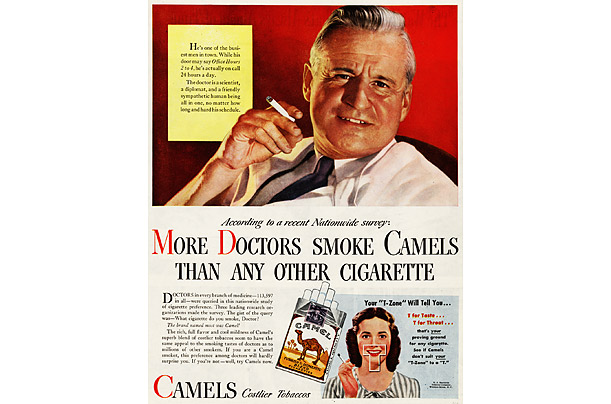
\includegraphics[scale=0.4]{smoking.jpg}
\end{column}
\end{columns}

\end{frame}

%@@@@@@@@@@@@@@@@@@@@@@@@@@@@@@@@@@@@@@@@@@@@@@@@@
\begin{frame}
\frametitle{Making Facts in the Polis}

\begin{columns}
\begin{column}{0.5\textwidth}
\begin{itemize}
\item There is no such thing as a fact!  Facts don't exist independent of interpretive lenses:
\begin{itemize}
\item Words (e.g. classification as gaming or gambling);
\item Statistical choices in science (e.g. how to count, model specification);
\item POV (e.g. unreliable witnesses -- indeed facts themselves are under dispute in a trial);
\end{itemize}
\bigskip
\item The doubt strategy: Industry science-based challenges to research $\Rightarrow$ ``flaws mean that finding is no more than an unproven hypothesis" (e.g. tobacco industry);
\end{itemize}
\end{column}
\begin{column}{0.5\textwidth}
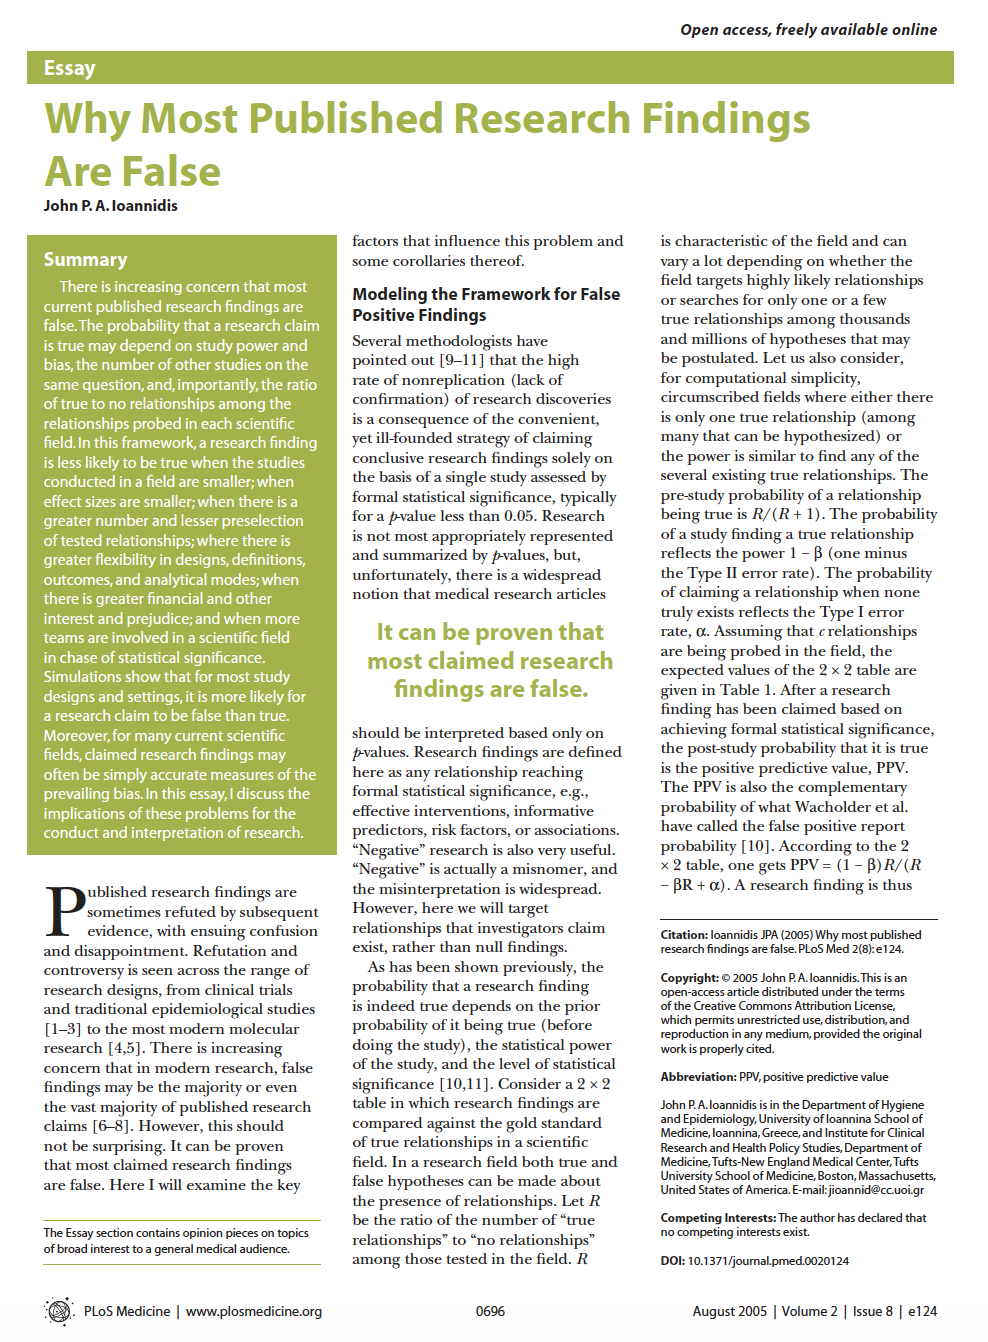
\includegraphics[scale=0.3]{False_pubs.png}
\end{column}
\end{columns}

\end{frame}

%@@@@@@@@@@@@@@@@@@@@@@@@@@@@@@@@@@@@@@@@@@@@@@@@@
\begin{frame}
\frametitle{Two faces of persuasion}

\begin{itemize}
%\item ``To be political, to be in a polis, meant that everything was decided through words and persuasion and not through force and violence" -- Hannah Arendt
%\bigskip
%\bigskip
%\bigskip
\item \textbf{Persuasion can be enlightenment}: science, evidence, logic, reason, rationality obviate the need for violence... NOT emotion, biases, loyalty, or passion;
\bigskip
\bigskip
\bigskip
\item \textbf{Persuasion can be propaganda or indoctrination}: manipulation via appeals to fear and anxiety $\Rightarrow$ stymies capacity for independent thought.
\end{itemize}

\end{frame}

%@@@@@@@@@@@@@@@@@@@@@@@@@@@@@@@@@@@@@@@@@@@@@@@@@
\begin{frame}
\frametitle{Challenges to becoming informed}

\begin{itemize}
\item How do we distinguish \textbf{information} and \textbf{education} from \textbf{propaganda} and \textbf{indoctrination}?
\bigskip
\bigskip
\item Factors that divert us from rational consideration of information:
\begin{itemize}
\item source (race/looks/manners/reputation);
\item emotion;
\item composition of group;
%\item ignorance;
\end{itemize}
%\bigskip
%\bigskip
%\item Example -- Bush tax cuts:
%\begin{itemize}
%\item Majority of citizens believe the rich pay too little in taxes and the poor pay too much;
%\item Citizens who thought their own tax burden was too high favored the cuts;
%\item Those who think govt "wastes a lot of money" were less supportive of the cuts;
%\end{itemize}
\bigskip
\bigskip
\item Example -- Are statements doubting human-caused climate change propaganda?  Always?  Sometimes?  Never?
\end{itemize}

\end{frame}

%@@@@@@@@@@@@@@@@@@@@@@@@@@@@@@@@@@@@@@@@@@@@@@@@@
\begin{frame}
\frametitle{Indoctrination}

\begin{itemize}
\item Definition:
\begin{itemize}
\item A regime in which dominant elites shape people's beliefs and knowledge...
\item ...in a manipulative and self-interested way...
\item ...that deprives them of the capacity for independent thinking;
\end{itemize}
\bigskip
\bigskip
\item The power of business to persuade:
\begin{itemize}
\item pivotal position in capitalist economies;
\item overwhelming financial and organizational resources to shape political culture and influence elections;
\item manipulation of scientific information to serve its economic interests;
\item control of the media;
\end{itemize}
\bigskip
\bigskip
\item The power of government to persaude:
\begin{itemize}
\item Supplying information (e.g. Iraq war former military officer commentators);
\item Withholding information (e.g. casualty counts);
\item Low level bureaucrat action (e.g. voter registration in the south).
\end{itemize}
\bigskip
\bigskip
\item blar
\end{itemize}

\end{frame}

%@@@@@@@@@@@@@@@@@@@@@@@@@@@@@@@@@@@@@@@@@@@@@@@@@
\begin{frame}

\begin{center}
\Huge\textbf{Why should we care?}\\
\bigskip
\bigskip
\large We have treated peer reviewed publications as facts -- they are not.
\\
\end{center}

\end{frame}

%@@@@@@@@@@@@@@@@@@@@@@@@@@@@@@@@@@@@@@@@@@@@@@@@@
\begin{frame}

\begin{center}
\Huge\textbf{Problems : Rights}\\
\bigskip
\bigskip
\large Formalized political demands
\end{center}

\end{frame}

%@@@@@@@@@@@@@@@@@@@@@@@@@@@@@@@@@@@@@@@@@@@@@@@@@
\begin{frame}
\frametitle{Traditions of Rights}

\begin{itemize}
\item \textbf{Realist}: rights are citizens' claims backed by the power of the state;
\begin{itemize}
\item Expectations realized by invoking government;
\item Rights do not exist outside the laws of particular political systems;
\end{itemize}
\bigskip
\bigskip
\item \textbf{Normative}: rights are moral principles;
\begin{itemize}
\item Found in natural law, religious texts, rational thought, public opinion, social practices and institutions, and the idea of universal human rights;
\item Derived from some source other than the power of enforcement;
\item Rights can exist without being actively claimed or backed by the state;
\end{itemize}
\bigskip
\bigskip
\item These two forms of rights are unified in the polis:
\begin{itemize}
\item Aggrieved groups organize to claim new rights not yet legally recognized (normative);
\item They also act to ensure that rights formalized in law are applied (realist);
\end{itemize}
\bigskip
\bigskip
\item Were the founders realists or normativists in terms of rights?
\end{itemize}

\end{frame}

%@@@@@@@@@@@@@@@@@@@@@@@@@@@@@@@@@@@@@@@@@@@@@@@@@
\begin{frame}
\frametitle{Rights as policies}

\begin{itemize}
\item Typology:
\begin{itemize}
\item Procedural -- decision must be made in a certain way, outcome not guaranteed (e.g. trial by jury of peers);
\item Negative substantive -- specific entitlements of non-interference (no second party required) 
\item Positive substantive -- specific entitlements expressed duties required of a second party;
\item All define relationships;
\end{itemize}
\bigskip
\bigskip
\item Step 1) Official statement of the right:
\begin{itemize}
\item Statutory/Administrative law/Precedential (Common) law;
\end{itemize}
\bigskip
\bigskip
\item Step 2) Grievance process:
\begin{itemize}
\item two parties—one claiming a right denied, the other alleged to have denied the right—air their dispute via reasoned argument
before a neutral third party;
\item Decision comes through application of preexisting rules to the facts of the particular dispute;
\end{itemize}
\bigskip
\bigskip
\item Step 3) Enforcement -- threat of force.
\end{itemize}

\end{frame}

%@@@@@@@@@@@@@@@@@@@@@@@@@@@@@@@@@@@@@@@@@@@@@@@@@
\begin{frame}
\frametitle{Creating rights in the polis}

\begin{itemize}
\item \textbf{Normative} -- disjunction between perceptions of moral rights and lived experiences in political practice drives rights-claiming (e.g. Brown v Board of Education);
\bigskip
\bigskip
\item \textbf{Sociological} -- sociological arguments often used to characterize change to justify a break from precedent -- these are always interpreted through political and ideological lenses (e.g. the lifespan of the Voting Rights Act);
\bigskip
\bigskip
\item \textbf{Political}:
\begin{itemize}
\item Ideal: identity should not change access to courts or probability of victory therein;
\item Polis: differing social positions that give the more or less power w.r.t courts;
\item Repeat players -- low value for any one case, interested in general declaration of rights that will manage future cases;
\item One shot players -- high value on tangible outcome of current case;
\item Power and resources disparities between repeat players and one shotters implies they are not equal before the law;
\item Strategic manipulation via test cases -- seeking plantiffs with a high probability of winning;
\end{itemize}
\end{itemize}

\end{frame}

%@@@@@@@@@@@@@@@@@@@@@@@@@@@@@@@@@@@@@@@@@@@@@@@@@
\begin{frame}

\begin{center}
\Huge\textbf{Why should we care?}\\
\bigskip
\bigskip
\large Rights work by dramatizing power relationships as personal stories, by legitimizing political demands, by mobilizing new political alliances, and, eventually, by transforming social institutions.
\\
\end{center}

\end{frame}

%@@@@@@@@@@@@@@@@@@@@@@@@@@@@@@@@@@@@@@@@@@@@@@@@@
\begin{frame}

\begin{center}
\Huge\textbf{Problems : Powers}\\
\bigskip
\bigskip
\large The structure of decision-making institutions
\end{center}

\end{frame}

%@@@@@@@@@@@@@@@@@@@@@@@@@@@@@@@@@@@@@@@@@@@@@@@@@
\begin{frame}
\frametitle{What is power?}

\begin{itemize}
\item \textbf{Power} $=$ \textbf{authority} and \textbf{capacity} to act;
\begin{itemize}
\item Authority $=$ making policy decisions;
\item Capacity $=$ carrying out policy decisions;
\item For us, this is determined by the constitution;
\end{itemize}
\bigskip
\bigskip
\item In the polis, policies that reform decision-making processes are the most consequential political strategy;
\begin{itemize}
\item Process changes $=$ changing who makes the decision $=$ reallocations of power;
\item Attempts by someone who is not winning in one arena to shift decision making to a different arena where they might prevail;
\item The framers understood the consequentialism which is why constitutional amendments are hard to do;
\end{itemize}
\bigskip
\bigskip
\item Two perspectives on process changes:
\begin{itemize}
\item Does this change solve the nominal problem?
\item Who gains the right to participate in decisions about the problem?
\end{itemize}
\end{itemize}

\end{frame}

%@@@@@@@@@@@@@@@@@@@@@@@@@@@@@@@@@@@@@@@@@@@@@@@@@
\begin{frame}
\frametitle{Variations of institutional reform}

\begin{itemize}
\item Membership -- voting and citizenship:
\begin{itemize}
\item Paradox: government controlled by the people, yet can choose their citizens;
\item Balance benefits for membership with costs to democracy for exclusion;
\end{itemize}
\item Representation -- selecting leaders:
\begin{itemize}
\item Substantive representation $=$ shared goals;
\item Descriptive representation $=$ shared characteristics (e.g. Voting Rights Act);
\item Delegation;
\end{itemize}
\item Centralizing and decentralizing power:
\begin{itemize}
\item Federalism: combine autonomy of members with uniform policymaking by central authority;
\item Organization of authority is always a struggle over power -- who benefits (e.g. income redistribution);
\end{itemize}
\item Accountability:
\begin{itemize}
\item Paradox: people choose leaders who subsequently control people -- accountability is intended to resolve this;
\end{itemize}
\item Privatization:
\begin{itemize}
\item ``outsourcing sovereignty" (e.g. prison management, deregulation, govt procurement);
\end{itemize}
\end{itemize}

\end{frame}

%@@@@@@@@@@@@@@@@@@@@@@@@@@@@@@@@@@@@@@@@@@@@@@@@@
\begin{frame}
\begin{table}[]
\begin{tabular}{cccc}
 & \textbf{Articles of Confederation (1776)} & \textbf{Constitution (1789)} & \\
 &unicameralism&bicameralism& \\
  &1 state 1 vote&1 rep 1 vote&\\
&power distributed across states&Federalism (superior/subordinates)&\\
&No universal citizen rights&Citizens $=$ in all states, rights formalized (BoR)&\\
&Support from 9/13 states required &Passage by Congress/President&\\
&to enforce law everywhere&to enforce law everywhere&
\end{tabular}
\end{table}
\end{frame}

%@@@@@@@@@@@@@@@@@@@@@@@@@@@@@@@@@@@@@@@@@@@@@@@@@
\begin{frame}

\begin{center}
\Huge\textbf{Why should we care?}\\
\bigskip
\bigskip
\large The audience for your policy can only take actions circumscribed by the powers delegated to them... though they may be able to propose changes in institutional makeup.\\
\end{center}

\end{frame}

%@@@@@@@@@@@@@@@@@@@@@@@@@@@@@@@@@@@@@@@@@@@@@@@@@
\begin{frame}
\frametitle{Birkland$+$ Model of Policy, goals, problems}
\begin{itemize}
\item Policy Domain: what substantive problems are under consideration?  This specifies:
\begin{itemize}
\item The actors involved, official actors who can make decisions $+$ \textbf{stakeholders}; 
\item \textbf{Distribution of benefits/costs} $\Rightarrow$ actor organization, e.g. iron triangle, policy community;
\item The systemic agenda; 
\end{itemize}
\bigskip
\item \color{black}Input-output Model;
\begin{itemize}
\item Actors: legislature, executive, bureaucrats, justices and the available levers;
\item Inputs: \textbf{agenda setting (application of power/social construction, focusing events, indicator change driven esp by unofficial actors)} \textbf{sets goals}, \textbf{determines the causal model}, which specifies the institutional agenda, and leads to the policies on the decision agenda;
\item Black box \textbf{decision making, timing (incrementalism, punctuated eq) driven by indicators/focusing events}, choice driven by e.g. median voter thm, Arrow's thm;
\begin{itemize}
\item Round 1: works on decision agenda, leads to outputs (e.g. statute laws, rules, court decisions);
\item Round 2: Implementation, leads to outcomes;
 \end{itemize}
\end{itemize}
\bigskip
\item Outcomes: \textbf{Feedback from failure and success}, learning leads to iteration and updates.
\end{itemize}
\end{frame}

%@@@@@@@@@@@@@@@@@@@@@@@@@@@@@@@@@@@@@@@@@@@@@@@@@
\begin{frame}
\frametitle{Birkland$+$ Model of Policy, goals, problems}
\begin{itemize}
\item Policy Domain: what substantive problems are under consideration?  This specifies:
\begin{itemize}
\item The actors involved, official actors who can make decisions $+$ \textbf{stakeholders}; 
\item \textbf{Distribution of benefits/costs} $\Rightarrow$ actor organization, e.g. iron triangle, policy community;
\item The systemic agenda; 
\end{itemize}
\bigskip
\item \color{black}Input-output Model;
\begin{itemize}
\item Actors: \textbf{legislature, executive, bureaucrats, justices and the available levers};
\item Inputs: \textbf{agenda setting (application of power/social construction, focusing events, indicator change driven esp by unofficial actors)} \textbf{sets goals}, \textbf{determines the causal model}, which specifies the institutional agenda, and leads to the \textbf{policies} on the decision agenda;
\item Black box \textbf{decision making, timing (incrementalism, punctuated eq) driven by indicators/focusing events}, choice driven by e.g. median voter thm, Arrow's thm;
\begin{itemize}
\item Round 1: \textbf{works on decision agenda}, leads to outputs (e.g. statute laws, rules, court decisions);
\item Round 2: \textbf{Implementation}, leads to outcomes;
 \end{itemize}
\end{itemize}
\bigskip
\item Outcomes: \textbf{Feedback from failure and success}, learning leads to iteration and updates.
\end{itemize}
\end{frame}

\end{document}






